% Created by tikzDevice version 0.8.1 on 2015-12-07 17:04:29
% !TEX encoding = UTF-8 Unicode
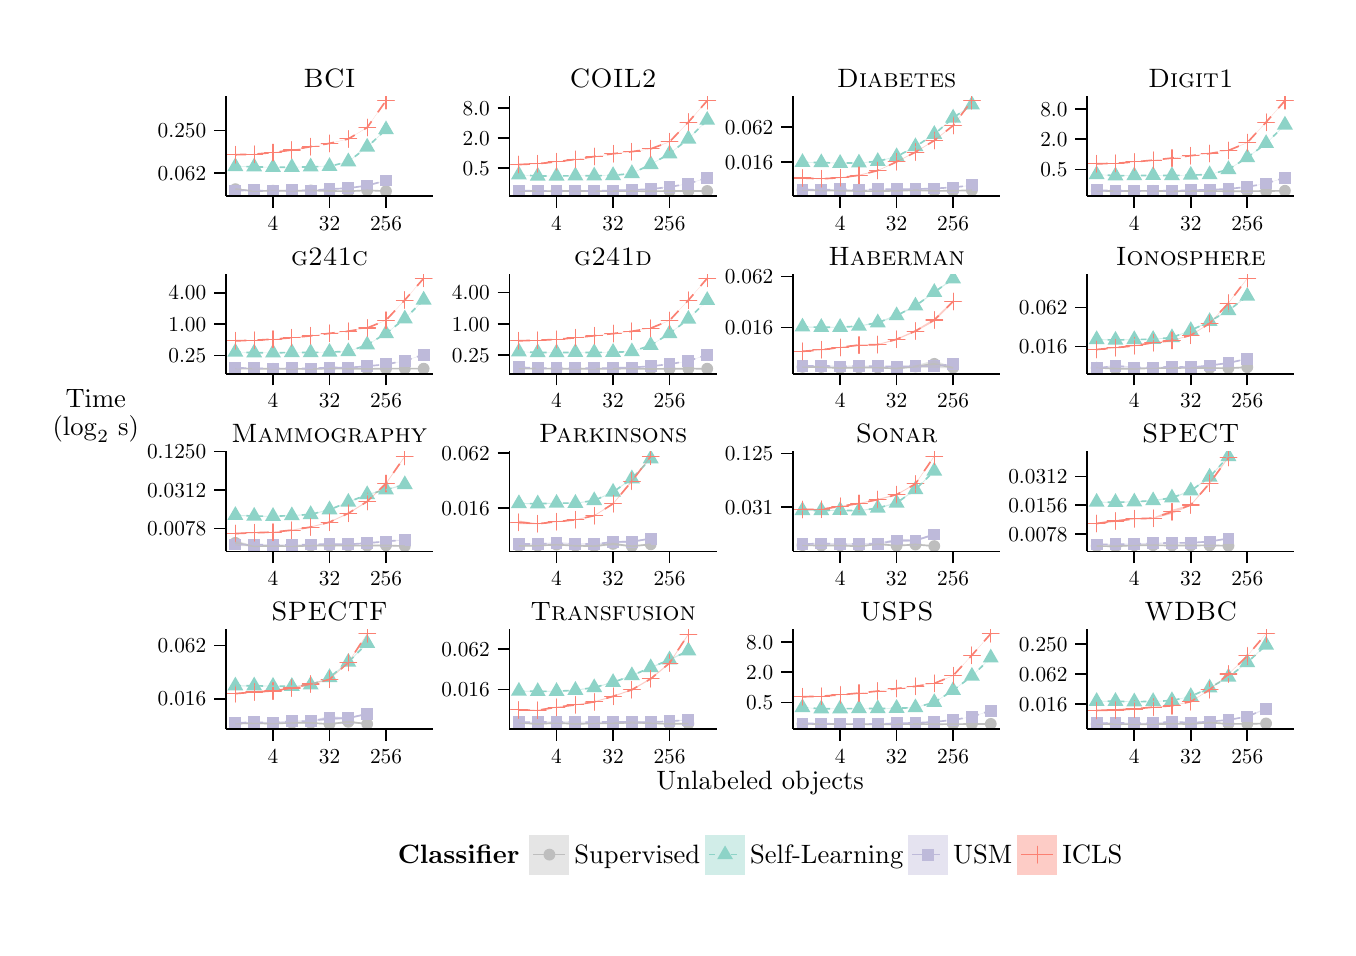
\begin{tikzpicture}[x=1pt,y=1pt]
\definecolor{fillColor}{RGB}{255,255,255}
\path[use as bounding box,fill=fillColor,fill opacity=0.00] (0,0) rectangle (469.75,325.21);
\begin{scope}
\path[clip] (  0.00,  0.00) rectangle (469.75,325.21);
\definecolor{drawColor}{RGB}{255,255,255}
\definecolor{fillColor}{RGB}{255,255,255}

\path[draw=drawColor,line width= 0.6pt,line join=round,line cap=round,fill=fillColor] (  0.00,  0.00) rectangle (469.76,325.21);
\end{scope}
\begin{scope}
\path[clip] ( 71.64,264.38) rectangle (146.49,300.54);
\definecolor{fillColor}{RGB}{255,255,255}

\path[fill=fillColor] ( 71.64,264.38) rectangle (146.49,300.54);
\definecolor{fillColor}{RGB}{190,190,190}

\path[fill=fillColor] ( 75.05,266.86) circle (  2.13);
\definecolor{fillColor}{RGB}{141,211,199}

\path[fill=fillColor] ( 75.05,278.37) --
	( 77.92,273.39) --
	( 72.17,273.39) --
	cycle;
\definecolor{fillColor}{RGB}{190,186,218}

\path[fill=fillColor] ( 72.91,264.22) --
	( 77.18,264.22) --
	( 77.18,268.49) --
	( 72.91,268.49) --
	cycle;
\definecolor{drawColor}{RGB}{251,128,114}

\path[draw=drawColor,line width= 0.4pt,line join=round,line cap=round] ( 72.03,279.30) -- ( 78.06,279.30);

\path[draw=drawColor,line width= 0.4pt,line join=round,line cap=round] ( 75.05,276.28) -- ( 75.05,282.32);
\definecolor{fillColor}{RGB}{190,190,190}

\path[fill=fillColor] ( 81.85,266.14) circle (  2.13);
\definecolor{fillColor}{RGB}{141,211,199}

\path[fill=fillColor] ( 81.85,278.28) --
	( 84.72,273.30) --
	( 78.98,273.30) --
	cycle;
\definecolor{fillColor}{RGB}{190,186,218}

\path[fill=fillColor] ( 79.72,264.31) --
	( 83.98,264.31) --
	( 83.98,268.58) --
	( 79.72,268.58) --
	cycle;

\path[draw=drawColor,line width= 0.4pt,line join=round,line cap=round] ( 78.83,279.49) -- ( 84.87,279.49);

\path[draw=drawColor,line width= 0.4pt,line join=round,line cap=round] ( 81.85,276.47) -- ( 81.85,282.51);
\definecolor{fillColor}{RGB}{190,190,190}

\path[fill=fillColor] ( 88.65,266.31) circle (  2.13);
\definecolor{fillColor}{RGB}{141,211,199}

\path[fill=fillColor] ( 88.65,278.06) --
	( 91.53,273.08) --
	( 85.78,273.08) --
	cycle;
\definecolor{fillColor}{RGB}{190,186,218}

\path[fill=fillColor] ( 86.52,263.98) --
	( 90.79,263.98) --
	( 90.79,268.25) --
	( 86.52,268.25) --
	cycle;

\path[draw=drawColor,line width= 0.4pt,line join=round,line cap=round] ( 85.64,280.08) -- ( 91.67,280.08);

\path[draw=drawColor,line width= 0.4pt,line join=round,line cap=round] ( 88.65,277.06) -- ( 88.65,283.10);
\definecolor{fillColor}{RGB}{190,190,190}

\path[fill=fillColor] ( 95.46,266.22) circle (  2.13);
\definecolor{fillColor}{RGB}{141,211,199}

\path[fill=fillColor] ( 95.46,278.11) --
	( 98.33,273.13) --
	( 92.58,273.13) --
	cycle;
\definecolor{fillColor}{RGB}{190,186,218}

\path[fill=fillColor] ( 93.32,264.28) --
	( 97.59,264.28) --
	( 97.59,268.54) --
	( 93.32,268.54) --
	cycle;

\path[draw=drawColor,line width= 0.4pt,line join=round,line cap=round] ( 92.44,281.01) -- ( 98.48,281.01);

\path[draw=drawColor,line width= 0.4pt,line join=round,line cap=round] ( 95.46,277.99) -- ( 95.46,284.02);
\definecolor{fillColor}{RGB}{190,190,190}

\path[fill=fillColor] (102.26,266.38) circle (  2.13);
\definecolor{fillColor}{RGB}{141,211,199}

\path[fill=fillColor] (102.26,278.25) --
	(105.14,273.28) --
	( 99.39,273.28) --
	cycle;
\definecolor{fillColor}{RGB}{190,186,218}

\path[fill=fillColor] (100.13,264.24) --
	(104.40,264.24) --
	(104.40,268.51) --
	(100.13,268.51) --
	cycle;

\path[draw=drawColor,line width= 0.4pt,line join=round,line cap=round] ( 99.24,282.22) -- (105.28,282.22);

\path[draw=drawColor,line width= 0.4pt,line join=round,line cap=round] (102.26,279.20) -- (102.26,285.23);
\definecolor{fillColor}{RGB}{190,190,190}

\path[fill=fillColor] (109.07,266.20) circle (  2.13);
\definecolor{fillColor}{RGB}{141,211,199}

\path[fill=fillColor] (109.07,278.41) --
	(111.94,273.43) --
	(106.19,273.43) --
	cycle;
\definecolor{fillColor}{RGB}{190,186,218}

\path[fill=fillColor] (106.93,264.74) --
	(111.20,264.74) --
	(111.20,269.00) --
	(106.93,269.00) --
	cycle;

\path[draw=drawColor,line width= 0.4pt,line join=round,line cap=round] (106.05,283.39) -- (112.08,283.39);

\path[draw=drawColor,line width= 0.4pt,line join=round,line cap=round] (109.07,280.37) -- (109.07,286.41);
\definecolor{fillColor}{RGB}{190,190,190}

\path[fill=fillColor] (115.87,266.09) circle (  2.13);
\definecolor{fillColor}{RGB}{141,211,199}

\path[fill=fillColor] (115.87,280.11) --
	(118.74,275.13) --
	(113.00,275.13) --
	cycle;
\definecolor{fillColor}{RGB}{190,186,218}

\path[fill=fillColor] (113.74,265.06) --
	(118.00,265.06) --
	(118.00,269.33) --
	(113.74,269.33) --
	cycle;

\path[draw=drawColor,line width= 0.4pt,line join=round,line cap=round] (112.85,285.01) -- (118.89,285.01);

\path[draw=drawColor,line width= 0.4pt,line join=round,line cap=round] (115.87,282.00) -- (115.87,288.03);
\definecolor{fillColor}{RGB}{190,190,190}

\path[fill=fillColor] (122.68,266.44) circle (  2.13);
\definecolor{fillColor}{RGB}{141,211,199}

\path[fill=fillColor] (122.68,285.41) --
	(125.55,280.43) --
	(119.80,280.43) --
	cycle;
\definecolor{fillColor}{RGB}{190,186,218}

\path[fill=fillColor] (120.54,266.02) --
	(124.81,266.02) --
	(124.81,270.29) --
	(120.54,270.29) --
	cycle;

\path[draw=drawColor,line width= 0.4pt,line join=round,line cap=round] (119.66,289.13) -- (125.69,289.13);

\path[draw=drawColor,line width= 0.4pt,line join=round,line cap=round] (122.68,286.11) -- (122.68,292.15);
\definecolor{fillColor}{RGB}{190,190,190}

\path[fill=fillColor] (129.48,266.12) circle (  2.13);
\definecolor{fillColor}{RGB}{141,211,199}

\path[fill=fillColor] (129.48,291.68) --
	(132.35,286.71) --
	(126.61,286.71) --
	cycle;
\definecolor{fillColor}{RGB}{190,186,218}

\path[fill=fillColor] (127.35,267.83) --
	(131.61,267.83) --
	(131.61,272.10) --
	(127.35,272.10) --
	cycle;

\path[draw=drawColor,line width= 0.4pt,line join=round,line cap=round] (126.46,298.84) -- (132.50,298.84);

\path[draw=drawColor,line width= 0.4pt,line join=round,line cap=round] (129.48,295.83) -- (129.48,301.86);
\definecolor{drawColor}{RGB}{190,190,190}

\path[draw=drawColor,line width= 0.6pt,line join=round] ( 75.05,266.86) --
	( 81.85,266.14) --
	( 88.65,266.31) --
	( 95.46,266.22) --
	(102.26,266.38) --
	(109.07,266.20) --
	(115.87,266.09) --
	(122.68,266.44) --
	(129.48,266.12);
\definecolor{drawColor}{RGB}{141,211,199}

\path[draw=drawColor,line width= 0.6pt,dash pattern=on 2pt off 2pt ,line join=round] ( 75.05,275.05) --
	( 81.85,274.96) --
	( 88.65,274.74) --
	( 95.46,274.79) --
	(102.26,274.93) --
	(109.07,275.09) --
	(115.87,276.79) --
	(122.68,282.09) --
	(129.48,288.37);
\definecolor{drawColor}{RGB}{190,186,218}

\path[draw=drawColor,line width= 0.6pt,dash pattern=on 4pt off 2pt ,line join=round] ( 75.05,266.36) --
	( 81.85,266.45) --
	( 88.65,266.12) --
	( 95.46,266.41) --
	(102.26,266.38) --
	(109.07,266.87) --
	(115.87,267.20) --
	(122.68,268.16) --
	(129.48,269.96);
\definecolor{drawColor}{RGB}{251,128,114}

\path[draw=drawColor,line width= 0.6pt,dash pattern=on 4pt off 4pt ,line join=round] ( 75.05,279.30) --
	( 81.85,279.49) --
	( 88.65,280.08) --
	( 95.46,281.01) --
	(102.26,282.22) --
	(109.07,283.39) --
	(115.87,285.01) --
	(122.68,289.13) --
	(129.48,298.84);
\definecolor{fillColor}{RGB}{190,190,190}

\path[fill=fillColor,fill opacity=0.40] ( 75.05,267.14) --
	( 81.85,266.24) --
	( 88.65,266.44) --
	( 95.46,266.33) --
	(102.26,266.53) --
	(109.07,266.30) --
	(115.87,266.16) --
	(122.68,266.58) --
	(129.48,266.17) --
	(129.48,266.06) --
	(122.68,266.29) --
	(115.87,266.03) --
	(109.07,266.10) --
	(102.26,266.23) --
	( 95.46,266.11) --
	( 88.65,266.18) --
	( 81.85,266.04) --
	( 75.05,266.57) --
	cycle;
\definecolor{fillColor}{RGB}{141,211,199}

\path[fill=fillColor,fill opacity=0.40] ( 75.05,275.16) --
	( 81.85,275.06) --
	( 88.65,274.81) --
	( 95.46,274.87) --
	(102.26,275.01) --
	(109.07,275.14) --
	(115.87,276.88) --
	(122.68,282.20) --
	(129.48,288.47) --
	(129.48,288.26) --
	(122.68,281.97) --
	(115.87,276.70) --
	(109.07,275.03) --
	(102.26,274.85) --
	( 95.46,274.72) --
	( 88.65,274.66) --
	( 81.85,274.85) --
	( 75.05,274.94) --
	cycle;
\definecolor{fillColor}{RGB}{190,186,218}

\path[fill=fillColor,fill opacity=0.40] ( 75.05,266.48) --
	( 81.85,266.59) --
	( 88.65,266.18) --
	( 95.46,266.53) --
	(102.26,266.46) --
	(109.07,267.00) --
	(115.87,267.28) --
	(122.68,268.26) --
	(129.48,270.08) --
	(129.48,269.85) --
	(122.68,268.05) --
	(115.87,267.11) --
	(109.07,266.74) --
	(102.26,266.30) --
	( 95.46,266.28) --
	( 88.65,266.05) --
	( 81.85,266.30) --
	( 75.05,266.23) --
	cycle;
\definecolor{fillColor}{RGB}{251,128,114}

\path[fill=fillColor,fill opacity=0.40] ( 75.05,279.39) --
	( 81.85,279.57) --
	( 88.65,280.14) --
	( 95.46,281.06) --
	(102.26,282.27) --
	(109.07,283.43) --
	(115.87,285.06) --
	(122.68,289.19) --
	(129.48,298.89) --
	(129.48,298.79) --
	(122.68,289.08) --
	(115.87,284.97) --
	(109.07,283.34) --
	(102.26,282.16) --
	( 95.46,280.95) --
	( 88.65,280.02) --
	( 81.85,279.41) --
	( 75.05,279.21) --
	cycle;
\end{scope}
\begin{scope}
\path[clip] (174.10,264.38) rectangle (248.95,300.54);
\definecolor{fillColor}{RGB}{255,255,255}

\path[fill=fillColor] (174.10,264.38) rectangle (248.95,300.54);
\definecolor{fillColor}{RGB}{190,190,190}

\path[fill=fillColor] (177.51,266.20) circle (  2.13);
\definecolor{fillColor}{RGB}{141,211,199}

\path[fill=fillColor] (177.51,275.36) --
	(180.38,270.38) --
	(174.63,270.38) --
	cycle;
\definecolor{fillColor}{RGB}{190,186,218}

\path[fill=fillColor] (175.37,264.24) --
	(179.64,264.24) --
	(179.64,268.50) --
	(175.37,268.50) --
	cycle;
\definecolor{drawColor}{RGB}{251,128,114}

\path[draw=drawColor,line width= 0.4pt,line join=round,line cap=round] (174.49,275.75) -- (180.52,275.75);

\path[draw=drawColor,line width= 0.4pt,line join=round,line cap=round] (177.51,272.73) -- (177.51,278.77);
\definecolor{fillColor}{RGB}{190,190,190}

\path[fill=fillColor] (184.31,266.15) circle (  2.13);
\definecolor{fillColor}{RGB}{141,211,199}

\path[fill=fillColor] (184.31,274.92) --
	(187.18,269.94) --
	(181.44,269.94) --
	cycle;
\definecolor{fillColor}{RGB}{190,186,218}

\path[fill=fillColor] (182.18,264.13) --
	(186.44,264.13) --
	(186.44,268.40) --
	(182.18,268.40) --
	cycle;

\path[draw=drawColor,line width= 0.4pt,line join=round,line cap=round] (181.29,276.05) -- (187.33,276.05);

\path[draw=drawColor,line width= 0.4pt,line join=round,line cap=round] (184.31,273.03) -- (184.31,279.06);
\definecolor{fillColor}{RGB}{190,190,190}

\path[fill=fillColor] (191.11,266.15) circle (  2.13);
\definecolor{fillColor}{RGB}{141,211,199}

\path[fill=fillColor] (191.11,274.94) --
	(193.99,269.96) --
	(188.24,269.96) --
	cycle;
\definecolor{fillColor}{RGB}{190,186,218}

\path[fill=fillColor] (188.98,264.03) --
	(193.25,264.03) --
	(193.25,268.30) --
	(188.98,268.30) --
	cycle;

\path[draw=drawColor,line width= 0.4pt,line join=round,line cap=round] (188.10,276.75) -- (194.13,276.75);

\path[draw=drawColor,line width= 0.4pt,line join=round,line cap=round] (191.11,273.73) -- (191.11,279.77);
\definecolor{fillColor}{RGB}{190,190,190}

\path[fill=fillColor] (197.92,266.22) circle (  2.13);
\definecolor{fillColor}{RGB}{141,211,199}

\path[fill=fillColor] (197.92,275.01) --
	(200.79,270.03) --
	(195.04,270.03) --
	cycle;
\definecolor{fillColor}{RGB}{190,186,218}

\path[fill=fillColor] (195.78,264.10) --
	(200.05,264.10) --
	(200.05,268.36) --
	(195.78,268.36) --
	cycle;

\path[draw=drawColor,line width= 0.4pt,line join=round,line cap=round] (194.90,277.61) -- (200.94,277.61);

\path[draw=drawColor,line width= 0.4pt,line join=round,line cap=round] (197.92,274.60) -- (197.92,280.63);
\definecolor{fillColor}{RGB}{190,190,190}

\path[fill=fillColor] (204.72,266.12) circle (  2.13);
\definecolor{fillColor}{RGB}{141,211,199}

\path[fill=fillColor] (204.72,275.00) --
	(207.60,270.02) --
	(201.85,270.02) --
	cycle;
\definecolor{fillColor}{RGB}{190,186,218}

\path[fill=fillColor] (202.59,264.08) --
	(206.86,264.08) --
	(206.86,268.35) --
	(202.59,268.35) --
	cycle;

\path[draw=drawColor,line width= 0.4pt,line join=round,line cap=round] (201.70,278.64) -- (207.74,278.64);

\path[draw=drawColor,line width= 0.4pt,line join=round,line cap=round] (204.72,275.62) -- (204.72,281.66);
\definecolor{fillColor}{RGB}{190,190,190}

\path[fill=fillColor] (211.53,266.16) circle (  2.13);
\definecolor{fillColor}{RGB}{141,211,199}

\path[fill=fillColor] (211.53,275.14) --
	(214.40,270.16) --
	(208.65,270.16) --
	cycle;
\definecolor{fillColor}{RGB}{190,186,218}

\path[fill=fillColor] (209.39,264.26) --
	(213.66,264.26) --
	(213.66,268.53) --
	(209.39,268.53) --
	cycle;

\path[draw=drawColor,line width= 0.4pt,line join=round,line cap=round] (208.51,279.66) -- (214.54,279.66);

\path[draw=drawColor,line width= 0.4pt,line join=round,line cap=round] (211.53,276.64) -- (211.53,282.67);
\definecolor{fillColor}{RGB}{190,190,190}

\path[fill=fillColor] (218.33,266.16) circle (  2.13);
\definecolor{fillColor}{RGB}{141,211,199}

\path[fill=fillColor] (218.33,275.86) --
	(221.21,270.88) --
	(215.46,270.88) --
	cycle;
\definecolor{fillColor}{RGB}{190,186,218}

\path[fill=fillColor] (216.20,264.42) --
	(220.47,264.42) --
	(220.47,268.68) --
	(216.20,268.68) --
	cycle;

\path[draw=drawColor,line width= 0.4pt,line join=round,line cap=round] (215.31,280.40) -- (221.35,280.40);

\path[draw=drawColor,line width= 0.4pt,line join=round,line cap=round] (218.33,277.38) -- (218.33,283.42);
\definecolor{fillColor}{RGB}{190,190,190}

\path[fill=fillColor] (225.14,266.09) circle (  2.13);
\definecolor{fillColor}{RGB}{141,211,199}

\path[fill=fillColor] (225.14,279.11) --
	(228.01,274.13) --
	(222.26,274.13) --
	cycle;
\definecolor{fillColor}{RGB}{190,186,218}

\path[fill=fillColor] (223.00,264.74) --
	(227.27,264.74) --
	(227.27,269.01) --
	(223.00,269.01) --
	cycle;

\path[draw=drawColor,line width= 0.4pt,line join=round,line cap=round] (222.12,281.42) -- (228.15,281.42);

\path[draw=drawColor,line width= 0.4pt,line join=round,line cap=round] (225.14,278.40) -- (225.14,284.44);
\definecolor{fillColor}{RGB}{190,190,190}

\path[fill=fillColor] (231.94,266.19) circle (  2.13);
\definecolor{fillColor}{RGB}{141,211,199}

\path[fill=fillColor] (231.94,282.99) --
	(234.81,278.01) --
	(229.07,278.01) --
	cycle;
\definecolor{fillColor}{RGB}{190,186,218}

\path[fill=fillColor] (229.81,265.51) --
	(234.07,265.51) --
	(234.07,269.78) --
	(229.81,269.78) --
	cycle;

\path[draw=drawColor,line width= 0.4pt,line join=round,line cap=round] (228.92,283.95) -- (234.96,283.95);

\path[draw=drawColor,line width= 0.4pt,line join=round,line cap=round] (231.94,280.93) -- (231.94,286.97);
\definecolor{fillColor}{RGB}{190,190,190}

\path[fill=fillColor] (238.74,266.17) circle (  2.13);
\definecolor{fillColor}{RGB}{141,211,199}

\path[fill=fillColor] (238.74,288.33) --
	(241.62,283.35) --
	(235.87,283.35) --
	cycle;
\definecolor{fillColor}{RGB}{190,186,218}

\path[fill=fillColor] (236.61,266.69) --
	(240.88,266.69) --
	(240.88,270.96) --
	(236.61,270.96) --
	cycle;

\path[draw=drawColor,line width= 0.4pt,line join=round,line cap=round] (235.73,291.09) -- (241.76,291.09);

\path[draw=drawColor,line width= 0.4pt,line join=round,line cap=round] (238.74,288.07) -- (238.74,294.11);
\definecolor{fillColor}{RGB}{190,190,190}

\path[fill=fillColor] (245.55,266.20) circle (  2.13);
\definecolor{fillColor}{RGB}{141,211,199}

\path[fill=fillColor] (245.55,295.11) --
	(248.42,290.14) --
	(242.67,290.14) --
	cycle;
\definecolor{fillColor}{RGB}{190,186,218}

\path[fill=fillColor] (243.41,268.82) --
	(247.68,268.82) --
	(247.68,273.08) --
	(243.41,273.08) --
	cycle;

\path[draw=drawColor,line width= 0.4pt,line join=round,line cap=round] (242.53,298.82) -- (248.57,298.82);

\path[draw=drawColor,line width= 0.4pt,line join=round,line cap=round] (245.55,295.80) -- (245.55,301.84);
\definecolor{drawColor}{RGB}{190,190,190}

\path[draw=drawColor,line width= 0.6pt,line join=round] (177.51,266.20) --
	(184.31,266.15) --
	(191.11,266.15) --
	(197.92,266.22) --
	(204.72,266.12) --
	(211.53,266.16) --
	(218.33,266.16) --
	(225.14,266.09) --
	(231.94,266.19) --
	(238.74,266.17) --
	(245.55,266.20);
\definecolor{drawColor}{RGB}{141,211,199}

\path[draw=drawColor,line width= 0.6pt,dash pattern=on 2pt off 2pt ,line join=round] (177.51,272.04) --
	(184.31,271.60) --
	(191.11,271.62) --
	(197.92,271.69) --
	(204.72,271.68) --
	(211.53,271.82) --
	(218.33,272.54) --
	(225.14,275.79) --
	(231.94,279.67) --
	(238.74,285.01) --
	(245.55,291.80);
\definecolor{drawColor}{RGB}{190,186,218}

\path[draw=drawColor,line width= 0.6pt,dash pattern=on 4pt off 2pt ,line join=round] (177.51,266.37) --
	(184.31,266.26) --
	(191.11,266.16) --
	(197.92,266.23) --
	(204.72,266.21) --
	(211.53,266.39) --
	(218.33,266.55) --
	(225.14,266.88) --
	(231.94,267.65) --
	(238.74,268.82) --
	(245.55,270.95);
\definecolor{drawColor}{RGB}{251,128,114}

\path[draw=drawColor,line width= 0.6pt,dash pattern=on 4pt off 4pt ,line join=round] (177.51,275.75) --
	(184.31,276.05) --
	(191.11,276.75) --
	(197.92,277.61) --
	(204.72,278.64) --
	(211.53,279.66) --
	(218.33,280.40) --
	(225.14,281.42) --
	(231.94,283.95) --
	(238.74,291.09) --
	(245.55,298.82);
\definecolor{fillColor}{RGB}{190,190,190}

\path[fill=fillColor,fill opacity=0.40] (177.51,266.27) --
	(184.31,266.21) --
	(191.11,266.22) --
	(197.92,266.29) --
	(204.72,266.19) --
	(211.53,266.23) --
	(218.33,266.23) --
	(225.14,266.16) --
	(231.94,266.26) --
	(238.74,266.23) --
	(245.55,266.27) --
	(245.55,266.14) --
	(238.74,266.10) --
	(231.94,266.13) --
	(225.14,266.03) --
	(218.33,266.10) --
	(211.53,266.10) --
	(204.72,266.06) --
	(197.92,266.16) --
	(191.11,266.08) --
	(184.31,266.08) --
	(177.51,266.13) --
	cycle;
\definecolor{fillColor}{RGB}{141,211,199}

\path[fill=fillColor,fill opacity=0.40] (177.51,272.10) --
	(184.31,271.66) --
	(191.11,271.68) --
	(197.92,271.75) --
	(204.72,271.75) --
	(211.53,271.89) --
	(218.33,272.62) --
	(225.14,275.88) --
	(231.94,279.77) --
	(238.74,285.11) --
	(245.55,291.90) --
	(245.55,291.69) --
	(238.74,284.91) --
	(231.94,279.58) --
	(225.14,275.71) --
	(218.33,272.46) --
	(211.53,271.76) --
	(204.72,271.62) --
	(197.92,271.63) --
	(191.11,271.56) --
	(184.31,271.53) --
	(177.51,271.97) --
	cycle;
\definecolor{fillColor}{RGB}{190,186,218}

\path[fill=fillColor,fill opacity=0.40] (177.51,266.44) --
	(184.31,266.34) --
	(191.11,266.23) --
	(197.92,266.30) --
	(204.72,266.27) --
	(211.53,266.46) --
	(218.33,266.61) --
	(225.14,266.94) --
	(231.94,267.71) --
	(238.74,268.89) --
	(245.55,271.02) --
	(245.55,270.88) --
	(238.74,268.76) --
	(231.94,267.58) --
	(225.14,266.82) --
	(218.33,266.48) --
	(211.53,266.32) --
	(204.72,266.15) --
	(197.92,266.16) --
	(191.11,266.10) --
	(184.31,266.19) --
	(177.51,266.30) --
	cycle;
\definecolor{fillColor}{RGB}{251,128,114}

\path[fill=fillColor,fill opacity=0.40] (177.51,275.81) --
	(184.31,276.11) --
	(191.11,276.82) --
	(197.92,277.68) --
	(204.72,278.71) --
	(211.53,279.73) --
	(218.33,280.47) --
	(225.14,281.49) --
	(231.94,284.02) --
	(238.74,291.16) --
	(245.55,298.89) --
	(245.55,298.75) --
	(238.74,291.02) --
	(231.94,283.88) --
	(225.14,281.35) --
	(218.33,280.33) --
	(211.53,279.59) --
	(204.72,278.57) --
	(197.92,277.55) --
	(191.11,276.68) --
	(184.31,275.98) --
	(177.51,275.68) --
	cycle;
\end{scope}
\begin{scope}
\path[clip] (276.56,264.38) rectangle (351.41,300.54);
\definecolor{fillColor}{RGB}{255,255,255}

\path[fill=fillColor] (276.56,264.38) rectangle (351.41,300.54);
\definecolor{fillColor}{RGB}{190,190,190}

\path[fill=fillColor] (279.97,266.55) circle (  2.13);
\definecolor{fillColor}{RGB}{141,211,199}

\path[fill=fillColor] (279.97,279.86) --
	(282.84,274.89) --
	(277.09,274.89) --
	cycle;
\definecolor{fillColor}{RGB}{190,186,218}

\path[fill=fillColor] (277.83,264.59) --
	(282.10,264.59) --
	(282.10,268.86) --
	(277.83,268.86) --
	cycle;
\definecolor{drawColor}{RGB}{251,128,114}

\path[draw=drawColor,line width= 0.4pt,line join=round,line cap=round] (276.95,270.88) -- (282.98,270.88);

\path[draw=drawColor,line width= 0.4pt,line join=round,line cap=round] (279.97,267.86) -- (279.97,273.90);
\definecolor{fillColor}{RGB}{190,190,190}

\path[fill=fillColor] (286.77,266.40) circle (  2.13);
\definecolor{fillColor}{RGB}{141,211,199}

\path[fill=fillColor] (286.77,279.77) --
	(289.64,274.79) --
	(283.90,274.79) --
	cycle;
\definecolor{fillColor}{RGB}{190,186,218}

\path[fill=fillColor] (284.64,264.44) --
	(288.90,264.44) --
	(288.90,268.71) --
	(284.64,268.71) --
	cycle;

\path[draw=drawColor,line width= 0.4pt,line join=round,line cap=round] (283.75,270.59) -- (289.79,270.59);

\path[draw=drawColor,line width= 0.4pt,line join=round,line cap=round] (286.77,267.57) -- (286.77,273.61);
\definecolor{fillColor}{RGB}{190,190,190}

\path[fill=fillColor] (293.57,266.30) circle (  2.13);
\definecolor{fillColor}{RGB}{141,211,199}

\path[fill=fillColor] (293.57,279.55) --
	(296.45,274.58) --
	(290.70,274.58) --
	cycle;
\definecolor{fillColor}{RGB}{190,186,218}

\path[fill=fillColor] (291.44,264.71) --
	(295.71,264.71) --
	(295.71,268.98) --
	(291.44,268.98) --
	cycle;

\path[draw=drawColor,line width= 0.4pt,line join=round,line cap=round] (290.56,270.97) -- (296.59,270.97);

\path[draw=drawColor,line width= 0.4pt,line join=round,line cap=round] (293.57,267.95) -- (293.57,273.99);
\definecolor{fillColor}{RGB}{190,190,190}

\path[fill=fillColor] (300.38,266.18) circle (  2.13);
\definecolor{fillColor}{RGB}{141,211,199}

\path[fill=fillColor] (300.38,279.67) --
	(303.25,274.69) --
	(297.50,274.69) --
	cycle;
\definecolor{fillColor}{RGB}{190,186,218}

\path[fill=fillColor] (298.24,264.38) --
	(302.51,264.38) --
	(302.51,268.65) --
	(298.24,268.65) --
	cycle;

\path[draw=drawColor,line width= 0.4pt,line join=round,line cap=round] (297.36,271.87) -- (303.40,271.87);

\path[draw=drawColor,line width= 0.4pt,line join=round,line cap=round] (300.38,268.85) -- (300.38,274.89);
\definecolor{fillColor}{RGB}{190,190,190}

\path[fill=fillColor] (307.18,266.13) circle (  2.13);
\definecolor{fillColor}{RGB}{141,211,199}

\path[fill=fillColor] (307.18,280.23) --
	(310.06,275.25) --
	(304.31,275.25) --
	cycle;
\definecolor{fillColor}{RGB}{190,186,218}

\path[fill=fillColor] (305.05,264.72) --
	(309.32,264.72) --
	(309.32,268.98) --
	(305.05,268.98) --
	cycle;

\path[draw=drawColor,line width= 0.4pt,line join=round,line cap=round] (304.17,273.59) -- (310.20,273.59);

\path[draw=drawColor,line width= 0.4pt,line join=round,line cap=round] (307.18,270.57) -- (307.18,276.61);
\definecolor{fillColor}{RGB}{190,190,190}

\path[fill=fillColor] (313.99,266.27) circle (  2.13);
\definecolor{fillColor}{RGB}{141,211,199}

\path[fill=fillColor] (313.99,281.96) --
	(316.86,276.98) --
	(311.11,276.98) --
	cycle;
\definecolor{fillColor}{RGB}{190,186,218}

\path[fill=fillColor] (311.85,264.70) --
	(316.12,264.70) --
	(316.12,268.97) --
	(311.85,268.97) --
	cycle;

\path[draw=drawColor,line width= 0.4pt,line join=round,line cap=round] (310.97,276.73) -- (317.01,276.73);

\path[draw=drawColor,line width= 0.4pt,line join=round,line cap=round] (313.99,273.71) -- (313.99,279.75);
\definecolor{fillColor}{RGB}{190,190,190}

\path[fill=fillColor] (320.79,266.48) circle (  2.13);
\definecolor{fillColor}{RGB}{141,211,199}

\path[fill=fillColor] (320.79,285.56) --
	(323.67,280.58) --
	(317.92,280.58) --
	cycle;
\definecolor{fillColor}{RGB}{190,186,218}

\path[fill=fillColor] (318.66,264.73) --
	(322.93,264.73) --
	(322.93,269.00) --
	(318.66,269.00) --
	cycle;

\path[draw=drawColor,line width= 0.4pt,line join=round,line cap=round] (317.77,280.25) -- (323.81,280.25);

\path[draw=drawColor,line width= 0.4pt,line join=round,line cap=round] (320.79,277.23) -- (320.79,283.27);
\definecolor{fillColor}{RGB}{190,190,190}

\path[fill=fillColor] (327.60,266.24) circle (  2.13);
\definecolor{fillColor}{RGB}{141,211,199}

\path[fill=fillColor] (327.60,290.01) --
	(330.47,285.04) --
	(324.72,285.04) --
	cycle;
\definecolor{fillColor}{RGB}{190,186,218}

\path[fill=fillColor] (325.46,264.97) --
	(329.73,264.97) --
	(329.73,269.24) --
	(325.46,269.24) --
	cycle;

\path[draw=drawColor,line width= 0.4pt,line join=round,line cap=round] (324.58,284.44) -- (330.61,284.44);

\path[draw=drawColor,line width= 0.4pt,line join=round,line cap=round] (327.60,281.42) -- (327.60,287.46);
\definecolor{fillColor}{RGB}{190,190,190}

\path[fill=fillColor] (334.40,266.26) circle (  2.13);
\definecolor{fillColor}{RGB}{141,211,199}

\path[fill=fillColor] (334.40,295.92) --
	(337.27,290.94) --
	(331.53,290.94) --
	cycle;
\definecolor{fillColor}{RGB}{190,186,218}

\path[fill=fillColor] (332.27,265.35) --
	(336.53,265.35) --
	(336.53,269.62) --
	(332.27,269.62) --
	cycle;

\path[draw=drawColor,line width= 0.4pt,line join=round,line cap=round] (331.38,289.83) -- (337.42,289.83);

\path[draw=drawColor,line width= 0.4pt,line join=round,line cap=round] (334.40,286.82) -- (334.40,292.85);
\definecolor{fillColor}{RGB}{190,190,190}

\path[fill=fillColor] (341.20,266.44) circle (  2.13);
\definecolor{fillColor}{RGB}{141,211,199}

\path[fill=fillColor] (341.20,300.67) --
	(344.08,295.69) --
	(338.33,295.69) --
	cycle;
\definecolor{fillColor}{RGB}{190,186,218}

\path[fill=fillColor] (339.07,266.11) --
	(343.34,266.11) --
	(343.34,270.38) --
	(339.07,270.38) --
	cycle;

\path[draw=drawColor,line width= 0.4pt,line join=round,line cap=round] (338.19,298.80) -- (344.22,298.80);

\path[draw=drawColor,line width= 0.4pt,line join=round,line cap=round] (341.20,295.78) -- (341.20,301.82);
\definecolor{drawColor}{RGB}{190,190,190}

\path[draw=drawColor,line width= 0.6pt,line join=round] (279.97,266.55) --
	(286.77,266.40) --
	(293.57,266.30) --
	(300.38,266.18) --
	(307.18,266.13) --
	(313.99,266.27) --
	(320.79,266.48) --
	(327.60,266.24) --
	(334.40,266.26) --
	(341.20,266.44);
\definecolor{drawColor}{RGB}{141,211,199}

\path[draw=drawColor,line width= 0.6pt,dash pattern=on 2pt off 2pt ,line join=round] (279.97,276.55) --
	(286.77,276.45) --
	(293.57,276.24) --
	(300.38,276.35) --
	(307.18,276.91) --
	(313.99,278.64) --
	(320.79,282.24) --
	(327.60,286.69) --
	(334.40,292.60) --
	(341.20,297.35);
\definecolor{drawColor}{RGB}{190,186,218}

\path[draw=drawColor,line width= 0.6pt,dash pattern=on 4pt off 2pt ,line join=round] (279.97,266.73) --
	(286.77,266.57) --
	(293.57,266.84) --
	(300.38,266.52) --
	(307.18,266.85) --
	(313.99,266.84) --
	(320.79,266.86) --
	(327.60,267.11) --
	(334.40,267.49) --
	(341.20,268.25);
\definecolor{drawColor}{RGB}{251,128,114}

\path[draw=drawColor,line width= 0.6pt,dash pattern=on 4pt off 4pt ,line join=round] (279.97,270.88) --
	(286.77,270.59) --
	(293.57,270.97) --
	(300.38,271.87) --
	(307.18,273.59) --
	(313.99,276.73) --
	(320.79,280.25) --
	(327.60,284.44) --
	(334.40,289.83) --
	(341.20,298.80);
\definecolor{fillColor}{RGB}{190,190,190}

\path[fill=fillColor,fill opacity=0.40] (279.97,266.65) --
	(286.77,266.52) --
	(293.57,266.43) --
	(300.38,266.31) --
	(307.18,266.23) --
	(313.99,266.43) --
	(320.79,266.64) --
	(327.60,266.40) --
	(334.40,266.37) --
	(341.20,266.57) --
	(341.20,266.31) --
	(334.40,266.16) --
	(327.60,266.07) --
	(320.79,266.32) --
	(313.99,266.09) --
	(307.18,266.03) --
	(300.38,266.04) --
	(293.57,266.18) --
	(286.77,266.28) --
	(279.97,266.44) --
	cycle;
\definecolor{fillColor}{RGB}{141,211,199}

\path[fill=fillColor,fill opacity=0.40] (279.97,276.64) --
	(286.77,276.53) --
	(293.57,276.34) --
	(300.38,276.43) --
	(307.18,277.03) --
	(313.99,278.77) --
	(320.79,282.38) --
	(327.60,286.87) --
	(334.40,292.75) --
	(341.20,297.50) --
	(341.20,297.20) --
	(334.40,292.45) --
	(327.60,286.51) --
	(320.79,282.11) --
	(313.99,278.52) --
	(307.18,276.80) --
	(300.38,276.26) --
	(293.57,276.13) --
	(286.77,276.36) --
	(279.97,276.45) --
	cycle;
\definecolor{fillColor}{RGB}{190,186,218}

\path[fill=fillColor,fill opacity=0.40] (279.97,266.84) --
	(286.77,266.66) --
	(293.57,267.05) --
	(300.38,266.63) --
	(307.18,266.99) --
	(313.99,266.97) --
	(320.79,266.97) --
	(327.60,267.22) --
	(334.40,267.59) --
	(341.20,268.35) --
	(341.20,268.14) --
	(334.40,267.38) --
	(327.60,266.99) --
	(320.79,266.75) --
	(313.99,266.71) --
	(307.18,266.71) --
	(300.38,266.41) --
	(293.57,266.64) --
	(286.77,266.48) --
	(279.97,266.62) --
	cycle;
\definecolor{fillColor}{RGB}{251,128,114}

\path[fill=fillColor,fill opacity=0.40] (279.97,271.12) --
	(286.77,270.70) --
	(293.57,271.10) --
	(300.38,272.05) --
	(307.18,273.69) --
	(313.99,276.86) --
	(320.79,280.39) --
	(327.60,284.57) --
	(334.40,289.94) --
	(341.20,298.89) --
	(341.20,298.70) --
	(334.40,289.72) --
	(327.60,284.30) --
	(320.79,280.11) --
	(313.99,276.60) --
	(307.18,273.49) --
	(300.38,271.68) --
	(293.57,270.83) --
	(286.77,270.48) --
	(279.97,270.64) --
	cycle;
\end{scope}
\begin{scope}
\path[clip] (382.86,264.38) rectangle (457.71,300.54);
\definecolor{fillColor}{RGB}{255,255,255}

\path[fill=fillColor] (382.86,264.38) rectangle (457.71,300.54);
\definecolor{fillColor}{RGB}{190,190,190}

\path[fill=fillColor] (386.27,266.27) circle (  2.13);
\definecolor{fillColor}{RGB}{141,211,199}

\path[fill=fillColor] (386.27,275.47) --
	(389.14,270.50) --
	(383.39,270.50) --
	cycle;
\definecolor{fillColor}{RGB}{190,186,218}

\path[fill=fillColor] (384.13,264.32) --
	(388.40,264.32) --
	(388.40,268.59) --
	(384.13,268.59) --
	cycle;
\definecolor{drawColor}{RGB}{251,128,114}

\path[draw=drawColor,line width= 0.4pt,line join=round,line cap=round] (383.25,276.01) -- (389.28,276.01);

\path[draw=drawColor,line width= 0.4pt,line join=round,line cap=round] (386.27,272.99) -- (386.27,279.03);
\definecolor{fillColor}{RGB}{190,190,190}

\path[fill=fillColor] (393.07,266.16) circle (  2.13);
\definecolor{fillColor}{RGB}{141,211,199}

\path[fill=fillColor] (393.07,275.03) --
	(395.94,270.06) --
	(390.20,270.06) --
	cycle;
\definecolor{fillColor}{RGB}{190,186,218}

\path[fill=fillColor] (390.94,264.16) --
	(395.20,264.16) --
	(395.20,268.43) --
	(390.94,268.43) --
	cycle;

\path[draw=drawColor,line width= 0.4pt,line join=round,line cap=round] (390.05,276.18) -- (396.09,276.18);

\path[draw=drawColor,line width= 0.4pt,line join=round,line cap=round] (393.07,273.16) -- (393.07,279.20);
\definecolor{fillColor}{RGB}{190,190,190}

\path[fill=fillColor] (399.87,266.22) circle (  2.13);
\definecolor{fillColor}{RGB}{141,211,199}

\path[fill=fillColor] (399.87,275.06) --
	(402.75,270.08) --
	(397.00,270.08) --
	cycle;
\definecolor{fillColor}{RGB}{190,186,218}

\path[fill=fillColor] (397.74,264.05) --
	(402.01,264.05) --
	(402.01,268.32) --
	(397.74,268.32) --
	cycle;

\path[draw=drawColor,line width= 0.4pt,line join=round,line cap=round] (396.86,276.69) -- (402.89,276.69);

\path[draw=drawColor,line width= 0.4pt,line join=round,line cap=round] (399.87,273.68) -- (399.87,279.71);
\definecolor{fillColor}{RGB}{190,190,190}

\path[fill=fillColor] (406.68,266.24) circle (  2.13);
\definecolor{fillColor}{RGB}{141,211,199}

\path[fill=fillColor] (406.68,275.17) --
	(409.55,270.19) --
	(403.80,270.19) --
	cycle;
\definecolor{fillColor}{RGB}{190,186,218}

\path[fill=fillColor] (404.54,264.15) --
	(408.81,264.15) --
	(408.81,268.41) --
	(404.54,268.41) --
	cycle;

\path[draw=drawColor,line width= 0.4pt,line join=round,line cap=round] (403.66,277.33) -- (409.70,277.33);

\path[draw=drawColor,line width= 0.4pt,line join=round,line cap=round] (406.68,274.31) -- (406.68,280.35);
\definecolor{fillColor}{RGB}{190,190,190}

\path[fill=fillColor] (413.48,266.10) circle (  2.13);
\definecolor{fillColor}{RGB}{141,211,199}

\path[fill=fillColor] (413.48,275.09) --
	(416.36,270.11) --
	(410.61,270.11) --
	cycle;
\definecolor{fillColor}{RGB}{190,186,218}

\path[fill=fillColor] (411.35,264.12) --
	(415.62,264.12) --
	(415.62,268.38) --
	(411.35,268.38) --
	cycle;

\path[draw=drawColor,line width= 0.4pt,line join=round,line cap=round] (410.46,278.09) -- (416.50,278.09);

\path[draw=drawColor,line width= 0.4pt,line join=round,line cap=round] (413.48,275.08) -- (413.48,281.11);
\definecolor{fillColor}{RGB}{190,190,190}

\path[fill=fillColor] (420.29,266.17) circle (  2.13);
\definecolor{fillColor}{RGB}{141,211,199}

\path[fill=fillColor] (420.29,275.24) --
	(423.16,270.27) --
	(417.41,270.27) --
	cycle;
\definecolor{fillColor}{RGB}{190,186,218}

\path[fill=fillColor] (418.15,264.29) --
	(422.42,264.29) --
	(422.42,268.56) --
	(418.15,268.56) --
	cycle;

\path[draw=drawColor,line width= 0.4pt,line join=round,line cap=round] (417.27,278.95) -- (423.30,278.95);

\path[draw=drawColor,line width= 0.4pt,line join=round,line cap=round] (420.29,275.93) -- (420.29,281.96);
\definecolor{fillColor}{RGB}{190,190,190}

\path[fill=fillColor] (427.09,266.20) circle (  2.13);
\definecolor{fillColor}{RGB}{141,211,199}

\path[fill=fillColor] (427.09,275.46) --
	(429.96,270.48) --
	(424.22,270.48) --
	cycle;
\definecolor{fillColor}{RGB}{190,186,218}

\path[fill=fillColor] (424.96,264.50) --
	(429.22,264.50) --
	(429.22,268.77) --
	(424.96,268.77) --
	cycle;

\path[draw=drawColor,line width= 0.4pt,line join=round,line cap=round] (424.07,279.73) -- (430.11,279.73);

\path[draw=drawColor,line width= 0.4pt,line join=round,line cap=round] (427.09,276.71) -- (427.09,282.75);
\definecolor{fillColor}{RGB}{190,190,190}

\path[fill=fillColor] (433.90,266.09) circle (  2.13);
\definecolor{fillColor}{RGB}{141,211,199}

\path[fill=fillColor] (433.90,277.30) --
	(436.77,272.33) --
	(431.02,272.33) --
	cycle;
\definecolor{fillColor}{RGB}{190,186,218}

\path[fill=fillColor] (431.76,264.80) --
	(436.03,264.80) --
	(436.03,269.06) --
	(431.76,269.06) --
	cycle;

\path[draw=drawColor,line width= 0.4pt,line join=round,line cap=round] (430.88,280.84) -- (436.91,280.84);

\path[draw=drawColor,line width= 0.4pt,line join=round,line cap=round] (433.90,277.82) -- (433.90,283.86);
\definecolor{fillColor}{RGB}{190,190,190}

\path[fill=fillColor] (440.70,266.14) circle (  2.13);
\definecolor{fillColor}{RGB}{141,211,199}

\path[fill=fillColor] (440.70,281.60) --
	(443.57,276.62) --
	(437.83,276.62) --
	cycle;
\definecolor{fillColor}{RGB}{190,186,218}

\path[fill=fillColor] (438.57,265.56) --
	(442.83,265.56) --
	(442.83,269.82) --
	(438.57,269.82) --
	cycle;

\path[draw=drawColor,line width= 0.4pt,line join=round,line cap=round] (437.68,283.66) -- (443.72,283.66);

\path[draw=drawColor,line width= 0.4pt,line join=round,line cap=round] (440.70,280.64) -- (440.70,286.68);
\definecolor{fillColor}{RGB}{190,190,190}

\path[fill=fillColor] (447.50,266.17) circle (  2.13);
\definecolor{fillColor}{RGB}{141,211,199}

\path[fill=fillColor] (447.50,286.71) --
	(450.38,281.74) --
	(444.63,281.74) --
	cycle;
\definecolor{fillColor}{RGB}{190,186,218}

\path[fill=fillColor] (445.37,266.75) --
	(449.64,266.75) --
	(449.64,271.02) --
	(445.37,271.02) --
	cycle;

\path[draw=drawColor,line width= 0.4pt,line join=round,line cap=round] (444.49,291.06) -- (450.52,291.06);

\path[draw=drawColor,line width= 0.4pt,line join=round,line cap=round] (447.50,288.05) -- (447.50,294.08);
\definecolor{fillColor}{RGB}{190,190,190}

\path[fill=fillColor] (454.31,266.27) circle (  2.13);
\definecolor{fillColor}{RGB}{141,211,199}

\path[fill=fillColor] (454.31,293.38) --
	(457.18,288.40) --
	(451.43,288.40) --
	cycle;
\definecolor{fillColor}{RGB}{190,186,218}

\path[fill=fillColor] (452.17,268.88) --
	(456.44,268.88) --
	(456.44,273.15) --
	(452.17,273.15) --
	cycle;

\path[draw=drawColor,line width= 0.4pt,line join=round,line cap=round] (451.29,298.83) -- (457.33,298.83);

\path[draw=drawColor,line width= 0.4pt,line join=round,line cap=round] (454.31,295.81) -- (454.31,301.84);
\definecolor{drawColor}{RGB}{190,190,190}

\path[draw=drawColor,line width= 0.6pt,line join=round] (386.27,266.27) --
	(393.07,266.16) --
	(399.87,266.22) --
	(406.68,266.24) --
	(413.48,266.10) --
	(420.29,266.17) --
	(427.09,266.20) --
	(433.90,266.09) --
	(440.70,266.14) --
	(447.50,266.17) --
	(454.31,266.27);
\definecolor{drawColor}{RGB}{141,211,199}

\path[draw=drawColor,line width= 0.6pt,dash pattern=on 2pt off 2pt ,line join=round] (386.27,272.16) --
	(393.07,271.72) --
	(399.87,271.74) --
	(406.68,271.85) --
	(413.48,271.77) --
	(420.29,271.93) --
	(427.09,272.14) --
	(433.90,273.98) --
	(440.70,278.28) --
	(447.50,283.39) --
	(454.31,290.06);
\definecolor{drawColor}{RGB}{190,186,218}

\path[draw=drawColor,line width= 0.6pt,dash pattern=on 4pt off 2pt ,line join=round] (386.27,266.45) --
	(393.07,266.29) --
	(399.87,266.18) --
	(406.68,266.28) --
	(413.48,266.25) --
	(420.29,266.43) --
	(427.09,266.64) --
	(433.90,266.93) --
	(440.70,267.69) --
	(447.50,268.89) --
	(454.31,271.01);
\definecolor{drawColor}{RGB}{251,128,114}

\path[draw=drawColor,line width= 0.6pt,dash pattern=on 4pt off 4pt ,line join=round] (386.27,276.01) --
	(393.07,276.18) --
	(399.87,276.69) --
	(406.68,277.33) --
	(413.48,278.09) --
	(420.29,278.95) --
	(427.09,279.73) --
	(433.90,280.84) --
	(440.70,283.66) --
	(447.50,291.06) --
	(454.31,298.83);
\definecolor{fillColor}{RGB}{190,190,190}

\path[fill=fillColor,fill opacity=0.40] (386.27,266.34) --
	(393.07,266.23) --
	(399.87,266.28) --
	(406.68,266.30) --
	(413.48,266.15) --
	(420.29,266.24) --
	(427.09,266.26) --
	(433.90,266.15) --
	(440.70,266.21) --
	(447.50,266.24) --
	(454.31,266.34) --
	(454.31,266.21) --
	(447.50,266.11) --
	(440.70,266.08) --
	(433.90,266.03) --
	(427.09,266.13) --
	(420.29,266.11) --
	(413.48,266.04) --
	(406.68,266.17) --
	(399.87,266.15) --
	(393.07,266.10) --
	(386.27,266.20) --
	cycle;
\definecolor{fillColor}{RGB}{141,211,199}

\path[fill=fillColor,fill opacity=0.40] (386.27,272.22) --
	(393.07,271.78) --
	(399.87,271.80) --
	(406.68,271.91) --
	(413.48,271.83) --
	(420.29,271.99) --
	(427.09,272.20) --
	(433.90,274.07) --
	(440.70,278.36) --
	(447.50,283.49) --
	(454.31,290.16) --
	(454.31,289.96) --
	(447.50,283.30) --
	(440.70,278.19) --
	(433.90,273.90) --
	(427.09,272.08) --
	(420.29,271.86) --
	(413.48,271.71) --
	(406.68,271.79) --
	(399.87,271.68) --
	(393.07,271.65) --
	(386.27,272.09) --
	cycle;
\definecolor{fillColor}{RGB}{190,186,218}

\path[fill=fillColor,fill opacity=0.40] (386.27,266.52) --
	(393.07,266.37) --
	(399.87,266.24) --
	(406.68,266.34) --
	(413.48,266.31) --
	(420.29,266.49) --
	(427.09,266.70) --
	(433.90,266.99) --
	(440.70,267.75) --
	(447.50,268.95) --
	(454.31,271.08) --
	(454.31,270.95) --
	(447.50,268.82) --
	(440.70,267.62) --
	(433.90,266.87) --
	(427.09,266.57) --
	(420.29,266.37) --
	(413.48,266.19) --
	(406.68,266.22) --
	(399.87,266.12) --
	(393.07,266.21) --
	(386.27,266.38) --
	cycle;
\definecolor{fillColor}{RGB}{251,128,114}

\path[fill=fillColor,fill opacity=0.40] (386.27,276.08) --
	(393.07,276.24) --
	(399.87,276.76) --
	(406.68,277.39) --
	(413.48,278.16) --
	(420.29,279.01) --
	(427.09,279.79) --
	(433.90,280.90) --
	(440.70,283.72) --
	(447.50,291.13) --
	(454.31,298.89) --
	(454.31,298.76) --
	(447.50,291.00) --
	(440.70,283.60) --
	(433.90,280.78) --
	(427.09,279.67) --
	(420.29,278.88) --
	(413.48,278.03) --
	(406.68,277.27) --
	(399.87,276.63) --
	(393.07,276.11) --
	(386.27,275.93) --
	cycle;
\end{scope}
\begin{scope}
\path[clip] ( 71.64,200.18) rectangle (146.49,236.34);
\definecolor{fillColor}{RGB}{255,255,255}

\path[fill=fillColor] ( 71.64,200.18) rectangle (146.49,236.34);
\definecolor{fillColor}{RGB}{190,190,190}

\path[fill=fillColor] ( 75.05,201.99) circle (  2.13);
\definecolor{fillColor}{RGB}{141,211,199}

\path[fill=fillColor] ( 75.05,211.33) --
	( 77.92,206.35) --
	( 72.17,206.35) --
	cycle;
\definecolor{fillColor}{RGB}{190,186,218}

\path[fill=fillColor] ( 72.91,200.14) --
	( 77.18,200.14) --
	( 77.18,204.40) --
	( 72.91,204.40) --
	cycle;
\definecolor{drawColor}{RGB}{251,128,114}

\path[draw=drawColor,line width= 0.4pt,line join=round,line cap=round] ( 72.03,212.05) -- ( 78.06,212.05);

\path[draw=drawColor,line width= 0.4pt,line join=round,line cap=round] ( 75.05,209.03) -- ( 75.05,215.07);
\definecolor{fillColor}{RGB}{190,190,190}

\path[fill=fillColor] ( 81.85,202.01) circle (  2.13);
\definecolor{fillColor}{RGB}{141,211,199}

\path[fill=fillColor] ( 81.85,211.07) --
	( 84.72,206.09) --
	( 78.98,206.09) --
	cycle;
\definecolor{fillColor}{RGB}{190,186,218}

\path[fill=fillColor] ( 79.72,199.98) --
	( 83.98,199.98) --
	( 83.98,204.25) --
	( 79.72,204.25) --
	cycle;

\path[draw=drawColor,line width= 0.4pt,line join=round,line cap=round] ( 78.83,212.24) -- ( 84.87,212.24);

\path[draw=drawColor,line width= 0.4pt,line join=round,line cap=round] ( 81.85,209.22) -- ( 81.85,215.26);
\definecolor{fillColor}{RGB}{190,190,190}

\path[fill=fillColor] ( 88.65,201.93) circle (  2.13);
\definecolor{fillColor}{RGB}{141,211,199}

\path[fill=fillColor] ( 88.65,211.02) --
	( 91.53,206.04) --
	( 85.78,206.04) --
	cycle;
\definecolor{fillColor}{RGB}{190,186,218}

\path[fill=fillColor] ( 86.52,199.92) --
	( 90.79,199.92) --
	( 90.79,204.19) --
	( 86.52,204.19) --
	cycle;

\path[draw=drawColor,line width= 0.4pt,line join=round,line cap=round] ( 85.64,212.64) -- ( 91.67,212.64);

\path[draw=drawColor,line width= 0.4pt,line join=round,line cap=round] ( 88.65,209.62) -- ( 88.65,215.66);
\definecolor{fillColor}{RGB}{190,190,190}

\path[fill=fillColor] ( 95.46,201.96) circle (  2.13);
\definecolor{fillColor}{RGB}{141,211,199}

\path[fill=fillColor] ( 95.46,211.15) --
	( 98.33,206.18) --
	( 92.58,206.18) --
	cycle;
\definecolor{fillColor}{RGB}{190,186,218}

\path[fill=fillColor] ( 93.32,200.00) --
	( 97.59,200.00) --
	( 97.59,204.27) --
	( 93.32,204.27) --
	cycle;

\path[draw=drawColor,line width= 0.4pt,line join=round,line cap=round] ( 92.44,213.16) -- ( 98.48,213.16);

\path[draw=drawColor,line width= 0.4pt,line join=round,line cap=round] ( 95.46,210.14) -- ( 95.46,216.18);
\definecolor{fillColor}{RGB}{190,190,190}

\path[fill=fillColor] (102.26,201.88) circle (  2.13);
\definecolor{fillColor}{RGB}{141,211,199}

\path[fill=fillColor] (102.26,211.12) --
	(105.14,206.14) --
	( 99.39,206.14) --
	cycle;
\definecolor{fillColor}{RGB}{190,186,218}

\path[fill=fillColor] (100.13,199.90) --
	(104.40,199.90) --
	(104.40,204.17) --
	(100.13,204.17) --
	cycle;

\path[draw=drawColor,line width= 0.4pt,line join=round,line cap=round] ( 99.24,213.86) -- (105.28,213.86);

\path[draw=drawColor,line width= 0.4pt,line join=round,line cap=round] (102.26,210.84) -- (102.26,216.87);
\definecolor{fillColor}{RGB}{190,190,190}

\path[fill=fillColor] (109.07,202.05) circle (  2.13);
\definecolor{fillColor}{RGB}{141,211,199}

\path[fill=fillColor] (109.07,211.30) --
	(111.94,206.33) --
	(106.19,206.33) --
	cycle;
\definecolor{fillColor}{RGB}{190,186,218}

\path[fill=fillColor] (106.93,200.25) --
	(111.20,200.25) --
	(111.20,204.52) --
	(106.93,204.52) --
	cycle;

\path[draw=drawColor,line width= 0.4pt,line join=round,line cap=round] (106.05,214.75) -- (112.08,214.75);

\path[draw=drawColor,line width= 0.4pt,line join=round,line cap=round] (109.07,211.74) -- (109.07,217.77);
\definecolor{fillColor}{RGB}{190,190,190}

\path[fill=fillColor] (115.87,201.98) circle (  2.13);
\definecolor{fillColor}{RGB}{141,211,199}

\path[fill=fillColor] (115.87,211.53) --
	(118.74,206.55) --
	(113.00,206.55) --
	cycle;
\definecolor{fillColor}{RGB}{190,186,218}

\path[fill=fillColor] (113.74,200.24) --
	(118.00,200.24) --
	(118.00,204.50) --
	(113.74,204.50) --
	cycle;

\path[draw=drawColor,line width= 0.4pt,line join=round,line cap=round] (112.85,215.53) -- (118.89,215.53);

\path[draw=drawColor,line width= 0.4pt,line join=round,line cap=round] (115.87,212.51) -- (115.87,218.55);
\definecolor{fillColor}{RGB}{190,190,190}

\path[fill=fillColor] (122.68,201.90) circle (  2.13);
\definecolor{fillColor}{RGB}{141,211,199}

\path[fill=fillColor] (122.68,213.92) --
	(125.55,208.94) --
	(119.80,208.94) --
	cycle;
\definecolor{fillColor}{RGB}{190,186,218}

\path[fill=fillColor] (120.54,200.75) --
	(124.81,200.75) --
	(124.81,205.02) --
	(120.54,205.02) --
	cycle;

\path[draw=drawColor,line width= 0.4pt,line join=round,line cap=round] (119.66,216.68) -- (125.69,216.68);

\path[draw=drawColor,line width= 0.4pt,line join=round,line cap=round] (122.68,213.66) -- (122.68,219.70);
\definecolor{fillColor}{RGB}{190,190,190}

\path[fill=fillColor] (129.48,201.98) circle (  2.13);
\definecolor{fillColor}{RGB}{141,211,199}

\path[fill=fillColor] (129.48,218.04) --
	(132.35,213.06) --
	(126.61,213.06) --
	cycle;
\definecolor{fillColor}{RGB}{190,186,218}

\path[fill=fillColor] (127.35,201.42) --
	(131.61,201.42) --
	(131.61,205.69) --
	(127.35,205.69) --
	cycle;

\path[draw=drawColor,line width= 0.4pt,line join=round,line cap=round] (126.46,219.48) -- (132.50,219.48);

\path[draw=drawColor,line width= 0.4pt,line join=round,line cap=round] (129.48,216.47) -- (129.48,222.50);
\definecolor{fillColor}{RGB}{190,190,190}

\path[fill=fillColor] (136.28,202.02) circle (  2.13);
\definecolor{fillColor}{RGB}{141,211,199}

\path[fill=fillColor] (136.28,223.32) --
	(139.16,218.35) --
	(133.41,218.35) --
	cycle;
\definecolor{fillColor}{RGB}{190,186,218}

\path[fill=fillColor] (134.15,202.68) --
	(138.42,202.68) --
	(138.42,206.95) --
	(134.15,206.95) --
	cycle;

\path[draw=drawColor,line width= 0.4pt,line join=round,line cap=round] (133.27,226.78) -- (139.30,226.78);

\path[draw=drawColor,line width= 0.4pt,line join=round,line cap=round] (136.28,223.76) -- (136.28,229.79);
\definecolor{fillColor}{RGB}{190,190,190}

\path[fill=fillColor] (143.09,201.98) circle (  2.13);
\definecolor{fillColor}{RGB}{141,211,199}

\path[fill=fillColor] (143.09,230.14) --
	(145.96,225.16) --
	(140.21,225.16) --
	cycle;
\definecolor{fillColor}{RGB}{190,186,218}

\path[fill=fillColor] (140.95,204.92) --
	(145.22,204.92) --
	(145.22,209.18) --
	(140.95,209.18) --
	cycle;

\path[draw=drawColor,line width= 0.4pt,line join=round,line cap=round] (140.07,234.64) -- (146.11,234.64);

\path[draw=drawColor,line width= 0.4pt,line join=round,line cap=round] (143.09,231.62) -- (143.09,237.66);
\definecolor{drawColor}{RGB}{190,190,190}

\path[draw=drawColor,line width= 0.6pt,line join=round] ( 75.05,201.99) --
	( 81.85,202.01) --
	( 88.65,201.93) --
	( 95.46,201.96) --
	(102.26,201.88) --
	(109.07,202.05) --
	(115.87,201.98) --
	(122.68,201.90) --
	(129.48,201.98) --
	(136.28,202.02) --
	(143.09,201.98);
\definecolor{drawColor}{RGB}{141,211,199}

\path[draw=drawColor,line width= 0.6pt,dash pattern=on 2pt off 2pt ,line join=round] ( 75.05,208.01) --
	( 81.85,207.75) --
	( 88.65,207.70) --
	( 95.46,207.84) --
	(102.26,207.80) --
	(109.07,207.99) --
	(115.87,208.21) --
	(122.68,210.60) --
	(129.48,214.72) --
	(136.28,220.01) --
	(143.09,226.82);
\definecolor{drawColor}{RGB}{190,186,218}

\path[draw=drawColor,line width= 0.6pt,dash pattern=on 4pt off 2pt ,line join=round] ( 75.05,202.27) --
	( 81.85,202.11) --
	( 88.65,202.06) --
	( 95.46,202.13) --
	(102.26,202.03) --
	(109.07,202.39) --
	(115.87,202.37) --
	(122.68,202.88) --
	(129.48,203.55) --
	(136.28,204.82) --
	(143.09,207.05);
\definecolor{drawColor}{RGB}{251,128,114}

\path[draw=drawColor,line width= 0.6pt,dash pattern=on 4pt off 4pt ,line join=round] ( 75.05,212.05) --
	( 81.85,212.24) --
	( 88.65,212.64) --
	( 95.46,213.16) --
	(102.26,213.86) --
	(109.07,214.75) --
	(115.87,215.53) --
	(122.68,216.68) --
	(129.48,219.48) --
	(136.28,226.78) --
	(143.09,234.64);
\definecolor{fillColor}{RGB}{190,190,190}

\path[fill=fillColor,fill opacity=0.40] ( 75.05,202.04) --
	( 81.85,202.08) --
	( 88.65,201.98) --
	( 95.46,202.01) --
	(102.26,201.92) --
	(109.07,202.11) --
	(115.87,202.04) --
	(122.68,201.95) --
	(129.48,202.04) --
	(136.28,202.08) --
	(143.09,202.03) --
	(143.09,201.93) --
	(136.28,201.96) --
	(129.48,201.93) --
	(122.68,201.85) --
	(115.87,201.93) --
	(109.07,201.98) --
	(102.26,201.83) --
	( 95.46,201.90) --
	( 88.65,201.88) --
	( 81.85,201.95) --
	( 75.05,201.93) --
	cycle;
\definecolor{fillColor}{RGB}{141,211,199}

\path[fill=fillColor,fill opacity=0.40] ( 75.05,208.06) --
	( 81.85,207.80) --
	( 88.65,207.74) --
	( 95.46,207.89) --
	(102.26,207.85) --
	(109.07,208.04) --
	(115.87,208.27) --
	(122.68,210.68) --
	(129.48,214.80) --
	(136.28,220.09) --
	(143.09,226.91) --
	(143.09,226.72) --
	(136.28,219.92) --
	(129.48,214.63) --
	(122.68,210.52) --
	(115.87,208.15) --
	(109.07,207.93) --
	(102.26,207.75) --
	( 95.46,207.78) --
	( 88.65,207.66) --
	( 81.85,207.70) --
	( 75.05,207.95) --
	cycle;
\definecolor{fillColor}{RGB}{190,186,218}

\path[fill=fillColor,fill opacity=0.40] ( 75.05,202.33) --
	( 81.85,202.18) --
	( 88.65,202.11) --
	( 95.46,202.19) --
	(102.26,202.08) --
	(109.07,202.46) --
	(115.87,202.43) --
	(122.68,202.94) --
	(129.48,203.61) --
	(136.28,204.87) --
	(143.09,207.12) --
	(143.09,206.98) --
	(136.28,204.76) --
	(129.48,203.50) --
	(122.68,202.83) --
	(115.87,202.31) --
	(109.07,202.31) --
	(102.26,201.99) --
	( 95.46,202.08) --
	( 88.65,202.01) --
	( 81.85,202.05) --
	( 75.05,202.21) --
	cycle;
\definecolor{fillColor}{RGB}{251,128,114}

\path[fill=fillColor,fill opacity=0.40] ( 75.05,212.11) --
	( 81.85,212.29) --
	( 88.65,212.69) --
	( 95.46,213.21) --
	(102.26,213.90) --
	(109.07,214.80) --
	(115.87,215.58) --
	(122.68,216.73) --
	(129.48,219.54) --
	(136.28,226.83) --
	(143.09,234.69) --
	(143.09,234.59) --
	(136.28,226.72) --
	(129.48,219.43) --
	(122.68,216.63) --
	(115.87,215.48) --
	(109.07,214.71) --
	(102.26,213.81) --
	( 95.46,213.11) --
	( 88.65,212.59) --
	( 81.85,212.18) --
	( 75.05,212.00) --
	cycle;
\end{scope}
\begin{scope}
\path[clip] (174.10,200.18) rectangle (248.95,236.34);
\definecolor{fillColor}{RGB}{255,255,255}

\path[fill=fillColor] (174.10,200.18) rectangle (248.95,236.34);
\definecolor{fillColor}{RGB}{190,190,190}

\path[fill=fillColor] (177.51,201.99) circle (  2.13);
\definecolor{fillColor}{RGB}{141,211,199}

\path[fill=fillColor] (177.51,211.40) --
	(180.38,206.42) --
	(174.63,206.42) --
	cycle;
\definecolor{fillColor}{RGB}{190,186,218}

\path[fill=fillColor] (175.37,200.35) --
	(179.64,200.35) --
	(179.64,204.62) --
	(175.37,204.62) --
	cycle;
\definecolor{drawColor}{RGB}{251,128,114}

\path[draw=drawColor,line width= 0.4pt,line join=round,line cap=round] (174.49,212.07) -- (180.52,212.07);

\path[draw=drawColor,line width= 0.4pt,line join=round,line cap=round] (177.51,209.05) -- (177.51,215.09);
\definecolor{fillColor}{RGB}{190,190,190}

\path[fill=fillColor] (184.31,202.03) circle (  2.13);
\definecolor{fillColor}{RGB}{141,211,199}

\path[fill=fillColor] (184.31,211.15) --
	(187.18,206.17) --
	(181.44,206.17) --
	cycle;
\definecolor{fillColor}{RGB}{190,186,218}

\path[fill=fillColor] (182.18,200.08) --
	(186.44,200.08) --
	(186.44,204.35) --
	(182.18,204.35) --
	cycle;

\path[draw=drawColor,line width= 0.4pt,line join=round,line cap=round] (181.29,212.24) -- (187.33,212.24);

\path[draw=drawColor,line width= 0.4pt,line join=round,line cap=round] (184.31,209.23) -- (184.31,215.26);
\definecolor{fillColor}{RGB}{190,190,190}

\path[fill=fillColor] (191.11,201.99) circle (  2.13);
\definecolor{fillColor}{RGB}{141,211,199}

\path[fill=fillColor] (191.11,211.11) --
	(193.99,206.13) --
	(188.24,206.13) --
	cycle;
\definecolor{fillColor}{RGB}{190,186,218}

\path[fill=fillColor] (188.98,199.95) --
	(193.25,199.95) --
	(193.25,204.22) --
	(188.98,204.22) --
	cycle;

\path[draw=drawColor,line width= 0.4pt,line join=round,line cap=round] (188.10,212.57) -- (194.13,212.57);

\path[draw=drawColor,line width= 0.4pt,line join=round,line cap=round] (191.11,209.55) -- (191.11,215.59);
\definecolor{fillColor}{RGB}{190,190,190}

\path[fill=fillColor] (197.92,201.98) circle (  2.13);
\definecolor{fillColor}{RGB}{141,211,199}

\path[fill=fillColor] (197.92,211.21) --
	(200.79,206.23) --
	(195.04,206.23) --
	cycle;
\definecolor{fillColor}{RGB}{190,186,218}

\path[fill=fillColor] (195.78,200.01) --
	(200.05,200.01) --
	(200.05,204.28) --
	(195.78,204.28) --
	cycle;

\path[draw=drawColor,line width= 0.4pt,line join=round,line cap=round] (194.90,213.15) -- (200.94,213.15);

\path[draw=drawColor,line width= 0.4pt,line join=round,line cap=round] (197.92,210.13) -- (197.92,216.17);
\definecolor{fillColor}{RGB}{190,190,190}

\path[fill=fillColor] (204.72,201.93) circle (  2.13);
\definecolor{fillColor}{RGB}{141,211,199}

\path[fill=fillColor] (204.72,211.15) --
	(207.60,206.17) --
	(201.85,206.17) --
	cycle;
\definecolor{fillColor}{RGB}{190,186,218}

\path[fill=fillColor] (202.59,199.96) --
	(206.86,199.96) --
	(206.86,204.23) --
	(202.59,204.23) --
	cycle;

\path[draw=drawColor,line width= 0.4pt,line join=round,line cap=round] (201.70,213.89) -- (207.74,213.89);

\path[draw=drawColor,line width= 0.4pt,line join=round,line cap=round] (204.72,210.87) -- (204.72,216.91);
\definecolor{fillColor}{RGB}{190,190,190}

\path[fill=fillColor] (211.53,201.98) circle (  2.13);
\definecolor{fillColor}{RGB}{141,211,199}

\path[fill=fillColor] (211.53,211.25) --
	(214.40,206.27) --
	(208.65,206.27) --
	cycle;
\definecolor{fillColor}{RGB}{190,186,218}

\path[fill=fillColor] (209.39,200.10) --
	(213.66,200.10) --
	(213.66,204.37) --
	(209.39,204.37) --
	cycle;

\path[draw=drawColor,line width= 0.4pt,line join=round,line cap=round] (208.51,214.66) -- (214.54,214.66);

\path[draw=drawColor,line width= 0.4pt,line join=round,line cap=round] (211.53,211.64) -- (211.53,217.68);
\definecolor{fillColor}{RGB}{190,190,190}

\path[fill=fillColor] (218.33,202.00) circle (  2.13);
\definecolor{fillColor}{RGB}{141,211,199}

\path[fill=fillColor] (218.33,211.46) --
	(221.21,206.48) --
	(215.46,206.48) --
	cycle;
\definecolor{fillColor}{RGB}{190,186,218}

\path[fill=fillColor] (216.20,200.30) --
	(220.47,200.30) --
	(220.47,204.57) --
	(216.20,204.57) --
	cycle;

\path[draw=drawColor,line width= 0.4pt,line join=round,line cap=round] (215.31,215.50) -- (221.35,215.50);

\path[draw=drawColor,line width= 0.4pt,line join=round,line cap=round] (218.33,212.48) -- (218.33,218.52);
\definecolor{fillColor}{RGB}{190,190,190}

\path[fill=fillColor] (225.14,201.88) circle (  2.13);
\definecolor{fillColor}{RGB}{141,211,199}

\path[fill=fillColor] (225.14,213.76) --
	(228.01,208.78) --
	(222.26,208.78) --
	cycle;
\definecolor{fillColor}{RGB}{190,186,218}

\path[fill=fillColor] (223.00,200.73) --
	(227.27,200.73) --
	(227.27,205.00) --
	(223.00,205.00) --
	cycle;

\path[draw=drawColor,line width= 0.4pt,line join=round,line cap=round] (222.12,216.61) -- (228.15,216.61);

\path[draw=drawColor,line width= 0.4pt,line join=round,line cap=round] (225.14,213.59) -- (225.14,219.63);
\definecolor{fillColor}{RGB}{190,190,190}

\path[fill=fillColor] (231.94,201.94) circle (  2.13);
\definecolor{fillColor}{RGB}{141,211,199}

\path[fill=fillColor] (231.94,218.00) --
	(234.81,213.03) --
	(229.07,213.03) --
	cycle;
\definecolor{fillColor}{RGB}{190,186,218}

\path[fill=fillColor] (229.81,201.49) --
	(234.07,201.49) --
	(234.07,205.76) --
	(229.81,205.76) --
	cycle;

\path[draw=drawColor,line width= 0.4pt,line join=round,line cap=round] (228.92,219.40) -- (234.96,219.40);

\path[draw=drawColor,line width= 0.4pt,line join=round,line cap=round] (231.94,216.39) -- (231.94,222.42);
\definecolor{fillColor}{RGB}{190,190,190}

\path[fill=fillColor] (238.74,202.00) circle (  2.13);
\definecolor{fillColor}{RGB}{141,211,199}

\path[fill=fillColor] (238.74,223.21) --
	(241.62,218.23) --
	(235.87,218.23) --
	cycle;
\definecolor{fillColor}{RGB}{190,186,218}

\path[fill=fillColor] (236.61,202.62) --
	(240.88,202.62) --
	(240.88,206.89) --
	(236.61,206.89) --
	cycle;

\path[draw=drawColor,line width= 0.4pt,line join=round,line cap=round] (235.73,226.72) -- (241.76,226.72);

\path[draw=drawColor,line width= 0.4pt,line join=round,line cap=round] (238.74,223.70) -- (238.74,229.74);
\definecolor{fillColor}{RGB}{190,190,190}

\path[fill=fillColor] (245.55,201.97) circle (  2.13);
\definecolor{fillColor}{RGB}{141,211,199}

\path[fill=fillColor] (245.55,230.02) --
	(248.42,225.04) --
	(242.67,225.04) --
	cycle;
\definecolor{fillColor}{RGB}{190,186,218}

\path[fill=fillColor] (243.41,204.87) --
	(247.68,204.87) --
	(247.68,209.14) --
	(243.41,209.14) --
	cycle;

\path[draw=drawColor,line width= 0.4pt,line join=round,line cap=round] (242.53,234.64) -- (248.57,234.64);

\path[draw=drawColor,line width= 0.4pt,line join=round,line cap=round] (245.55,231.62) -- (245.55,237.66);
\definecolor{drawColor}{RGB}{190,190,190}

\path[draw=drawColor,line width= 0.6pt,line join=round] (177.51,201.99) --
	(184.31,202.03) --
	(191.11,201.99) --
	(197.92,201.98) --
	(204.72,201.93) --
	(211.53,201.98) --
	(218.33,202.00) --
	(225.14,201.88) --
	(231.94,201.94) --
	(238.74,202.00) --
	(245.55,201.97);
\definecolor{drawColor}{RGB}{141,211,199}

\path[draw=drawColor,line width= 0.6pt,dash pattern=on 2pt off 2pt ,line join=round] (177.51,208.08) --
	(184.31,207.83) --
	(191.11,207.79) --
	(197.92,207.89) --
	(204.72,207.83) --
	(211.53,207.93) --
	(218.33,208.14) --
	(225.14,210.44) --
	(231.94,214.69) --
	(238.74,219.89) --
	(245.55,226.70);
\definecolor{drawColor}{RGB}{190,186,218}

\path[draw=drawColor,line width= 0.6pt,dash pattern=on 4pt off 2pt ,line join=round] (177.51,202.49) --
	(184.31,202.21) --
	(191.11,202.09) --
	(197.92,202.15) --
	(204.72,202.09) --
	(211.53,202.23) --
	(218.33,202.43) --
	(225.14,202.86) --
	(231.94,203.63) --
	(238.74,204.75) --
	(245.55,207.00);
\definecolor{drawColor}{RGB}{251,128,114}

\path[draw=drawColor,line width= 0.6pt,dash pattern=on 4pt off 4pt ,line join=round] (177.51,212.07) --
	(184.31,212.24) --
	(191.11,212.57) --
	(197.92,213.15) --
	(204.72,213.89) --
	(211.53,214.66) --
	(218.33,215.50) --
	(225.14,216.61) --
	(231.94,219.40) --
	(238.74,226.72) --
	(245.55,234.64);
\definecolor{fillColor}{RGB}{190,190,190}

\path[fill=fillColor,fill opacity=0.40] (177.51,202.04) --
	(184.31,202.09) --
	(191.11,202.05) --
	(197.92,202.04) --
	(204.72,201.98) --
	(211.53,202.04) --
	(218.33,202.06) --
	(225.14,201.92) --
	(231.94,201.99) --
	(238.74,202.06) --
	(245.55,202.02) --
	(245.55,201.92) --
	(238.74,201.94) --
	(231.94,201.89) --
	(225.14,201.83) --
	(218.33,201.94) --
	(211.53,201.92) --
	(204.72,201.88) --
	(197.92,201.93) --
	(191.11,201.94) --
	(184.31,201.96) --
	(177.51,201.93) --
	cycle;
\definecolor{fillColor}{RGB}{141,211,199}

\path[fill=fillColor,fill opacity=0.40] (177.51,208.14) --
	(184.31,207.89) --
	(191.11,207.84) --
	(197.92,207.94) --
	(204.72,207.88) --
	(211.53,207.98) --
	(218.33,208.19) --
	(225.14,210.52) --
	(231.94,214.77) --
	(238.74,219.98) --
	(245.55,226.78) --
	(245.55,226.61) --
	(238.74,219.81) --
	(231.94,214.60) --
	(225.14,210.37) --
	(218.33,208.09) --
	(211.53,207.88) --
	(204.72,207.78) --
	(197.92,207.84) --
	(191.11,207.74) --
	(184.31,207.77) --
	(177.51,208.03) --
	cycle;
\definecolor{fillColor}{RGB}{190,186,218}

\path[fill=fillColor,fill opacity=0.40] (177.51,202.56) --
	(184.31,202.29) --
	(191.11,202.14) --
	(197.92,202.20) --
	(204.72,202.14) --
	(211.53,202.28) --
	(218.33,202.49) --
	(225.14,202.92) --
	(231.94,203.69) --
	(238.74,204.80) --
	(245.55,207.07) --
	(245.55,206.94) --
	(238.74,204.70) --
	(231.94,203.57) --
	(225.14,202.81) --
	(218.33,202.38) --
	(211.53,202.18) --
	(204.72,202.04) --
	(197.92,202.09) --
	(191.11,202.03) --
	(184.31,202.13) --
	(177.51,202.41) --
	cycle;
\definecolor{fillColor}{RGB}{251,128,114}

\path[fill=fillColor,fill opacity=0.40] (177.51,212.13) --
	(184.31,212.30) --
	(191.11,212.62) --
	(197.92,213.20) --
	(204.72,213.94) --
	(211.53,214.71) --
	(218.33,215.55) --
	(225.14,216.66) --
	(231.94,219.45) --
	(238.74,226.77) --
	(245.55,234.69) --
	(245.55,234.59) --
	(238.74,226.67) --
	(231.94,219.36) --
	(225.14,216.56) --
	(218.33,215.45) --
	(211.53,214.62) --
	(204.72,213.84) --
	(197.92,213.10) --
	(191.11,212.52) --
	(184.31,212.19) --
	(177.51,212.01) --
	cycle;
\end{scope}
\begin{scope}
\path[clip] (276.56,200.18) rectangle (351.41,236.34);
\definecolor{fillColor}{RGB}{255,255,255}

\path[fill=fillColor] (276.56,200.18) rectangle (351.41,236.34);
\definecolor{fillColor}{RGB}{190,190,190}

\path[fill=fillColor] (279.97,202.64) circle (  2.13);
\definecolor{fillColor}{RGB}{141,211,199}

\path[fill=fillColor] (279.97,220.40) --
	(282.84,215.42) --
	(277.09,215.42) --
	cycle;
\definecolor{fillColor}{RGB}{190,186,218}

\path[fill=fillColor] (277.83,200.82) --
	(282.10,200.82) --
	(282.10,205.09) --
	(277.83,205.09) --
	cycle;
\definecolor{drawColor}{RGB}{251,128,114}

\path[draw=drawColor,line width= 0.4pt,line join=round,line cap=round] (276.95,208.24) -- (282.98,208.24);

\path[draw=drawColor,line width= 0.4pt,line join=round,line cap=round] (279.97,205.22) -- (279.97,211.26);
\definecolor{fillColor}{RGB}{190,190,190}

\path[fill=fillColor] (286.77,202.58) circle (  2.13);
\definecolor{fillColor}{RGB}{141,211,199}

\path[fill=fillColor] (286.77,220.26) --
	(289.64,215.28) --
	(283.90,215.28) --
	cycle;
\definecolor{fillColor}{RGB}{190,186,218}

\path[fill=fillColor] (284.64,200.88) --
	(288.90,200.88) --
	(288.90,205.15) --
	(284.64,205.15) --
	cycle;

\path[draw=drawColor,line width= 0.4pt,line join=round,line cap=round] (283.75,208.80) -- (289.79,208.80);

\path[draw=drawColor,line width= 0.4pt,line join=round,line cap=round] (286.77,205.78) -- (286.77,211.81);
\definecolor{fillColor}{RGB}{190,190,190}

\path[fill=fillColor] (293.57,202.18) circle (  2.13);
\definecolor{fillColor}{RGB}{141,211,199}

\path[fill=fillColor] (293.57,220.27) --
	(296.45,215.29) --
	(290.70,215.29) --
	cycle;
\definecolor{fillColor}{RGB}{190,186,218}

\path[fill=fillColor] (291.44,200.65) --
	(295.71,200.65) --
	(295.71,204.91) --
	(291.44,204.91) --
	cycle;

\path[draw=drawColor,line width= 0.4pt,line join=round,line cap=round] (290.56,209.67) -- (296.59,209.67);

\path[draw=drawColor,line width= 0.4pt,line join=round,line cap=round] (293.57,206.65) -- (293.57,212.69);
\definecolor{fillColor}{RGB}{190,190,190}

\path[fill=fillColor] (300.38,202.43) circle (  2.13);
\definecolor{fillColor}{RGB}{141,211,199}

\path[fill=fillColor] (300.38,220.69) --
	(303.25,215.71) --
	(297.50,215.71) --
	cycle;
\definecolor{fillColor}{RGB}{190,186,218}

\path[fill=fillColor] (298.24,200.85) --
	(302.51,200.85) --
	(302.51,205.12) --
	(298.24,205.12) --
	cycle;

\path[draw=drawColor,line width= 0.4pt,line join=round,line cap=round] (297.36,210.52) -- (303.40,210.52);

\path[draw=drawColor,line width= 0.4pt,line join=round,line cap=round] (300.38,207.50) -- (300.38,213.54);
\definecolor{fillColor}{RGB}{190,190,190}

\path[fill=fillColor] (307.18,202.37) circle (  2.13);
\definecolor{fillColor}{RGB}{141,211,199}

\path[fill=fillColor] (307.18,221.93) --
	(310.06,216.95) --
	(304.31,216.95) --
	cycle;
\definecolor{fillColor}{RGB}{190,186,218}

\path[fill=fillColor] (305.05,200.69) --
	(309.32,200.69) --
	(309.32,204.96) --
	(305.05,204.96) --
	cycle;

\path[draw=drawColor,line width= 0.4pt,line join=round,line cap=round] (304.17,210.68) -- (310.20,210.68);

\path[draw=drawColor,line width= 0.4pt,line join=round,line cap=round] (307.18,207.66) -- (307.18,213.70);
\definecolor{fillColor}{RGB}{190,190,190}

\path[fill=fillColor] (313.99,202.06) circle (  2.13);
\definecolor{fillColor}{RGB}{141,211,199}

\path[fill=fillColor] (313.99,224.49) --
	(316.86,219.51) --
	(311.11,219.51) --
	cycle;
\definecolor{fillColor}{RGB}{190,186,218}

\path[fill=fillColor] (311.85,200.58) --
	(316.12,200.58) --
	(316.12,204.85) --
	(311.85,204.85) --
	cycle;

\path[draw=drawColor,line width= 0.4pt,line join=round,line cap=round] (310.97,212.60) -- (317.01,212.60);

\path[draw=drawColor,line width= 0.4pt,line join=round,line cap=round] (313.99,209.58) -- (313.99,215.62);
\definecolor{fillColor}{RGB}{190,190,190}

\path[fill=fillColor] (320.79,202.76) circle (  2.13);
\definecolor{fillColor}{RGB}{141,211,199}

\path[fill=fillColor] (320.79,227.99) --
	(323.67,223.01) --
	(317.92,223.01) --
	cycle;
\definecolor{fillColor}{RGB}{190,186,218}

\path[fill=fillColor] (318.66,200.76) --
	(322.93,200.76) --
	(322.93,205.02) --
	(318.66,205.02) --
	cycle;

\path[draw=drawColor,line width= 0.4pt,line join=round,line cap=round] (317.77,215.58) -- (323.81,215.58);

\path[draw=drawColor,line width= 0.4pt,line join=round,line cap=round] (320.79,212.56) -- (320.79,218.60);
\definecolor{fillColor}{RGB}{190,190,190}

\path[fill=fillColor] (327.60,203.73) circle (  2.13);
\definecolor{fillColor}{RGB}{141,211,199}

\path[fill=fillColor] (327.60,232.93) --
	(330.47,227.95) --
	(324.72,227.95) --
	cycle;
\definecolor{fillColor}{RGB}{190,186,218}

\path[fill=fillColor] (325.46,200.79) --
	(329.73,200.79) --
	(329.73,205.06) --
	(325.46,205.06) --
	cycle;

\path[draw=drawColor,line width= 0.4pt,line join=round,line cap=round] (324.58,219.58) -- (330.61,219.58);

\path[draw=drawColor,line width= 0.4pt,line join=round,line cap=round] (327.60,216.56) -- (327.60,222.60);
\definecolor{fillColor}{RGB}{190,190,190}

\path[fill=fillColor] (334.40,202.30) circle (  2.13);
\definecolor{fillColor}{RGB}{141,211,199}

\path[fill=fillColor] (334.40,237.79) --
	(337.27,232.81) --
	(331.53,232.81) --
	cycle;
\definecolor{fillColor}{RGB}{190,186,218}

\path[fill=fillColor] (332.27,201.44) --
	(336.53,201.44) --
	(336.53,205.71) --
	(332.27,205.71) --
	cycle;

\path[draw=drawColor,line width= 0.4pt,line join=round,line cap=round] (331.38,226.27) -- (337.42,226.27);

\path[draw=drawColor,line width= 0.4pt,line join=round,line cap=round] (334.40,223.25) -- (334.40,229.29);
\definecolor{drawColor}{RGB}{190,190,190}

\path[draw=drawColor,line width= 0.6pt,line join=round] (279.97,202.64) --
	(286.77,202.58) --
	(293.57,202.18) --
	(300.38,202.43) --
	(307.18,202.37) --
	(313.99,202.06) --
	(320.79,202.76) --
	(327.60,203.73) --
	(334.40,202.30);
\definecolor{drawColor}{RGB}{141,211,199}

\path[draw=drawColor,line width= 0.6pt,dash pattern=on 2pt off 2pt ,line join=round] (279.97,217.08) --
	(286.77,216.94) --
	(293.57,216.95) --
	(300.38,217.37) --
	(307.18,218.61) --
	(313.99,221.17) --
	(320.79,224.67) --
	(327.60,229.61) --
	(334.40,234.47);
\definecolor{drawColor}{RGB}{190,186,218}

\path[draw=drawColor,line width= 0.6pt,dash pattern=on 4pt off 2pt ,line join=round] (279.97,202.95) --
	(286.77,203.02) --
	(293.57,202.78) --
	(300.38,202.99) --
	(307.18,202.83) --
	(313.99,202.72) --
	(320.79,202.89) --
	(327.60,202.93) --
	(334.40,203.57);
\definecolor{drawColor}{RGB}{251,128,114}

\path[draw=drawColor,line width= 0.6pt,dash pattern=on 4pt off 4pt ,line join=round] (279.97,208.24) --
	(286.77,208.80) --
	(293.57,209.67) --
	(300.38,210.52) --
	(307.18,210.68) --
	(313.99,212.60) --
	(320.79,215.58) --
	(327.60,219.58) --
	(334.40,226.27);
\definecolor{fillColor}{RGB}{190,190,190}

\path[fill=fillColor,fill opacity=0.40] (279.97,202.91) --
	(286.77,202.84) --
	(293.57,202.38) --
	(300.38,202.68) --
	(307.18,202.55) --
	(313.99,202.30) --
	(320.79,203.17) --
	(327.60,205.03) --
	(334.40,202.50) --
	(334.40,202.09) --
	(327.60,202.28) --
	(320.79,202.33) --
	(313.99,201.83) --
	(307.18,202.18) --
	(300.38,202.18) --
	(293.57,201.98) --
	(286.77,202.33) --
	(279.97,202.36) --
	cycle;
\definecolor{fillColor}{RGB}{141,211,199}

\path[fill=fillColor,fill opacity=0.40] (279.97,217.25) --
	(286.77,217.10) --
	(293.57,217.09) --
	(300.38,217.52) --
	(307.18,218.86) --
	(313.99,221.44) --
	(320.79,224.86) --
	(327.60,229.85) --
	(334.40,234.69) --
	(334.40,234.24) --
	(327.60,229.37) --
	(320.79,224.47) --
	(313.99,220.90) --
	(307.18,218.35) --
	(300.38,217.23) --
	(293.57,216.81) --
	(286.77,216.78) --
	(279.97,216.91) --
	cycle;
\definecolor{fillColor}{RGB}{190,186,218}

\path[fill=fillColor,fill opacity=0.40] (279.97,203.17) --
	(286.77,203.23) --
	(293.57,202.94) --
	(300.38,203.19) --
	(307.18,202.99) --
	(313.99,202.90) --
	(320.79,203.07) --
	(327.60,203.10) --
	(334.40,203.91) --
	(334.40,203.23) --
	(327.60,202.75) --
	(320.79,202.71) --
	(313.99,202.53) --
	(307.18,202.66) --
	(300.38,202.78) --
	(293.57,202.62) --
	(286.77,202.80) --
	(279.97,202.73) --
	cycle;
\definecolor{fillColor}{RGB}{251,128,114}

\path[fill=fillColor,fill opacity=0.40] (279.97,208.42) --
	(286.77,209.00) --
	(293.57,209.83) --
	(300.38,210.78) --
	(307.18,210.84) --
	(313.99,212.81) --
	(320.79,215.86) --
	(327.60,220.03) --
	(334.40,226.67) --
	(334.40,225.86) --
	(327.60,219.11) --
	(320.79,215.30) --
	(313.99,212.39) --
	(307.18,210.52) --
	(300.38,210.26) --
	(293.57,209.50) --
	(286.77,208.59) --
	(279.97,208.07) --
	cycle;
\end{scope}
\begin{scope}
\path[clip] (382.86,200.18) rectangle (457.71,236.34);
\definecolor{fillColor}{RGB}{255,255,255}

\path[fill=fillColor] (382.86,200.18) rectangle (457.71,236.34);
\definecolor{fillColor}{RGB}{190,190,190}

\path[fill=fillColor] (386.27,202.31) circle (  2.13);
\definecolor{fillColor}{RGB}{141,211,199}

\path[fill=fillColor] (386.27,215.87) --
	(389.14,210.89) --
	(383.39,210.89) --
	cycle;
\definecolor{fillColor}{RGB}{190,186,218}

\path[fill=fillColor] (384.13,200.02) --
	(388.40,200.02) --
	(388.40,204.29) --
	(384.13,204.29) --
	cycle;
\definecolor{drawColor}{RGB}{251,128,114}

\path[draw=drawColor,line width= 0.4pt,line join=round,line cap=round] (383.25,208.90) -- (389.28,208.90);

\path[draw=drawColor,line width= 0.4pt,line join=round,line cap=round] (386.27,205.88) -- (386.27,211.92);
\definecolor{fillColor}{RGB}{190,190,190}

\path[fill=fillColor] (393.07,202.00) circle (  2.13);
\definecolor{fillColor}{RGB}{141,211,199}

\path[fill=fillColor] (393.07,215.64) --
	(395.94,210.66) --
	(390.20,210.66) --
	cycle;
\definecolor{fillColor}{RGB}{190,186,218}

\path[fill=fillColor] (390.94,200.86) --
	(395.20,200.86) --
	(395.20,205.12) --
	(390.94,205.12) --
	cycle;

\path[draw=drawColor,line width= 0.4pt,line join=round,line cap=round] (390.05,209.58) -- (396.09,209.58);

\path[draw=drawColor,line width= 0.4pt,line join=round,line cap=round] (393.07,206.56) -- (393.07,212.59);
\definecolor{fillColor}{RGB}{190,190,190}

\path[fill=fillColor] (399.87,201.95) circle (  2.13);
\definecolor{fillColor}{RGB}{141,211,199}

\path[fill=fillColor] (399.87,215.85) --
	(402.75,210.87) --
	(397.00,210.87) --
	cycle;
\definecolor{fillColor}{RGB}{190,186,218}

\path[fill=fillColor] (397.74,200.28) --
	(402.01,200.28) --
	(402.01,204.55) --
	(397.74,204.55) --
	cycle;

\path[draw=drawColor,line width= 0.4pt,line join=round,line cap=round] (396.86,210.24) -- (402.89,210.24);

\path[draw=drawColor,line width= 0.4pt,line join=round,line cap=round] (399.87,207.22) -- (399.87,213.26);
\definecolor{fillColor}{RGB}{190,190,190}

\path[fill=fillColor] (406.68,202.18) circle (  2.13);
\definecolor{fillColor}{RGB}{141,211,199}

\path[fill=fillColor] (406.68,215.93) --
	(409.55,210.95) --
	(403.80,210.95) --
	cycle;
\definecolor{fillColor}{RGB}{190,186,218}

\path[fill=fillColor] (404.54,200.27) --
	(408.81,200.27) --
	(408.81,204.54) --
	(404.54,204.54) --
	cycle;

\path[draw=drawColor,line width= 0.4pt,line join=round,line cap=round] (403.66,211.37) -- (409.70,211.37);

\path[draw=drawColor,line width= 0.4pt,line join=round,line cap=round] (406.68,208.35) -- (406.68,214.38);
\definecolor{fillColor}{RGB}{190,190,190}

\path[fill=fillColor] (413.48,202.23) circle (  2.13);
\definecolor{fillColor}{RGB}{141,211,199}

\path[fill=fillColor] (413.48,216.55) --
	(416.36,211.57) --
	(410.61,211.57) --
	cycle;
\definecolor{fillColor}{RGB}{190,186,218}

\path[fill=fillColor] (411.35,200.54) --
	(415.62,200.54) --
	(415.62,204.81) --
	(411.35,204.81) --
	cycle;

\path[draw=drawColor,line width= 0.4pt,line join=round,line cap=round] (410.46,212.19) -- (416.50,212.19);

\path[draw=drawColor,line width= 0.4pt,line join=round,line cap=round] (413.48,209.18) -- (413.48,215.21);
\definecolor{fillColor}{RGB}{190,190,190}

\path[fill=fillColor] (420.29,202.29) circle (  2.13);
\definecolor{fillColor}{RGB}{141,211,199}

\path[fill=fillColor] (420.29,219.14) --
	(423.16,214.16) --
	(417.41,214.16) --
	cycle;
\definecolor{fillColor}{RGB}{190,186,218}

\path[fill=fillColor] (418.15,200.36) --
	(422.42,200.36) --
	(422.42,204.62) --
	(418.15,204.62) --
	cycle;

\path[draw=drawColor,line width= 0.4pt,line join=round,line cap=round] (417.27,214.05) -- (423.30,214.05);

\path[draw=drawColor,line width= 0.4pt,line join=round,line cap=round] (420.29,211.03) -- (420.29,217.06);
\definecolor{fillColor}{RGB}{190,190,190}

\path[fill=fillColor] (427.09,202.19) circle (  2.13);
\definecolor{fillColor}{RGB}{141,211,199}

\path[fill=fillColor] (427.09,222.39) --
	(429.96,217.41) --
	(424.22,217.41) --
	cycle;
\definecolor{fillColor}{RGB}{190,186,218}

\path[fill=fillColor] (424.96,200.99) --
	(429.22,200.99) --
	(429.22,205.25) --
	(424.96,205.25) --
	cycle;

\path[draw=drawColor,line width= 0.4pt,line join=round,line cap=round] (424.07,218.34) -- (430.11,218.34);

\path[draw=drawColor,line width= 0.4pt,line join=round,line cap=round] (427.09,215.32) -- (427.09,221.36);
\definecolor{fillColor}{RGB}{190,190,190}

\path[fill=fillColor] (433.90,202.16) circle (  2.13);
\definecolor{fillColor}{RGB}{141,211,199}

\path[fill=fillColor] (433.90,226.30) --
	(436.77,221.33) --
	(431.02,221.33) --
	cycle;
\definecolor{fillColor}{RGB}{190,186,218}

\path[fill=fillColor] (431.76,201.93) --
	(436.03,201.93) --
	(436.03,206.20) --
	(431.76,206.20) --
	cycle;

\path[draw=drawColor,line width= 0.4pt,line join=round,line cap=round] (430.88,225.68) -- (436.91,225.68);

\path[draw=drawColor,line width= 0.4pt,line join=round,line cap=round] (433.90,222.66) -- (433.90,228.69);
\definecolor{fillColor}{RGB}{190,190,190}

\path[fill=fillColor] (440.70,202.50) circle (  2.13);
\definecolor{fillColor}{RGB}{141,211,199}

\path[fill=fillColor] (440.70,231.52) --
	(443.57,226.54) --
	(437.83,226.54) --
	cycle;
\definecolor{fillColor}{RGB}{190,186,218}

\path[fill=fillColor] (438.57,203.42) --
	(442.83,203.42) --
	(442.83,207.69) --
	(438.57,207.69) --
	cycle;

\path[draw=drawColor,line width= 0.4pt,line join=round,line cap=round] (437.68,234.58) -- (443.72,234.58);

\path[draw=drawColor,line width= 0.4pt,line join=round,line cap=round] (440.70,231.57) -- (440.70,237.60);
\definecolor{drawColor}{RGB}{190,190,190}

\path[draw=drawColor,line width= 0.6pt,line join=round] (386.27,202.31) --
	(393.07,202.00) --
	(399.87,201.95) --
	(406.68,202.18) --
	(413.48,202.23) --
	(420.29,202.29) --
	(427.09,202.19) --
	(433.90,202.16) --
	(440.70,202.50);
\definecolor{drawColor}{RGB}{141,211,199}

\path[draw=drawColor,line width= 0.6pt,dash pattern=on 2pt off 2pt ,line join=round] (386.27,212.55) --
	(393.07,212.32) --
	(399.87,212.53) --
	(406.68,212.61) --
	(413.48,213.23) --
	(420.29,215.82) --
	(427.09,219.07) --
	(433.90,222.99) --
	(440.70,228.20);
\definecolor{drawColor}{RGB}{190,186,218}

\path[draw=drawColor,line width= 0.6pt,dash pattern=on 4pt off 2pt ,line join=round] (386.27,202.15) --
	(393.07,202.99) --
	(399.87,202.41) --
	(406.68,202.40) --
	(413.48,202.67) --
	(420.29,202.49) --
	(427.09,203.12) --
	(433.90,204.06) --
	(440.70,205.55);
\definecolor{drawColor}{RGB}{251,128,114}

\path[draw=drawColor,line width= 0.6pt,dash pattern=on 4pt off 4pt ,line join=round] (386.27,208.90) --
	(393.07,209.58) --
	(399.87,210.24) --
	(406.68,211.37) --
	(413.48,212.19) --
	(420.29,214.05) --
	(427.09,218.34) --
	(433.90,225.68) --
	(440.70,234.58);
\definecolor{fillColor}{RGB}{190,190,190}

\path[fill=fillColor,fill opacity=0.40] (386.27,202.47) --
	(393.07,202.11) --
	(399.87,202.06) --
	(406.68,202.37) --
	(413.48,202.36) --
	(420.29,202.43) --
	(427.09,202.37) --
	(433.90,202.27) --
	(440.70,202.91) --
	(440.70,202.08) --
	(433.90,202.05) --
	(427.09,202.01) --
	(420.29,202.16) --
	(413.48,202.09) --
	(406.68,202.00) --
	(399.87,201.83) --
	(393.07,201.89) --
	(386.27,202.14) --
	cycle;
\definecolor{fillColor}{RGB}{141,211,199}

\path[fill=fillColor,fill opacity=0.40] (386.27,212.73) --
	(393.07,212.41) --
	(399.87,212.66) --
	(406.68,212.76) --
	(413.48,213.34) --
	(420.29,216.00) --
	(427.09,219.22) --
	(433.90,223.14) --
	(440.70,228.36) --
	(440.70,228.05) --
	(433.90,222.83) --
	(427.09,218.92) --
	(420.29,215.64) --
	(413.48,213.12) --
	(406.68,212.46) --
	(399.87,212.40) --
	(393.07,212.23) --
	(386.27,212.38) --
	cycle;
\definecolor{fillColor}{RGB}{190,186,218}

\path[fill=fillColor,fill opacity=0.40] (386.27,202.26) --
	(393.07,203.45) --
	(399.87,202.56) --
	(406.68,202.53) --
	(413.48,202.80) --
	(420.29,202.61) --
	(427.09,203.24) --
	(433.90,204.29) --
	(440.70,205.72) --
	(440.70,205.38) --
	(433.90,203.83) --
	(427.09,203.00) --
	(420.29,202.37) --
	(413.48,202.55) --
	(406.68,202.27) --
	(399.87,202.27) --
	(393.07,202.51) --
	(386.27,202.04) --
	cycle;
\definecolor{fillColor}{RGB}{251,128,114}

\path[fill=fillColor,fill opacity=0.40] (386.27,209.03) --
	(393.07,209.82) --
	(399.87,210.42) --
	(406.68,211.51) --
	(413.48,212.29) --
	(420.29,214.17) --
	(427.09,218.46) --
	(433.90,225.80) --
	(440.70,234.69) --
	(440.70,234.47) --
	(433.90,225.56) --
	(427.09,218.21) --
	(420.29,213.92) --
	(413.48,212.09) --
	(406.68,211.22) --
	(399.87,210.06) --
	(393.07,209.33) --
	(386.27,208.77) --
	cycle;
\end{scope}
\begin{scope}
\path[clip] ( 71.64,135.98) rectangle (146.49,172.14);
\definecolor{fillColor}{RGB}{255,255,255}

\path[fill=fillColor] ( 71.64,135.98) rectangle (146.49,172.14);
\definecolor{fillColor}{RGB}{190,190,190}

\path[fill=fillColor] ( 75.05,139.06) circle (  2.13);
\definecolor{fillColor}{RGB}{141,211,199}

\path[fill=fillColor] ( 75.05,152.33) --
	( 77.92,147.35) --
	( 72.17,147.35) --
	cycle;
\definecolor{fillColor}{RGB}{190,186,218}

\path[fill=fillColor] ( 72.91,136.33) --
	( 77.18,136.33) --
	( 77.18,140.59) --
	( 72.91,140.59) --
	cycle;
\definecolor{drawColor}{RGB}{251,128,114}

\path[draw=drawColor,line width= 0.4pt,line join=round,line cap=round] ( 72.03,142.40) -- ( 78.06,142.40);

\path[draw=drawColor,line width= 0.4pt,line join=round,line cap=round] ( 75.05,139.38) -- ( 75.05,145.42);
\definecolor{fillColor}{RGB}{190,190,190}

\path[fill=fillColor] ( 81.85,137.81) circle (  2.13);
\definecolor{fillColor}{RGB}{141,211,199}

\path[fill=fillColor] ( 81.85,152.04) --
	( 84.72,147.06) --
	( 78.98,147.06) --
	cycle;
\definecolor{fillColor}{RGB}{190,186,218}

\path[fill=fillColor] ( 79.72,136.24) --
	( 83.98,136.24) --
	( 83.98,140.51) --
	( 79.72,140.51) --
	cycle;

\path[draw=drawColor,line width= 0.4pt,line join=round,line cap=round] ( 78.83,142.70) -- ( 84.87,142.70);

\path[draw=drawColor,line width= 0.4pt,line join=round,line cap=round] ( 81.85,139.69) -- ( 81.85,145.72);
\definecolor{fillColor}{RGB}{190,190,190}

\path[fill=fillColor] ( 88.65,137.98) circle (  2.13);
\definecolor{fillColor}{RGB}{141,211,199}

\path[fill=fillColor] ( 88.65,151.98) --
	( 91.53,147.00) --
	( 85.78,147.00) --
	cycle;
\definecolor{fillColor}{RGB}{190,186,218}

\path[fill=fillColor] ( 86.52,136.19) --
	( 90.79,136.19) --
	( 90.79,140.46) --
	( 86.52,140.46) --
	cycle;

\path[draw=drawColor,line width= 0.4pt,line join=round,line cap=round] ( 85.64,142.91) -- ( 91.67,142.91);

\path[draw=drawColor,line width= 0.4pt,line join=round,line cap=round] ( 88.65,139.90) -- ( 88.65,145.93);
\definecolor{fillColor}{RGB}{190,190,190}

\path[fill=fillColor] ( 95.46,137.80) circle (  2.13);
\definecolor{fillColor}{RGB}{141,211,199}

\path[fill=fillColor] ( 95.46,152.22) --
	( 98.33,147.24) --
	( 92.58,147.24) --
	cycle;
\definecolor{fillColor}{RGB}{190,186,218}

\path[fill=fillColor] ( 93.32,136.15) --
	( 97.59,136.15) --
	( 97.59,140.42) --
	( 93.32,140.42) --
	cycle;

\path[draw=drawColor,line width= 0.4pt,line join=round,line cap=round] ( 92.44,143.64) -- ( 98.48,143.64);

\path[draw=drawColor,line width= 0.4pt,line join=round,line cap=round] ( 95.46,140.62) -- ( 95.46,146.65);
\definecolor{fillColor}{RGB}{190,190,190}

\path[fill=fillColor] (102.26,138.03) circle (  2.13);
\definecolor{fillColor}{RGB}{141,211,199}

\path[fill=fillColor] (102.26,152.64) --
	(105.14,147.66) --
	( 99.39,147.66) --
	cycle;
\definecolor{fillColor}{RGB}{190,186,218}

\path[fill=fillColor] (100.13,136.32) --
	(104.40,136.32) --
	(104.40,140.58) --
	(100.13,140.58) --
	cycle;

\path[draw=drawColor,line width= 0.4pt,line join=round,line cap=round] ( 99.24,144.75) -- (105.28,144.75);

\path[draw=drawColor,line width= 0.4pt,line join=round,line cap=round] (102.26,141.73) -- (102.26,147.77);
\definecolor{fillColor}{RGB}{190,190,190}

\path[fill=fillColor] (109.07,138.06) circle (  2.13);
\definecolor{fillColor}{RGB}{141,211,199}

\path[fill=fillColor] (109.07,154.36) --
	(111.94,149.38) --
	(106.19,149.38) --
	cycle;
\definecolor{fillColor}{RGB}{190,186,218}

\path[fill=fillColor] (106.93,136.45) --
	(111.20,136.45) --
	(111.20,140.72) --
	(106.93,140.72) --
	cycle;

\path[draw=drawColor,line width= 0.4pt,line join=round,line cap=round] (106.05,146.53) -- (112.08,146.53);

\path[draw=drawColor,line width= 0.4pt,line join=round,line cap=round] (109.07,143.51) -- (109.07,149.54);
\definecolor{fillColor}{RGB}{190,190,190}

\path[fill=fillColor] (115.87,138.08) circle (  2.13);
\definecolor{fillColor}{RGB}{141,211,199}

\path[fill=fillColor] (115.87,157.09) --
	(118.74,152.11) --
	(113.00,152.11) --
	cycle;
\definecolor{fillColor}{RGB}{190,186,218}

\path[fill=fillColor] (113.74,136.36) --
	(118.00,136.36) --
	(118.00,140.63) --
	(113.74,140.63) --
	cycle;

\path[draw=drawColor,line width= 0.4pt,line join=round,line cap=round] (112.85,149.72) -- (118.89,149.72);

\path[draw=drawColor,line width= 0.4pt,line join=round,line cap=round] (115.87,146.70) -- (115.87,152.73);
\definecolor{fillColor}{RGB}{190,190,190}

\path[fill=fillColor] (122.68,138.04) circle (  2.13);
\definecolor{fillColor}{RGB}{141,211,199}

\path[fill=fillColor] (122.68,159.82) --
	(125.55,154.84) --
	(119.80,154.84) --
	cycle;
\definecolor{fillColor}{RGB}{190,186,218}

\path[fill=fillColor] (120.54,136.81) --
	(124.81,136.81) --
	(124.81,141.08) --
	(120.54,141.08) --
	cycle;

\path[draw=drawColor,line width= 0.4pt,line join=round,line cap=round] (119.66,154.00) -- (125.69,154.00);

\path[draw=drawColor,line width= 0.4pt,line join=round,line cap=round] (122.68,150.98) -- (122.68,157.01);
\definecolor{fillColor}{RGB}{190,190,190}

\path[fill=fillColor] (129.48,138.12) circle (  2.13);
\definecolor{fillColor}{RGB}{141,211,199}

\path[fill=fillColor] (129.48,161.55) --
	(132.35,156.57) --
	(126.61,156.57) --
	cycle;
\definecolor{fillColor}{RGB}{190,186,218}

\path[fill=fillColor] (127.35,137.42) --
	(131.61,137.42) --
	(131.61,141.69) --
	(127.35,141.69) --
	cycle;

\path[draw=drawColor,line width= 0.4pt,line join=round,line cap=round] (126.46,160.49) -- (132.50,160.49);

\path[draw=drawColor,line width= 0.4pt,line join=round,line cap=round] (129.48,157.48) -- (129.48,163.51);
\definecolor{fillColor}{RGB}{190,190,190}

\path[fill=fillColor] (136.28,137.86) circle (  2.13);
\definecolor{fillColor}{RGB}{141,211,199}

\path[fill=fillColor] (136.28,163.43) --
	(139.16,158.45) --
	(133.41,158.45) --
	cycle;
\definecolor{fillColor}{RGB}{190,186,218}

\path[fill=fillColor] (134.15,138.03) --
	(138.42,138.03) --
	(138.42,142.30) --
	(134.15,142.30) --
	cycle;

\path[draw=drawColor,line width= 0.4pt,line join=round,line cap=round] (133.27,170.29) -- (139.30,170.29);

\path[draw=drawColor,line width= 0.4pt,line join=round,line cap=round] (136.28,167.28) -- (136.28,173.31);
\definecolor{drawColor}{RGB}{190,190,190}

\path[draw=drawColor,line width= 0.6pt,line join=round] ( 75.05,139.06) --
	( 81.85,137.81) --
	( 88.65,137.98) --
	( 95.46,137.80) --
	(102.26,138.03) --
	(109.07,138.06) --
	(115.87,138.08) --
	(122.68,138.04) --
	(129.48,138.12) --
	(136.28,137.86);
\definecolor{drawColor}{RGB}{141,211,199}

\path[draw=drawColor,line width= 0.6pt,dash pattern=on 2pt off 2pt ,line join=round] ( 75.05,149.01) --
	( 81.85,148.72) --
	( 88.65,148.66) --
	( 95.46,148.90) --
	(102.26,149.32) --
	(109.07,151.04) --
	(115.87,153.77) --
	(122.68,156.50) --
	(129.48,158.23) --
	(136.28,160.11);
\definecolor{drawColor}{RGB}{190,186,218}

\path[draw=drawColor,line width= 0.6pt,dash pattern=on 4pt off 2pt ,line join=round] ( 75.05,138.46) --
	( 81.85,138.37) --
	( 88.65,138.32) --
	( 95.46,138.29) --
	(102.26,138.45) --
	(109.07,138.59) --
	(115.87,138.50) --
	(122.68,138.95) --
	(129.48,139.56) --
	(136.28,140.16);
\definecolor{drawColor}{RGB}{251,128,114}

\path[draw=drawColor,line width= 0.6pt,dash pattern=on 4pt off 4pt ,line join=round] ( 75.05,142.40) --
	( 81.85,142.70) --
	( 88.65,142.91) --
	( 95.46,143.64) --
	(102.26,144.75) --
	(109.07,146.53) --
	(115.87,149.72) --
	(122.68,154.00) --
	(129.48,160.49) --
	(136.28,170.29);
\definecolor{fillColor}{RGB}{190,190,190}

\path[fill=fillColor,fill opacity=0.40] ( 75.05,139.97) --
	( 81.85,137.96) --
	( 88.65,138.17) --
	( 95.46,137.96) --
	(102.26,138.27) --
	(109.07,138.30) --
	(115.87,138.27) --
	(122.68,138.19) --
	(129.48,138.34) --
	(136.28,138.03) --
	(136.28,137.68) --
	(129.48,137.90) --
	(122.68,137.88) --
	(115.87,137.89) --
	(109.07,137.82) --
	(102.26,137.79) --
	( 95.46,137.63) --
	( 88.65,137.79) --
	( 81.85,137.65) --
	( 75.05,138.06) --
	cycle;
\definecolor{fillColor}{RGB}{141,211,199}

\path[fill=fillColor,fill opacity=0.40] ( 75.05,149.22) --
	( 81.85,148.85) --
	( 88.65,148.78) --
	( 95.46,149.05) --
	(102.26,149.46) --
	(109.07,151.21) --
	(115.87,153.96) --
	(122.68,156.70) --
	(129.48,158.43) --
	(136.28,160.31) --
	(136.28,159.90) --
	(129.48,158.03) --
	(122.68,156.30) --
	(115.87,153.57) --
	(109.07,150.87) --
	(102.26,149.17) --
	( 95.46,148.75) --
	( 88.65,148.53) --
	( 81.85,148.58) --
	( 75.05,148.80) --
	cycle;
\definecolor{fillColor}{RGB}{190,186,218}

\path[fill=fillColor,fill opacity=0.40] ( 75.05,138.64) --
	( 81.85,138.54) --
	( 88.65,138.58) --
	( 95.46,138.44) --
	(102.26,138.62) --
	(109.07,138.78) --
	(115.87,138.65) --
	(122.68,139.12) --
	(129.48,139.80) --
	(136.28,140.31) --
	(136.28,140.01) --
	(129.48,139.30) --
	(122.68,138.77) --
	(115.87,138.34) --
	(109.07,138.40) --
	(102.26,138.28) --
	( 95.46,138.14) --
	( 88.65,138.06) --
	( 81.85,138.21) --
	( 75.05,138.28) --
	cycle;
\definecolor{fillColor}{RGB}{251,128,114}

\path[fill=fillColor,fill opacity=0.40] ( 75.05,142.57) --
	( 81.85,142.87) --
	( 88.65,143.06) --
	( 95.46,143.82) --
	(102.26,144.93) --
	(109.07,146.69) --
	(115.87,149.90) --
	(122.68,154.21) --
	(129.48,160.71) --
	(136.28,170.49) --
	(136.28,170.09) --
	(129.48,160.28) --
	(122.68,153.78) --
	(115.87,149.52) --
	(109.07,146.36) --
	(102.26,144.57) --
	( 95.46,143.45) --
	( 88.65,142.77) --
	( 81.85,142.54) --
	( 75.05,142.22) --
	cycle;
\end{scope}
\begin{scope}
\path[clip] (174.10,135.98) rectangle (248.95,172.14);
\definecolor{fillColor}{RGB}{255,255,255}

\path[fill=fillColor] (174.10,135.98) rectangle (248.95,172.14);
\definecolor{fillColor}{RGB}{190,190,190}

\path[fill=fillColor] (177.51,137.94) circle (  2.13);
\definecolor{fillColor}{RGB}{141,211,199}

\path[fill=fillColor] (177.51,156.60) --
	(180.38,151.62) --
	(174.63,151.62) --
	cycle;
\definecolor{fillColor}{RGB}{190,186,218}

\path[fill=fillColor] (175.37,136.50) --
	(179.64,136.50) --
	(179.64,140.77) --
	(175.37,140.77) --
	cycle;
\definecolor{drawColor}{RGB}{251,128,114}

\path[draw=drawColor,line width= 0.4pt,line join=round,line cap=round] (174.49,146.46) -- (180.52,146.46);

\path[draw=drawColor,line width= 0.4pt,line join=round,line cap=round] (177.51,143.44) -- (177.51,149.47);
\definecolor{fillColor}{RGB}{190,190,190}

\path[fill=fillColor] (184.31,138.04) circle (  2.13);
\definecolor{fillColor}{RGB}{141,211,199}

\path[fill=fillColor] (184.31,156.51) --
	(187.18,151.53) --
	(181.44,151.53) --
	cycle;
\definecolor{fillColor}{RGB}{190,186,218}

\path[fill=fillColor] (182.18,136.50) --
	(186.44,136.50) --
	(186.44,140.77) --
	(182.18,140.77) --
	cycle;

\path[draw=drawColor,line width= 0.4pt,line join=round,line cap=round] (181.29,145.93) -- (187.33,145.93);

\path[draw=drawColor,line width= 0.4pt,line join=round,line cap=round] (184.31,142.92) -- (184.31,148.95);
\definecolor{fillColor}{RGB}{190,190,190}

\path[fill=fillColor] (191.11,138.41) circle (  2.13);
\definecolor{fillColor}{RGB}{141,211,199}

\path[fill=fillColor] (191.11,156.72) --
	(193.99,151.74) --
	(188.24,151.74) --
	cycle;
\definecolor{fillColor}{RGB}{190,186,218}

\path[fill=fillColor] (188.98,136.79) --
	(193.25,136.79) --
	(193.25,141.05) --
	(188.98,141.05) --
	cycle;

\path[draw=drawColor,line width= 0.4pt,line join=round,line cap=round] (188.10,146.71) -- (194.13,146.71);

\path[draw=drawColor,line width= 0.4pt,line join=round,line cap=round] (191.11,143.69) -- (191.11,149.72);
\definecolor{fillColor}{RGB}{190,190,190}

\path[fill=fillColor] (197.92,137.99) circle (  2.13);
\definecolor{fillColor}{RGB}{141,211,199}

\path[fill=fillColor] (197.92,156.71) --
	(200.79,151.73) --
	(195.04,151.73) --
	cycle;
\definecolor{fillColor}{RGB}{190,186,218}

\path[fill=fillColor] (195.78,136.57) --
	(200.05,136.57) --
	(200.05,140.84) --
	(195.78,140.84) --
	cycle;

\path[draw=drawColor,line width= 0.4pt,line join=round,line cap=round] (194.90,147.38) -- (200.94,147.38);

\path[draw=drawColor,line width= 0.4pt,line join=round,line cap=round] (197.92,144.37) -- (197.92,150.40);
\definecolor{fillColor}{RGB}{190,190,190}

\path[fill=fillColor] (204.72,137.87) circle (  2.13);
\definecolor{fillColor}{RGB}{141,211,199}

\path[fill=fillColor] (204.72,157.66) --
	(207.60,152.68) --
	(201.85,152.68) --
	cycle;
\definecolor{fillColor}{RGB}{190,186,218}

\path[fill=fillColor] (202.59,136.42) --
	(206.86,136.42) --
	(206.86,140.68) --
	(202.59,140.68) --
	cycle;

\path[draw=drawColor,line width= 0.4pt,line join=round,line cap=round] (201.70,148.88) -- (207.74,148.88);

\path[draw=drawColor,line width= 0.4pt,line join=round,line cap=round] (204.72,145.86) -- (204.72,151.89);
\definecolor{fillColor}{RGB}{190,190,190}

\path[fill=fillColor] (211.53,138.66) circle (  2.13);
\definecolor{fillColor}{RGB}{141,211,199}

\path[fill=fillColor] (211.53,160.72) --
	(214.40,155.74) --
	(208.65,155.74) --
	cycle;
\definecolor{fillColor}{RGB}{190,186,218}

\path[fill=fillColor] (209.39,137.24) --
	(213.66,137.24) --
	(213.66,141.51) --
	(209.39,141.51) --
	cycle;

\path[draw=drawColor,line width= 0.4pt,line join=round,line cap=round] (208.51,153.18) -- (214.54,153.18);

\path[draw=drawColor,line width= 0.4pt,line join=round,line cap=round] (211.53,150.16) -- (211.53,156.19);
\definecolor{fillColor}{RGB}{190,190,190}

\path[fill=fillColor] (218.33,137.82) circle (  2.13);
\definecolor{fillColor}{RGB}{141,211,199}

\path[fill=fillColor] (218.33,165.56) --
	(221.21,160.58) --
	(215.46,160.58) --
	cycle;
\definecolor{fillColor}{RGB}{190,186,218}

\path[fill=fillColor] (216.20,137.34) --
	(220.47,137.34) --
	(220.47,141.61) --
	(216.20,141.61) --
	cycle;

\path[draw=drawColor,line width= 0.4pt,line join=round,line cap=round] (215.31,161.36) -- (221.35,161.36);

\path[draw=drawColor,line width= 0.4pt,line join=round,line cap=round] (218.33,158.34) -- (218.33,164.38);
\definecolor{fillColor}{RGB}{190,190,190}

\path[fill=fillColor] (225.14,138.51) circle (  2.13);
\definecolor{fillColor}{RGB}{141,211,199}

\path[fill=fillColor] (225.14,172.78) --
	(228.01,167.80) --
	(222.26,167.80) --
	cycle;
\definecolor{fillColor}{RGB}{190,186,218}

\path[fill=fillColor] (223.00,138.45) --
	(227.27,138.45) --
	(227.27,142.72) --
	(223.00,142.72) --
	cycle;

\path[draw=drawColor,line width= 0.4pt,line join=round,line cap=round] (222.12,170.31) -- (228.15,170.31);

\path[draw=drawColor,line width= 0.4pt,line join=round,line cap=round] (225.14,167.29) -- (225.14,173.33);
\definecolor{drawColor}{RGB}{190,190,190}

\path[draw=drawColor,line width= 0.6pt,line join=round] (177.51,137.94) --
	(184.31,138.04) --
	(191.11,138.41) --
	(197.92,137.99) --
	(204.72,137.87) --
	(211.53,138.66) --
	(218.33,137.82) --
	(225.14,138.51);
\definecolor{drawColor}{RGB}{141,211,199}

\path[draw=drawColor,line width= 0.6pt,dash pattern=on 2pt off 2pt ,line join=round] (177.51,153.28) --
	(184.31,153.19) --
	(191.11,153.40) --
	(197.92,153.39) --
	(204.72,154.34) --
	(211.53,157.40) --
	(218.33,162.24) --
	(225.14,169.46);
\definecolor{drawColor}{RGB}{190,186,218}

\path[draw=drawColor,line width= 0.6pt,dash pattern=on 4pt off 2pt ,line join=round] (177.51,138.63) --
	(184.31,138.64) --
	(191.11,138.92) --
	(197.92,138.71) --
	(204.72,138.55) --
	(211.53,139.37) --
	(218.33,139.47) --
	(225.14,140.59);
\definecolor{drawColor}{RGB}{251,128,114}

\path[draw=drawColor,line width= 0.6pt,dash pattern=on 4pt off 4pt ,line join=round] (177.51,146.46) --
	(184.31,145.93) --
	(191.11,146.71) --
	(197.92,147.38) --
	(204.72,148.88) --
	(211.53,153.18) --
	(218.33,161.36) --
	(225.14,170.31);
\definecolor{fillColor}{RGB}{190,190,190}

\path[fill=fillColor,fill opacity=0.40] (177.51,138.12) --
	(184.31,138.23) --
	(191.11,138.70) --
	(197.92,138.19) --
	(204.72,138.09) --
	(211.53,139.21) --
	(218.33,138.01) --
	(225.14,138.82) --
	(225.14,138.19) --
	(218.33,137.63) --
	(211.53,138.08) --
	(204.72,137.65) --
	(197.92,137.79) --
	(191.11,138.10) --
	(184.31,137.85) --
	(177.51,137.76) --
	cycle;
\definecolor{fillColor}{RGB}{141,211,199}

\path[fill=fillColor,fill opacity=0.40] (177.51,153.45) --
	(184.31,153.33) --
	(191.11,153.57) --
	(197.92,153.53) --
	(204.72,154.53) --
	(211.53,157.58) --
	(218.33,162.42) --
	(225.14,169.67) --
	(225.14,169.25) --
	(218.33,162.06) --
	(211.53,157.22) --
	(204.72,154.16) --
	(197.92,153.24) --
	(191.11,153.23) --
	(184.31,153.05) --
	(177.51,153.11) --
	cycle;
\definecolor{fillColor}{RGB}{190,186,218}

\path[fill=fillColor,fill opacity=0.40] (177.51,138.80) --
	(184.31,138.85) --
	(191.11,139.26) --
	(197.92,138.93) --
	(204.72,138.72) --
	(211.53,139.75) --
	(218.33,139.80) --
	(225.14,140.81) --
	(225.14,140.36) --
	(218.33,139.13) --
	(211.53,138.99) --
	(204.72,138.38) --
	(197.92,138.48) --
	(191.11,138.57) --
	(184.31,138.42) --
	(177.51,138.46) --
	cycle;
\definecolor{fillColor}{RGB}{251,128,114}

\path[fill=fillColor,fill opacity=0.40] (177.51,147.11) --
	(184.31,146.09) --
	(191.11,146.86) --
	(197.92,147.55) --
	(204.72,149.04) --
	(211.53,153.34) --
	(218.33,161.69) --
	(225.14,170.49) --
	(225.14,170.12) --
	(218.33,161.03) --
	(211.53,153.01) --
	(204.72,148.71) --
	(197.92,147.21) --
	(191.11,146.55) --
	(184.31,145.78) --
	(177.51,145.77) --
	cycle;
\end{scope}
\begin{scope}
\path[clip] (276.56,135.98) rectangle (351.41,172.14);
\definecolor{fillColor}{RGB}{255,255,255}

\path[fill=fillColor] (276.56,135.98) rectangle (351.41,172.14);
\definecolor{fillColor}{RGB}{190,190,190}

\path[fill=fillColor] (279.97,138.20) circle (  2.13);
\definecolor{fillColor}{RGB}{141,211,199}

\path[fill=fillColor] (279.97,154.06) --
	(282.84,149.09) --
	(277.09,149.09) --
	cycle;
\definecolor{fillColor}{RGB}{190,186,218}

\path[fill=fillColor] (277.83,136.41) --
	(282.10,136.41) --
	(282.10,140.68) --
	(277.83,140.68) --
	cycle;
\definecolor{drawColor}{RGB}{251,128,114}

\path[draw=drawColor,line width= 0.4pt,line join=round,line cap=round] (276.95,151.13) -- (282.98,151.13);

\path[draw=drawColor,line width= 0.4pt,line join=round,line cap=round] (279.97,148.11) -- (279.97,154.15);
\definecolor{fillColor}{RGB}{190,190,190}

\path[fill=fillColor] (286.77,138.06) circle (  2.13);
\definecolor{fillColor}{RGB}{141,211,199}

\path[fill=fillColor] (286.77,154.06) --
	(289.64,149.08) --
	(283.90,149.08) --
	cycle;
\definecolor{fillColor}{RGB}{190,186,218}

\path[fill=fillColor] (284.64,136.71) --
	(288.90,136.71) --
	(288.90,140.97) --
	(284.64,140.97) --
	cycle;

\path[draw=drawColor,line width= 0.4pt,line join=round,line cap=round] (283.75,151.17) -- (289.79,151.17);

\path[draw=drawColor,line width= 0.4pt,line join=round,line cap=round] (286.77,148.15) -- (286.77,154.19);
\definecolor{fillColor}{RGB}{190,190,190}

\path[fill=fillColor] (293.57,138.13) circle (  2.13);
\definecolor{fillColor}{RGB}{141,211,199}

\path[fill=fillColor] (293.57,154.13) --
	(296.45,149.15) --
	(290.70,149.15) --
	cycle;
\definecolor{fillColor}{RGB}{190,186,218}

\path[fill=fillColor] (291.44,136.43) --
	(295.71,136.43) --
	(295.71,140.70) --
	(291.44,140.70) --
	cycle;

\path[draw=drawColor,line width= 0.4pt,line join=round,line cap=round] (290.56,152.23) -- (296.59,152.23);

\path[draw=drawColor,line width= 0.4pt,line join=round,line cap=round] (293.57,149.21) -- (293.57,155.25);
\definecolor{fillColor}{RGB}{190,190,190}

\path[fill=fillColor] (300.38,137.76) circle (  2.13);
\definecolor{fillColor}{RGB}{141,211,199}

\path[fill=fillColor] (300.38,153.97) --
	(303.25,148.99) --
	(297.50,148.99) --
	cycle;
\definecolor{fillColor}{RGB}{190,186,218}

\path[fill=fillColor] (298.24,136.54) --
	(302.51,136.54) --
	(302.51,140.80) --
	(298.24,140.80) --
	cycle;

\path[draw=drawColor,line width= 0.4pt,line join=round,line cap=round] (297.36,153.28) -- (303.40,153.28);

\path[draw=drawColor,line width= 0.4pt,line join=round,line cap=round] (300.38,150.27) -- (300.38,156.30);
\definecolor{fillColor}{RGB}{190,190,190}

\path[fill=fillColor] (307.18,138.62) circle (  2.13);
\definecolor{fillColor}{RGB}{141,211,199}

\path[fill=fillColor] (307.18,154.93) --
	(310.06,149.96) --
	(304.31,149.96) --
	cycle;
\definecolor{fillColor}{RGB}{190,186,218}

\path[fill=fillColor] (305.05,136.58) --
	(309.32,136.58) --
	(309.32,140.85) --
	(305.05,140.85) --
	cycle;

\path[draw=drawColor,line width= 0.4pt,line join=round,line cap=round] (304.17,154.68) -- (310.20,154.68);

\path[draw=drawColor,line width= 0.4pt,line join=round,line cap=round] (307.18,151.66) -- (307.18,157.70);
\definecolor{fillColor}{RGB}{190,190,190}

\path[fill=fillColor] (313.99,138.01) circle (  2.13);
\definecolor{fillColor}{RGB}{141,211,199}

\path[fill=fillColor] (313.99,156.77) --
	(316.86,151.79) --
	(311.11,151.79) --
	cycle;
\definecolor{fillColor}{RGB}{190,186,218}

\path[fill=fillColor] (311.85,137.79) --
	(316.12,137.79) --
	(316.12,142.06) --
	(311.85,142.06) --
	cycle;

\path[draw=drawColor,line width= 0.4pt,line join=round,line cap=round] (310.97,156.48) -- (317.01,156.48);

\path[draw=drawColor,line width= 0.4pt,line join=round,line cap=round] (313.99,153.46) -- (313.99,159.49);
\definecolor{fillColor}{RGB}{190,190,190}

\path[fill=fillColor] (320.79,138.44) circle (  2.13);
\definecolor{fillColor}{RGB}{141,211,199}

\path[fill=fillColor] (320.79,161.63) --
	(323.67,156.65) --
	(317.92,156.65) --
	cycle;
\definecolor{fillColor}{RGB}{190,186,218}

\path[fill=fillColor] (318.66,137.78) --
	(322.93,137.78) --
	(322.93,142.05) --
	(318.66,142.05) --
	cycle;

\path[draw=drawColor,line width= 0.4pt,line join=round,line cap=round] (317.77,160.35) -- (323.81,160.35);

\path[draw=drawColor,line width= 0.4pt,line join=round,line cap=round] (320.79,157.33) -- (320.79,163.36);
\definecolor{fillColor}{RGB}{190,190,190}

\path[fill=fillColor] (327.60,137.88) circle (  2.13);
\definecolor{fillColor}{RGB}{141,211,199}

\path[fill=fillColor] (327.60,168.34) --
	(330.47,163.36) --
	(324.72,163.36) --
	cycle;
\definecolor{fillColor}{RGB}{190,186,218}

\path[fill=fillColor] (325.46,139.93) --
	(329.73,139.93) --
	(329.73,144.20) --
	(325.46,144.20) --
	cycle;

\path[draw=drawColor,line width= 0.4pt,line join=round,line cap=round] (324.58,170.37) -- (330.61,170.37);

\path[draw=drawColor,line width= 0.4pt,line join=round,line cap=round] (327.60,167.35) -- (327.60,173.39);
\definecolor{drawColor}{RGB}{190,190,190}

\path[draw=drawColor,line width= 0.6pt,line join=round] (279.97,138.20) --
	(286.77,138.06) --
	(293.57,138.13) --
	(300.38,137.76) --
	(307.18,138.62) --
	(313.99,138.01) --
	(320.79,138.44) --
	(327.60,137.88);
\definecolor{drawColor}{RGB}{141,211,199}

\path[draw=drawColor,line width= 0.6pt,dash pattern=on 2pt off 2pt ,line join=round] (279.97,150.75) --
	(286.77,150.74) --
	(293.57,150.81) --
	(300.38,150.65) --
	(307.18,151.62) --
	(313.99,153.45) --
	(320.79,158.31) --
	(327.60,165.02);
\definecolor{drawColor}{RGB}{190,186,218}

\path[draw=drawColor,line width= 0.6pt,dash pattern=on 4pt off 2pt ,line join=round] (279.97,138.55) --
	(286.77,138.84) --
	(293.57,138.56) --
	(300.38,138.67) --
	(307.18,138.72) --
	(313.99,139.93) --
	(320.79,139.92) --
	(327.60,142.07);
\definecolor{drawColor}{RGB}{251,128,114}

\path[draw=drawColor,line width= 0.6pt,dash pattern=on 4pt off 4pt ,line join=round] (279.97,151.13) --
	(286.77,151.17) --
	(293.57,152.23) --
	(300.38,153.28) --
	(307.18,154.68) --
	(313.99,156.48) --
	(320.79,160.35) --
	(327.60,170.37);
\definecolor{fillColor}{RGB}{190,190,190}

\path[fill=fillColor,fill opacity=0.40] (279.97,138.33) --
	(286.77,138.18) --
	(293.57,138.43) --
	(300.38,137.88) --
	(307.18,138.99) --
	(313.99,138.14) --
	(320.79,138.77) --
	(327.60,138.00) --
	(327.60,137.76) --
	(320.79,138.10) --
	(313.99,137.88) --
	(307.18,138.24) --
	(300.38,137.63) --
	(293.57,137.83) --
	(286.77,137.93) --
	(279.97,138.07) --
	cycle;
\definecolor{fillColor}{RGB}{141,211,199}

\path[fill=fillColor,fill opacity=0.40] (279.97,150.88) --
	(286.77,150.85) --
	(293.57,150.97) --
	(300.38,150.80) --
	(307.18,151.83) --
	(313.99,153.67) --
	(320.79,158.50) --
	(327.60,165.21) --
	(327.60,164.83) --
	(320.79,158.11) --
	(313.99,153.23) --
	(307.18,151.40) --
	(300.38,150.50) --
	(293.57,150.64) --
	(286.77,150.63) --
	(279.97,150.61) --
	cycle;
\definecolor{fillColor}{RGB}{190,186,218}

\path[fill=fillColor,fill opacity=0.40] (279.97,138.71) --
	(286.77,139.19) --
	(293.57,138.80) --
	(300.38,138.97) --
	(307.18,138.96) --
	(313.99,140.59) --
	(320.79,140.22) --
	(327.60,142.47) --
	(327.60,141.66) --
	(320.79,139.61) --
	(313.99,139.23) --
	(307.18,138.47) --
	(300.38,138.37) --
	(293.57,138.33) --
	(286.77,138.48) --
	(279.97,138.38) --
	cycle;
\definecolor{fillColor}{RGB}{251,128,114}

\path[fill=fillColor,fill opacity=0.40] (279.97,151.31) --
	(286.77,151.31) --
	(293.57,152.38) --
	(300.38,153.44) --
	(307.18,154.89) --
	(313.99,156.67) --
	(320.79,160.50) --
	(327.60,170.49) --
	(327.60,170.25) --
	(320.79,160.19) --
	(313.99,156.28) --
	(307.18,154.47) --
	(300.38,153.13) --
	(293.57,152.07) --
	(286.77,151.03) --
	(279.97,150.94) --
	cycle;
\end{scope}
\begin{scope}
\path[clip] (382.86,135.98) rectangle (457.71,172.14);
\definecolor{fillColor}{RGB}{255,255,255}

\path[fill=fillColor] (382.86,135.98) rectangle (457.71,172.14);
\definecolor{fillColor}{RGB}{190,190,190}

\path[fill=fillColor] (386.27,137.90) circle (  2.13);
\definecolor{fillColor}{RGB}{141,211,199}

\path[fill=fillColor] (386.27,157.09) --
	(389.14,152.11) --
	(383.39,152.11) --
	cycle;
\definecolor{fillColor}{RGB}{190,186,218}

\path[fill=fillColor] (384.13,136.36) --
	(388.40,136.36) --
	(388.40,140.62) --
	(384.13,140.62) --
	cycle;
\definecolor{drawColor}{RGB}{251,128,114}

\path[draw=drawColor,line width= 0.4pt,line join=round,line cap=round] (383.25,146.04) -- (389.28,146.04);

\path[draw=drawColor,line width= 0.4pt,line join=round,line cap=round] (386.27,143.02) -- (386.27,149.05);
\definecolor{fillColor}{RGB}{190,190,190}

\path[fill=fillColor] (393.07,137.81) circle (  2.13);
\definecolor{fillColor}{RGB}{141,211,199}

\path[fill=fillColor] (393.07,157.03) --
	(395.94,152.05) --
	(390.20,152.05) --
	cycle;
\definecolor{fillColor}{RGB}{190,186,218}

\path[fill=fillColor] (390.94,136.37) --
	(395.20,136.37) --
	(395.20,140.63) --
	(390.94,140.63) --
	cycle;

\path[draw=drawColor,line width= 0.4pt,line join=round,line cap=round] (390.05,146.93) -- (396.09,146.93);

\path[draw=drawColor,line width= 0.4pt,line join=round,line cap=round] (393.07,143.92) -- (393.07,149.95);
\definecolor{fillColor}{RGB}{190,190,190}

\path[fill=fillColor] (399.87,138.16) circle (  2.13);
\definecolor{fillColor}{RGB}{141,211,199}

\path[fill=fillColor] (399.87,157.19) --
	(402.75,152.21) --
	(397.00,152.21) --
	cycle;
\definecolor{fillColor}{RGB}{190,186,218}

\path[fill=fillColor] (397.74,136.49) --
	(402.01,136.49) --
	(402.01,140.76) --
	(397.74,140.76) --
	cycle;

\path[draw=drawColor,line width= 0.4pt,line join=round,line cap=round] (396.86,147.72) -- (402.89,147.72);

\path[draw=drawColor,line width= 0.4pt,line join=round,line cap=round] (399.87,144.70) -- (399.87,150.74);
\definecolor{fillColor}{RGB}{190,190,190}

\path[fill=fillColor] (406.68,138.19) circle (  2.13);
\definecolor{fillColor}{RGB}{141,211,199}

\path[fill=fillColor] (406.68,157.63) --
	(409.55,152.65) --
	(403.80,152.65) --
	cycle;
\definecolor{fillColor}{RGB}{190,186,218}

\path[fill=fillColor] (404.54,136.72) --
	(408.81,136.72) --
	(408.81,140.99) --
	(404.54,140.99) --
	cycle;

\path[draw=drawColor,line width= 0.4pt,line join=round,line cap=round] (403.66,147.96) -- (409.70,147.96);

\path[draw=drawColor,line width= 0.4pt,line join=round,line cap=round] (406.68,144.94) -- (406.68,150.98);
\definecolor{fillColor}{RGB}{190,190,190}

\path[fill=fillColor] (413.48,138.07) circle (  2.13);
\definecolor{fillColor}{RGB}{141,211,199}

\path[fill=fillColor] (413.48,158.65) --
	(416.36,153.67) --
	(410.61,153.67) --
	cycle;
\definecolor{fillColor}{RGB}{190,186,218}

\path[fill=fillColor] (411.35,136.91) --
	(415.62,136.91) --
	(415.62,141.18) --
	(411.35,141.18) --
	cycle;

\path[draw=drawColor,line width= 0.4pt,line join=round,line cap=round] (410.46,150.26) -- (416.50,150.26);

\path[draw=drawColor,line width= 0.4pt,line join=round,line cap=round] (413.48,147.24) -- (413.48,153.28);
\definecolor{fillColor}{RGB}{190,190,190}

\path[fill=fillColor] (420.29,138.11) circle (  2.13);
\definecolor{fillColor}{RGB}{141,211,199}

\path[fill=fillColor] (420.29,161.14) --
	(423.16,156.17) --
	(417.41,156.17) --
	cycle;
\definecolor{fillColor}{RGB}{190,186,218}

\path[fill=fillColor] (418.15,136.91) --
	(422.42,136.91) --
	(422.42,141.18) --
	(418.15,141.18) --
	cycle;

\path[draw=drawColor,line width= 0.4pt,line join=round,line cap=round] (417.27,152.71) -- (423.30,152.71);

\path[draw=drawColor,line width= 0.4pt,line join=round,line cap=round] (420.29,149.69) -- (420.29,155.73);
\definecolor{fillColor}{RGB}{190,190,190}

\path[fill=fillColor] (427.09,138.13) circle (  2.13);
\definecolor{fillColor}{RGB}{141,211,199}

\path[fill=fillColor] (427.09,166.15) --
	(429.96,161.17) --
	(424.22,161.17) --
	cycle;
\definecolor{fillColor}{RGB}{190,186,218}

\path[fill=fillColor] (424.96,137.40) --
	(429.22,137.40) --
	(429.22,141.67) --
	(424.96,141.67) --
	cycle;

\path[draw=drawColor,line width= 0.4pt,line join=round,line cap=round] (424.07,160.59) -- (430.11,160.59);

\path[draw=drawColor,line width= 0.4pt,line join=round,line cap=round] (427.09,157.57) -- (427.09,163.61);
\definecolor{fillColor}{RGB}{190,190,190}

\path[fill=fillColor] (433.90,138.00) circle (  2.13);
\definecolor{fillColor}{RGB}{141,211,199}

\path[fill=fillColor] (433.90,173.59) --
	(436.77,168.61) --
	(431.02,168.61) --
	cycle;
\definecolor{fillColor}{RGB}{190,186,218}

\path[fill=fillColor] (431.76,138.49) --
	(436.03,138.49) --
	(436.03,142.76) --
	(431.76,142.76) --
	cycle;

\path[draw=drawColor,line width= 0.4pt,line join=round,line cap=round] (430.88,169.93) -- (436.91,169.93);

\path[draw=drawColor,line width= 0.4pt,line join=round,line cap=round] (433.90,166.91) -- (433.90,172.95);
\definecolor{drawColor}{RGB}{190,190,190}

\path[draw=drawColor,line width= 0.6pt,line join=round] (386.27,137.90) --
	(393.07,137.81) --
	(399.87,138.16) --
	(406.68,138.19) --
	(413.48,138.07) --
	(420.29,138.11) --
	(427.09,138.13) --
	(433.90,138.00);
\definecolor{drawColor}{RGB}{141,211,199}

\path[draw=drawColor,line width= 0.6pt,dash pattern=on 2pt off 2pt ,line join=round] (386.27,153.77) --
	(393.07,153.71) --
	(399.87,153.87) --
	(406.68,154.31) --
	(413.48,155.33) --
	(420.29,157.83) --
	(427.09,162.83) --
	(433.90,170.27);
\definecolor{drawColor}{RGB}{190,186,218}

\path[draw=drawColor,line width= 0.6pt,dash pattern=on 4pt off 2pt ,line join=round] (386.27,138.49) --
	(393.07,138.50) --
	(399.87,138.63) --
	(406.68,138.85) --
	(413.48,139.05) --
	(420.29,139.04) --
	(427.09,139.54) --
	(433.90,140.63);
\definecolor{drawColor}{RGB}{251,128,114}

\path[draw=drawColor,line width= 0.6pt,dash pattern=on 4pt off 4pt ,line join=round] (386.27,146.04) --
	(393.07,146.93) --
	(399.87,147.72) --
	(406.68,147.96) --
	(413.48,150.26) --
	(420.29,152.71) --
	(427.09,160.59) --
	(433.90,169.93);
\definecolor{fillColor}{RGB}{190,190,190}

\path[fill=fillColor,fill opacity=0.40] (386.27,138.04) --
	(393.07,137.99) --
	(399.87,138.37) --
	(406.68,138.38) --
	(413.48,138.29) --
	(420.29,138.31) --
	(427.09,138.31) --
	(433.90,138.19) --
	(433.90,137.80) --
	(427.09,137.95) --
	(420.29,137.91) --
	(413.48,137.86) --
	(406.68,137.98) --
	(399.87,137.95) --
	(393.07,137.63) --
	(386.27,137.75) --
	cycle;
\definecolor{fillColor}{RGB}{141,211,199}

\path[fill=fillColor,fill opacity=0.40] (386.27,153.91) --
	(393.07,153.85) --
	(399.87,154.07) --
	(406.68,154.49) --
	(413.48,155.57) --
	(420.29,158.00) --
	(427.09,163.04) --
	(433.90,170.49) --
	(433.90,170.05) --
	(427.09,162.62) --
	(420.29,157.65) --
	(413.48,155.08) --
	(406.68,154.13) --
	(399.87,153.68) --
	(393.07,153.56) --
	(386.27,153.63) --
	cycle;
\definecolor{fillColor}{RGB}{190,186,218}

\path[fill=fillColor,fill opacity=0.40] (386.27,138.67) --
	(393.07,138.68) --
	(399.87,138.84) --
	(406.68,139.09) --
	(413.48,139.23) --
	(420.29,139.22) --
	(427.09,139.72) --
	(433.90,140.81) --
	(433.90,140.44) --
	(427.09,139.35) --
	(420.29,138.86) --
	(413.48,138.86) --
	(406.68,138.62) --
	(399.87,138.41) --
	(393.07,138.31) --
	(386.27,138.30) --
	cycle;
\definecolor{fillColor}{RGB}{251,128,114}

\path[fill=fillColor,fill opacity=0.40] (386.27,146.30) --
	(393.07,147.26) --
	(399.87,147.97) --
	(406.68,148.13) --
	(413.48,150.98) --
	(420.29,152.85) --
	(427.09,160.98) --
	(433.90,170.13) --
	(433.90,169.72) --
	(427.09,160.18) --
	(420.29,152.56) --
	(413.48,149.50) --
	(406.68,147.79) --
	(399.87,147.47) --
	(393.07,146.60) --
	(386.27,145.77) --
	cycle;
\end{scope}
\begin{scope}
\path[clip] ( 71.64, 71.78) rectangle (146.49,107.94);
\definecolor{fillColor}{RGB}{255,255,255}

\path[fill=fillColor] ( 71.64, 71.78) rectangle (146.49,107.94);
\definecolor{fillColor}{RGB}{190,190,190}

\path[fill=fillColor] ( 75.05, 73.76) circle (  2.13);
\definecolor{fillColor}{RGB}{141,211,199}

\path[fill=fillColor] ( 75.05, 90.71) --
	( 77.92, 85.73) --
	( 72.17, 85.73) --
	cycle;
\definecolor{fillColor}{RGB}{190,186,218}

\path[fill=fillColor] ( 72.91, 71.83) --
	( 77.18, 71.83) --
	( 77.18, 76.10) --
	( 72.91, 76.10) --
	cycle;
\definecolor{drawColor}{RGB}{251,128,114}

\path[draw=drawColor,line width= 0.4pt,line join=round,line cap=round] ( 72.03, 84.56) -- ( 78.06, 84.56);

\path[draw=drawColor,line width= 0.4pt,line join=round,line cap=round] ( 75.05, 81.54) -- ( 75.05, 87.58);
\definecolor{fillColor}{RGB}{190,190,190}

\path[fill=fillColor] ( 81.85, 73.87) circle (  2.13);
\definecolor{fillColor}{RGB}{141,211,199}

\path[fill=fillColor] ( 81.85, 90.72) --
	( 84.72, 85.74) --
	( 78.98, 85.74) --
	cycle;
\definecolor{fillColor}{RGB}{190,186,218}

\path[fill=fillColor] ( 79.72, 72.10) --
	( 83.98, 72.10) --
	( 83.98, 76.37) --
	( 79.72, 76.37) --
	cycle;

\path[draw=drawColor,line width= 0.4pt,line join=round,line cap=round] ( 78.83, 85.16) -- ( 84.87, 85.16);

\path[draw=drawColor,line width= 0.4pt,line join=round,line cap=round] ( 81.85, 82.15) -- ( 81.85, 88.18);
\definecolor{fillColor}{RGB}{190,190,190}

\path[fill=fillColor] ( 88.65, 73.74) circle (  2.13);
\definecolor{fillColor}{RGB}{141,211,199}

\path[fill=fillColor] ( 88.65, 90.59) --
	( 91.53, 85.61) --
	( 85.78, 85.61) --
	cycle;
\definecolor{fillColor}{RGB}{190,186,218}

\path[fill=fillColor] ( 86.52, 71.95) --
	( 90.79, 71.95) --
	( 90.79, 76.22) --
	( 86.52, 76.22) --
	cycle;

\path[draw=drawColor,line width= 0.4pt,line join=round,line cap=round] ( 85.64, 85.51) -- ( 91.67, 85.51);

\path[draw=drawColor,line width= 0.4pt,line join=round,line cap=round] ( 88.65, 82.49) -- ( 88.65, 88.53);
\definecolor{fillColor}{RGB}{190,190,190}

\path[fill=fillColor] ( 95.46, 74.02) circle (  2.13);
\definecolor{fillColor}{RGB}{141,211,199}

\path[fill=fillColor] ( 95.46, 90.53) --
	( 98.33, 85.56) --
	( 92.58, 85.56) --
	cycle;
\definecolor{fillColor}{RGB}{190,186,218}

\path[fill=fillColor] ( 93.32, 72.40) --
	( 97.59, 72.40) --
	( 97.59, 76.67) --
	( 93.32, 76.67) --
	cycle;

\path[draw=drawColor,line width= 0.4pt,line join=round,line cap=round] ( 92.44, 86.61) -- ( 98.48, 86.61);

\path[draw=drawColor,line width= 0.4pt,line join=round,line cap=round] ( 95.46, 83.59) -- ( 95.46, 89.63);
\definecolor{fillColor}{RGB}{190,190,190}

\path[fill=fillColor] (102.26, 73.99) circle (  2.13);
\definecolor{fillColor}{RGB}{141,211,199}

\path[fill=fillColor] (102.26, 91.03) --
	(105.14, 86.06) --
	( 99.39, 86.06) --
	cycle;
\definecolor{fillColor}{RGB}{190,186,218}

\path[fill=fillColor] (100.13, 72.53) --
	(104.40, 72.53) --
	(104.40, 76.80) --
	(100.13, 76.80) --
	cycle;

\path[draw=drawColor,line width= 0.4pt,line join=round,line cap=round] ( 99.24, 88.04) -- (105.28, 88.04);

\path[draw=drawColor,line width= 0.4pt,line join=round,line cap=round] (102.26, 85.03) -- (102.26, 91.06);
\definecolor{fillColor}{RGB}{190,190,190}

\path[fill=fillColor] (109.07, 73.57) circle (  2.13);
\definecolor{fillColor}{RGB}{141,211,199}

\path[fill=fillColor] (109.07, 93.74) --
	(111.94, 88.76) --
	(106.19, 88.76) --
	cycle;
\definecolor{fillColor}{RGB}{190,186,218}

\path[fill=fillColor] (106.93, 73.56) --
	(111.20, 73.56) --
	(111.20, 77.82) --
	(106.93, 77.82) --
	cycle;

\path[draw=drawColor,line width= 0.4pt,line join=round,line cap=round] (106.05, 89.72) -- (112.08, 89.72);

\path[draw=drawColor,line width= 0.4pt,line join=round,line cap=round] (109.07, 86.71) -- (109.07, 92.74);
\definecolor{fillColor}{RGB}{190,190,190}

\path[fill=fillColor] (115.87, 74.36) circle (  2.13);
\definecolor{fillColor}{RGB}{141,211,199}

\path[fill=fillColor] (115.87, 99.27) --
	(118.74, 94.29) --
	(113.00, 94.29) --
	cycle;
\definecolor{fillColor}{RGB}{190,186,218}

\path[fill=fillColor] (113.74, 73.56) --
	(118.00, 73.56) --
	(118.00, 77.83) --
	(113.74, 77.83) --
	cycle;

\path[draw=drawColor,line width= 0.4pt,line join=round,line cap=round] (112.85, 95.85) -- (118.89, 95.85);

\path[draw=drawColor,line width= 0.4pt,line join=round,line cap=round] (115.87, 92.84) -- (115.87, 98.87);
\definecolor{fillColor}{RGB}{190,190,190}

\path[fill=fillColor] (122.68, 73.62) circle (  2.13);
\definecolor{fillColor}{RGB}{141,211,199}

\path[fill=fillColor] (122.68,106.12) --
	(125.55,101.14) --
	(119.80,101.14) --
	cycle;
\definecolor{fillColor}{RGB}{190,186,218}

\path[fill=fillColor] (120.54, 75.13) --
	(124.81, 75.13) --
	(124.81, 79.40) --
	(120.54, 79.40) --
	cycle;

\path[draw=drawColor,line width= 0.4pt,line join=round,line cap=round] (119.66,106.17) -- (125.69,106.17);

\path[draw=drawColor,line width= 0.4pt,line join=round,line cap=round] (122.68,103.15) -- (122.68,109.18);
\definecolor{drawColor}{RGB}{190,190,190}

\path[draw=drawColor,line width= 0.6pt,line join=round] ( 75.05, 73.76) --
	( 81.85, 73.87) --
	( 88.65, 73.74) --
	( 95.46, 74.02) --
	(102.26, 73.99) --
	(109.07, 73.57) --
	(115.87, 74.36) --
	(122.68, 73.62);
\definecolor{drawColor}{RGB}{141,211,199}

\path[draw=drawColor,line width= 0.6pt,dash pattern=on 2pt off 2pt ,line join=round] ( 75.05, 87.39) --
	( 81.85, 87.40) --
	( 88.65, 87.27) --
	( 95.46, 87.21) --
	(102.26, 87.72) --
	(109.07, 90.42) --
	(115.87, 95.95) --
	(122.68,102.80);
\definecolor{drawColor}{RGB}{190,186,218}

\path[draw=drawColor,line width= 0.6pt,dash pattern=on 4pt off 2pt ,line join=round] ( 75.05, 73.97) --
	( 81.85, 74.24) --
	( 88.65, 74.08) --
	( 95.46, 74.54) --
	(102.26, 74.66) --
	(109.07, 75.69) --
	(115.87, 75.70) --
	(122.68, 77.26);
\definecolor{drawColor}{RGB}{251,128,114}

\path[draw=drawColor,line width= 0.6pt,dash pattern=on 4pt off 4pt ,line join=round] ( 75.05, 84.56) --
	( 81.85, 85.16) --
	( 88.65, 85.51) --
	( 95.46, 86.61) --
	(102.26, 88.04) --
	(109.07, 89.72) --
	(115.87, 95.85) --
	(122.68,106.17);
\definecolor{fillColor}{RGB}{190,190,190}

\path[fill=fillColor,fill opacity=0.40] ( 75.05, 73.89) --
	( 81.85, 74.19) --
	( 88.65, 73.93) --
	( 95.46, 74.38) --
	(102.26, 74.17) --
	(109.07, 73.71) --
	(115.87, 74.85) --
	(122.68, 73.75) --
	(122.68, 73.49) --
	(115.87, 73.85) --
	(109.07, 73.43) --
	(102.26, 73.80) --
	( 95.46, 73.66) --
	( 88.65, 73.55) --
	( 81.85, 73.54) --
	( 75.05, 73.63) --
	cycle;
\definecolor{fillColor}{RGB}{141,211,199}

\path[fill=fillColor,fill opacity=0.40] ( 75.05, 87.60) --
	( 81.85, 87.56) --
	( 88.65, 87.40) --
	( 95.46, 87.32) --
	(102.26, 87.84) --
	(109.07, 90.61) --
	(115.87, 96.19) --
	(122.68,102.97) --
	(122.68,102.64) --
	(115.87, 95.71) --
	(109.07, 90.22) --
	(102.26, 87.59) --
	( 95.46, 87.11) --
	( 88.65, 87.14) --
	( 81.85, 87.24) --
	( 75.05, 87.18) --
	cycle;
\definecolor{fillColor}{RGB}{190,186,218}

\path[fill=fillColor,fill opacity=0.40] ( 75.05, 74.10) --
	( 81.85, 74.39) --
	( 88.65, 74.30) --
	( 95.46, 74.92) --
	(102.26, 74.82) --
	(109.07, 76.53) --
	(115.87, 75.83) --
	(122.68, 77.61) --
	(122.68, 76.91) --
	(115.87, 75.56) --
	(109.07, 74.79) --
	(102.26, 74.51) --
	( 95.46, 74.14) --
	( 88.65, 73.87) --
	( 81.85, 74.08) --
	( 75.05, 73.83) --
	cycle;
\definecolor{fillColor}{RGB}{251,128,114}

\path[fill=fillColor,fill opacity=0.40] ( 75.05, 84.68) --
	( 81.85, 85.36) --
	( 88.65, 85.63) --
	( 95.46, 86.72) --
	(102.26, 88.36) --
	(109.07, 89.85) --
	(115.87, 96.01) --
	(122.68,106.29) --
	(122.68,106.04) --
	(115.87, 95.69) --
	(109.07, 89.60) --
	(102.26, 87.72) --
	( 95.46, 86.50) --
	( 88.65, 85.39) --
	( 81.85, 84.97) --
	( 75.05, 84.44) --
	cycle;
\end{scope}
\begin{scope}
\path[clip] (174.10, 71.78) rectangle (248.95,107.94);
\definecolor{fillColor}{RGB}{255,255,255}

\path[fill=fillColor] (174.10, 71.78) rectangle (248.95,107.94);
\definecolor{fillColor}{RGB}{190,190,190}

\path[fill=fillColor] (177.51, 74.07) circle (  2.13);
\definecolor{fillColor}{RGB}{141,211,199}

\path[fill=fillColor] (177.51, 88.80) --
	(180.38, 83.82) --
	(174.63, 83.82) --
	cycle;
\definecolor{fillColor}{RGB}{190,186,218}

\path[fill=fillColor] (175.37, 72.13) --
	(179.64, 72.13) --
	(179.64, 76.40) --
	(175.37, 76.40) --
	cycle;
\definecolor{drawColor}{RGB}{251,128,114}

\path[draw=drawColor,line width= 0.4pt,line join=round,line cap=round] (174.49, 78.67) -- (180.52, 78.67);

\path[draw=drawColor,line width= 0.4pt,line join=round,line cap=round] (177.51, 75.65) -- (177.51, 81.69);
\definecolor{fillColor}{RGB}{190,190,190}

\path[fill=fillColor] (184.31, 73.59) circle (  2.13);
\definecolor{fillColor}{RGB}{141,211,199}

\path[fill=fillColor] (184.31, 88.69) --
	(187.18, 83.72) --
	(181.44, 83.72) --
	cycle;
\definecolor{fillColor}{RGB}{190,186,218}

\path[fill=fillColor] (182.18, 72.13) --
	(186.44, 72.13) --
	(186.44, 76.40) --
	(182.18, 76.40) --
	cycle;

\path[draw=drawColor,line width= 0.4pt,line join=round,line cap=round] (181.29, 78.56) -- (187.33, 78.56);

\path[draw=drawColor,line width= 0.4pt,line join=round,line cap=round] (184.31, 75.54) -- (184.31, 81.58);
\definecolor{fillColor}{RGB}{190,190,190}

\path[fill=fillColor] (191.11, 74.01) circle (  2.13);
\definecolor{fillColor}{RGB}{141,211,199}

\path[fill=fillColor] (191.11, 88.72) --
	(193.99, 83.74) --
	(188.24, 83.74) --
	cycle;
\definecolor{fillColor}{RGB}{190,186,218}

\path[fill=fillColor] (188.98, 72.21) --
	(193.25, 72.21) --
	(193.25, 76.47) --
	(188.98, 76.47) --
	cycle;

\path[draw=drawColor,line width= 0.4pt,line join=round,line cap=round] (188.10, 79.67) -- (194.13, 79.67);

\path[draw=drawColor,line width= 0.4pt,line join=round,line cap=round] (191.11, 76.65) -- (191.11, 82.68);
\definecolor{fillColor}{RGB}{190,190,190}

\path[fill=fillColor] (197.92, 73.61) circle (  2.13);
\definecolor{fillColor}{RGB}{141,211,199}

\path[fill=fillColor] (197.92, 89.14) --
	(200.79, 84.16) --
	(195.04, 84.16) --
	cycle;
\definecolor{fillColor}{RGB}{190,186,218}

\path[fill=fillColor] (195.78, 72.21) --
	(200.05, 72.21) --
	(200.05, 76.48) --
	(195.78, 76.48) --
	cycle;

\path[draw=drawColor,line width= 0.4pt,line join=round,line cap=round] (194.90, 80.50) -- (200.94, 80.50);

\path[draw=drawColor,line width= 0.4pt,line join=round,line cap=round] (197.92, 77.49) -- (197.92, 83.52);
\definecolor{fillColor}{RGB}{190,190,190}

\path[fill=fillColor] (204.72, 73.82) circle (  2.13);
\definecolor{fillColor}{RGB}{141,211,199}

\path[fill=fillColor] (204.72, 90.08) --
	(207.60, 85.11) --
	(201.85, 85.11) --
	cycle;
\definecolor{fillColor}{RGB}{190,186,218}

\path[fill=fillColor] (202.59, 72.05) --
	(206.86, 72.05) --
	(206.86, 76.32) --
	(202.59, 76.32) --
	cycle;

\path[draw=drawColor,line width= 0.4pt,line join=round,line cap=round] (201.70, 81.59) -- (207.74, 81.59);

\path[draw=drawColor,line width= 0.4pt,line join=round,line cap=round] (204.72, 78.57) -- (204.72, 84.60);
\definecolor{fillColor}{RGB}{190,190,190}

\path[fill=fillColor] (211.53, 73.82) circle (  2.13);
\definecolor{fillColor}{RGB}{141,211,199}

\path[fill=fillColor] (211.53, 91.96) --
	(214.40, 86.99) --
	(208.65, 86.99) --
	cycle;
\definecolor{fillColor}{RGB}{190,186,218}

\path[fill=fillColor] (209.39, 72.30) --
	(213.66, 72.30) --
	(213.66, 76.57) --
	(209.39, 76.57) --
	cycle;

\path[draw=drawColor,line width= 0.4pt,line join=round,line cap=round] (208.51, 83.59) -- (214.54, 83.59);

\path[draw=drawColor,line width= 0.4pt,line join=round,line cap=round] (211.53, 80.58) -- (211.53, 86.61);
\definecolor{fillColor}{RGB}{190,190,190}

\path[fill=fillColor] (218.33, 74.10) circle (  2.13);
\definecolor{fillColor}{RGB}{141,211,199}

\path[fill=fillColor] (218.33, 94.43) --
	(221.21, 89.45) --
	(215.46, 89.45) --
	cycle;
\definecolor{fillColor}{RGB}{190,186,218}

\path[fill=fillColor] (216.20, 72.08) --
	(220.47, 72.08) --
	(220.47, 76.34) --
	(216.20, 76.34) --
	cycle;

\path[draw=drawColor,line width= 0.4pt,line join=round,line cap=round] (215.31, 85.96) -- (221.35, 85.96);

\path[draw=drawColor,line width= 0.4pt,line join=round,line cap=round] (218.33, 82.95) -- (218.33, 88.98);
\definecolor{fillColor}{RGB}{190,190,190}

\path[fill=fillColor] (225.14, 73.89) circle (  2.13);
\definecolor{fillColor}{RGB}{141,211,199}

\path[fill=fillColor] (225.14, 97.30) --
	(228.01, 92.33) --
	(222.26, 92.33) --
	cycle;
\definecolor{fillColor}{RGB}{190,186,218}

\path[fill=fillColor] (223.00, 72.16) --
	(227.27, 72.16) --
	(227.27, 76.43) --
	(223.00, 76.43) --
	cycle;

\path[draw=drawColor,line width= 0.4pt,line join=round,line cap=round] (222.12, 89.92) -- (228.15, 89.92);

\path[draw=drawColor,line width= 0.4pt,line join=round,line cap=round] (225.14, 86.91) -- (225.14, 92.94);
\definecolor{fillColor}{RGB}{190,190,190}

\path[fill=fillColor] (231.94, 73.65) circle (  2.13);
\definecolor{fillColor}{RGB}{141,211,199}

\path[fill=fillColor] (231.94,100.13) --
	(234.81, 95.16) --
	(229.07, 95.16) --
	cycle;
\definecolor{fillColor}{RGB}{190,186,218}

\path[fill=fillColor] (229.81, 72.45) --
	(234.07, 72.45) --
	(234.07, 76.72) --
	(229.81, 76.72) --
	cycle;

\path[draw=drawColor,line width= 0.4pt,line join=round,line cap=round] (228.92, 95.61) -- (234.96, 95.61);

\path[draw=drawColor,line width= 0.4pt,line join=round,line cap=round] (231.94, 92.59) -- (231.94, 98.62);
\definecolor{fillColor}{RGB}{190,190,190}

\path[fill=fillColor] (238.74, 73.74) circle (  2.13);
\definecolor{fillColor}{RGB}{141,211,199}

\path[fill=fillColor] (238.74,103.40) --
	(241.62, 98.42) --
	(235.87, 98.42) --
	cycle;
\definecolor{fillColor}{RGB}{190,186,218}

\path[fill=fillColor] (236.61, 72.92) --
	(240.88, 72.92) --
	(240.88, 77.19) --
	(236.61, 77.19) --
	cycle;

\path[draw=drawColor,line width= 0.4pt,line join=round,line cap=round] (235.73,106.05) -- (241.76,106.05);

\path[draw=drawColor,line width= 0.4pt,line join=round,line cap=round] (238.74,103.03) -- (238.74,109.07);
\definecolor{drawColor}{RGB}{190,190,190}

\path[draw=drawColor,line width= 0.6pt,line join=round] (177.51, 74.07) --
	(184.31, 73.59) --
	(191.11, 74.01) --
	(197.92, 73.61) --
	(204.72, 73.82) --
	(211.53, 73.82) --
	(218.33, 74.10) --
	(225.14, 73.89) --
	(231.94, 73.65) --
	(238.74, 73.74);
\definecolor{drawColor}{RGB}{141,211,199}

\path[draw=drawColor,line width= 0.6pt,dash pattern=on 2pt off 2pt ,line join=round] (177.51, 85.48) --
	(184.31, 85.38) --
	(191.11, 85.40) --
	(197.92, 85.82) --
	(204.72, 86.77) --
	(211.53, 88.64) --
	(218.33, 91.11) --
	(225.14, 93.99) --
	(231.94, 96.82) --
	(238.74,100.08);
\definecolor{drawColor}{RGB}{190,186,218}

\path[draw=drawColor,line width= 0.6pt,dash pattern=on 4pt off 2pt ,line join=round] (177.51, 74.27) --
	(184.31, 74.27) --
	(191.11, 74.34) --
	(197.92, 74.35) --
	(204.72, 74.18) --
	(211.53, 74.44) --
	(218.33, 74.21) --
	(225.14, 74.29) --
	(231.94, 74.58) --
	(238.74, 75.05);
\definecolor{drawColor}{RGB}{251,128,114}

\path[draw=drawColor,line width= 0.6pt,dash pattern=on 4pt off 4pt ,line join=round] (177.51, 78.67) --
	(184.31, 78.56) --
	(191.11, 79.67) --
	(197.92, 80.50) --
	(204.72, 81.59) --
	(211.53, 83.59) --
	(218.33, 85.96) --
	(225.14, 89.92) --
	(231.94, 95.61) --
	(238.74,106.05);
\definecolor{fillColor}{RGB}{190,190,190}

\path[fill=fillColor,fill opacity=0.40] (177.51, 74.29) --
	(184.31, 73.74) --
	(191.11, 74.25) --
	(197.92, 73.78) --
	(204.72, 73.97) --
	(211.53, 74.00) --
	(218.33, 74.50) --
	(225.14, 74.11) --
	(231.94, 73.80) --
	(238.74, 73.91) --
	(238.74, 73.56) --
	(231.94, 73.49) --
	(225.14, 73.67) --
	(218.33, 73.69) --
	(211.53, 73.64) --
	(204.72, 73.66) --
	(197.92, 73.44) --
	(191.11, 73.76) --
	(184.31, 73.43) --
	(177.51, 73.85) --
	cycle;
\definecolor{fillColor}{RGB}{141,211,199}

\path[fill=fillColor,fill opacity=0.40] (177.51, 85.63) --
	(184.31, 85.51) --
	(191.11, 85.54) --
	(197.92, 86.00) --
	(204.72, 86.92) --
	(211.53, 88.83) --
	(218.33, 91.31) --
	(225.14, 94.20) --
	(231.94, 97.05) --
	(238.74,100.33) --
	(238.74, 99.83) --
	(231.94, 96.58) --
	(225.14, 93.77) --
	(218.33, 90.91) --
	(211.53, 88.46) --
	(204.72, 86.61) --
	(197.92, 85.65) --
	(191.11, 85.26) --
	(184.31, 85.24) --
	(177.51, 85.33) --
	cycle;
\definecolor{fillColor}{RGB}{190,186,218}

\path[fill=fillColor,fill opacity=0.40] (177.51, 74.43) --
	(184.31, 74.43) --
	(191.11, 74.58) --
	(197.92, 74.53) --
	(204.72, 74.35) --
	(211.53, 74.61) --
	(218.33, 74.38) --
	(225.14, 74.47) --
	(231.94, 74.74) --
	(238.74, 75.22) --
	(238.74, 74.88) --
	(231.94, 74.42) --
	(225.14, 74.11) --
	(218.33, 74.04) --
	(211.53, 74.26) --
	(204.72, 74.01) --
	(197.92, 74.16) --
	(191.11, 74.09) --
	(184.31, 74.10) --
	(177.51, 74.09) --
	cycle;
\definecolor{fillColor}{RGB}{251,128,114}

\path[fill=fillColor,fill opacity=0.40] (177.51, 78.83) --
	(184.31, 78.72) --
	(191.11, 79.85) --
	(197.92, 80.65) --
	(204.72, 81.76) --
	(211.53, 83.78) --
	(218.33, 86.16) --
	(225.14, 90.17) --
	(231.94, 95.84) --
	(238.74,106.29) --
	(238.74,105.80) --
	(231.94, 95.36) --
	(225.14, 89.68) --
	(218.33, 85.76) --
	(211.53, 83.40) --
	(204.72, 81.41) --
	(197.92, 80.35) --
	(191.11, 79.49) --
	(184.31, 78.39) --
	(177.51, 78.50) --
	cycle;
\end{scope}
\begin{scope}
\path[clip] (276.56, 71.78) rectangle (351.41,107.94);
\definecolor{fillColor}{RGB}{255,255,255}

\path[fill=fillColor] (276.56, 71.78) rectangle (351.41,107.94);
\definecolor{fillColor}{RGB}{190,190,190}

\path[fill=fillColor] (279.97, 73.63) circle (  2.13);
\definecolor{fillColor}{RGB}{141,211,199}

\path[fill=fillColor] (279.97, 82.87) --
	(282.84, 77.89) --
	(277.09, 77.89) --
	cycle;
\definecolor{fillColor}{RGB}{190,186,218}

\path[fill=fillColor] (277.83, 71.65) --
	(282.10, 71.65) --
	(282.10, 75.91) --
	(277.83, 75.91) --
	cycle;
\definecolor{drawColor}{RGB}{251,128,114}

\path[draw=drawColor,line width= 0.4pt,line join=round,line cap=round] (276.95, 83.42) -- (282.98, 83.42);

\path[draw=drawColor,line width= 0.4pt,line join=round,line cap=round] (279.97, 80.41) -- (279.97, 86.44);
\definecolor{fillColor}{RGB}{190,190,190}

\path[fill=fillColor] (286.77, 73.61) circle (  2.13);
\definecolor{fillColor}{RGB}{141,211,199}

\path[fill=fillColor] (286.77, 82.42) --
	(289.64, 77.45) --
	(283.90, 77.45) --
	cycle;
\definecolor{fillColor}{RGB}{190,186,218}

\path[fill=fillColor] (284.64, 71.61) --
	(288.90, 71.61) --
	(288.90, 75.88) --
	(284.64, 75.88) --
	cycle;

\path[draw=drawColor,line width= 0.4pt,line join=round,line cap=round] (283.75, 83.64) -- (289.79, 83.64);

\path[draw=drawColor,line width= 0.4pt,line join=round,line cap=round] (286.77, 80.62) -- (286.77, 86.65);
\definecolor{fillColor}{RGB}{190,190,190}

\path[fill=fillColor] (293.57, 73.54) circle (  2.13);
\definecolor{fillColor}{RGB}{141,211,199}

\path[fill=fillColor] (293.57, 82.43) --
	(296.45, 77.45) --
	(290.70, 77.45) --
	cycle;
\definecolor{fillColor}{RGB}{190,186,218}

\path[fill=fillColor] (291.44, 71.44) --
	(295.71, 71.44) --
	(295.71, 75.71) --
	(291.44, 75.71) --
	cycle;

\path[draw=drawColor,line width= 0.4pt,line join=round,line cap=round] (290.56, 84.12) -- (296.59, 84.12);

\path[draw=drawColor,line width= 0.4pt,line join=round,line cap=round] (293.57, 81.10) -- (293.57, 87.13);
\definecolor{fillColor}{RGB}{190,190,190}

\path[fill=fillColor] (300.38, 73.55) circle (  2.13);
\definecolor{fillColor}{RGB}{141,211,199}

\path[fill=fillColor] (300.38, 82.49) --
	(303.25, 77.51) --
	(297.50, 77.51) --
	cycle;
\definecolor{fillColor}{RGB}{190,186,218}

\path[fill=fillColor] (298.24, 71.47) --
	(302.51, 71.47) --
	(302.51, 75.74) --
	(298.24, 75.74) --
	cycle;

\path[draw=drawColor,line width= 0.4pt,line join=round,line cap=round] (297.36, 84.76) -- (303.40, 84.76);

\path[draw=drawColor,line width= 0.4pt,line join=round,line cap=round] (300.38, 81.74) -- (300.38, 87.78);
\definecolor{fillColor}{RGB}{190,190,190}

\path[fill=fillColor] (307.18, 73.49) circle (  2.13);
\definecolor{fillColor}{RGB}{141,211,199}

\path[fill=fillColor] (307.18, 82.48) --
	(310.06, 77.50) --
	(304.31, 77.50) --
	cycle;
\definecolor{fillColor}{RGB}{190,186,218}

\path[fill=fillColor] (305.05, 71.45) --
	(309.32, 71.45) --
	(309.32, 75.72) --
	(305.05, 75.72) --
	cycle;

\path[draw=drawColor,line width= 0.4pt,line join=round,line cap=round] (304.17, 85.48) -- (310.20, 85.48);

\path[draw=drawColor,line width= 0.4pt,line join=round,line cap=round] (307.18, 82.46) -- (307.18, 88.50);
\definecolor{fillColor}{RGB}{190,190,190}

\path[fill=fillColor] (313.99, 73.51) circle (  2.13);
\definecolor{fillColor}{RGB}{141,211,199}

\path[fill=fillColor] (313.99, 82.61) --
	(316.86, 77.63) --
	(311.11, 77.63) --
	cycle;
\definecolor{fillColor}{RGB}{190,186,218}

\path[fill=fillColor] (311.85, 71.69) --
	(316.12, 71.69) --
	(316.12, 75.96) --
	(311.85, 75.96) --
	cycle;

\path[draw=drawColor,line width= 0.4pt,line join=round,line cap=round] (310.97, 86.40) -- (317.01, 86.40);

\path[draw=drawColor,line width= 0.4pt,line join=round,line cap=round] (313.99, 83.38) -- (313.99, 89.42);
\definecolor{fillColor}{RGB}{190,190,190}

\path[fill=fillColor] (320.79, 73.60) circle (  2.13);
\definecolor{fillColor}{RGB}{141,211,199}

\path[fill=fillColor] (320.79, 82.83) --
	(323.67, 77.85) --
	(317.92, 77.85) --
	cycle;
\definecolor{fillColor}{RGB}{190,186,218}

\path[fill=fillColor] (318.66, 71.84) --
	(322.93, 71.84) --
	(322.93, 76.11) --
	(318.66, 76.11) --
	cycle;

\path[draw=drawColor,line width= 0.4pt,line join=round,line cap=round] (317.77, 87.21) -- (323.81, 87.21);

\path[draw=drawColor,line width= 0.4pt,line join=round,line cap=round] (320.79, 84.19) -- (320.79, 90.23);
\definecolor{fillColor}{RGB}{190,190,190}

\path[fill=fillColor] (327.60, 73.52) circle (  2.13);
\definecolor{fillColor}{RGB}{141,211,199}

\path[fill=fillColor] (327.60, 84.72) --
	(330.47, 79.75) --
	(324.72, 79.75) --
	cycle;
\definecolor{fillColor}{RGB}{190,186,218}

\path[fill=fillColor] (325.46, 72.20) --
	(329.73, 72.20) --
	(329.73, 76.47) --
	(325.46, 76.47) --
	cycle;

\path[draw=drawColor,line width= 0.4pt,line join=round,line cap=round] (324.58, 88.27) -- (330.61, 88.27);

\path[draw=drawColor,line width= 0.4pt,line join=round,line cap=round] (327.60, 85.26) -- (327.60, 91.29);
\definecolor{fillColor}{RGB}{190,190,190}

\path[fill=fillColor] (334.40, 73.54) circle (  2.13);
\definecolor{fillColor}{RGB}{141,211,199}

\path[fill=fillColor] (334.40, 89.06) --
	(337.27, 84.08) --
	(331.53, 84.08) --
	cycle;
\definecolor{fillColor}{RGB}{190,186,218}

\path[fill=fillColor] (332.27, 72.90) --
	(336.53, 72.90) --
	(336.53, 77.17) --
	(332.27, 77.17) --
	cycle;

\path[draw=drawColor,line width= 0.4pt,line join=round,line cap=round] (331.38, 91.05) -- (337.42, 91.05);

\path[draw=drawColor,line width= 0.4pt,line join=round,line cap=round] (334.40, 88.03) -- (334.40, 94.06);
\definecolor{fillColor}{RGB}{190,190,190}

\path[fill=fillColor] (341.20, 73.58) circle (  2.13);
\definecolor{fillColor}{RGB}{141,211,199}

\path[fill=fillColor] (341.20, 94.21) --
	(344.08, 89.23) --
	(338.33, 89.23) --
	cycle;
\definecolor{fillColor}{RGB}{190,186,218}

\path[fill=fillColor] (339.07, 74.07) --
	(343.34, 74.07) --
	(343.34, 78.34) --
	(339.07, 78.34) --
	cycle;

\path[draw=drawColor,line width= 0.4pt,line join=round,line cap=round] (338.19, 98.45) -- (344.22, 98.45);

\path[draw=drawColor,line width= 0.4pt,line join=round,line cap=round] (341.20, 95.43) -- (341.20,101.47);
\definecolor{fillColor}{RGB}{190,190,190}

\path[fill=fillColor] (348.01, 73.63) circle (  2.13);
\definecolor{fillColor}{RGB}{141,211,199}

\path[fill=fillColor] (348.01,100.81) --
	(350.88, 95.83) --
	(345.13, 95.83) --
	cycle;
\definecolor{fillColor}{RGB}{190,186,218}

\path[fill=fillColor] (345.87, 76.28) --
	(350.14, 76.28) --
	(350.14, 80.55) --
	(345.87, 80.55) --
	cycle;

\path[draw=drawColor,line width= 0.4pt,line join=round,line cap=round] (344.99,106.23) -- (351.03,106.23);

\path[draw=drawColor,line width= 0.4pt,line join=round,line cap=round] (348.01,103.21) -- (348.01,109.25);
\definecolor{drawColor}{RGB}{190,190,190}

\path[draw=drawColor,line width= 0.6pt,line join=round] (279.97, 73.63) --
	(286.77, 73.61) --
	(293.57, 73.54) --
	(300.38, 73.55) --
	(307.18, 73.49) --
	(313.99, 73.51) --
	(320.79, 73.60) --
	(327.60, 73.52) --
	(334.40, 73.54) --
	(341.20, 73.58) --
	(348.01, 73.63);
\definecolor{drawColor}{RGB}{141,211,199}

\path[draw=drawColor,line width= 0.6pt,dash pattern=on 2pt off 2pt ,line join=round] (279.97, 79.55) --
	(286.77, 79.11) --
	(293.57, 79.11) --
	(300.38, 79.17) --
	(307.18, 79.16) --
	(313.99, 79.29) --
	(320.79, 79.51) --
	(327.60, 81.41) --
	(334.40, 85.74) --
	(341.20, 90.89) --
	(348.01, 97.49);
\definecolor{drawColor}{RGB}{190,186,218}

\path[draw=drawColor,line width= 0.6pt,dash pattern=on 4pt off 2pt ,line join=round] (279.97, 73.78) --
	(286.77, 73.75) --
	(293.57, 73.58) --
	(300.38, 73.60) --
	(307.18, 73.59) --
	(313.99, 73.83) --
	(320.79, 73.98) --
	(327.60, 74.34) --
	(334.40, 75.04) --
	(341.20, 76.21) --
	(348.01, 78.42);
\definecolor{drawColor}{RGB}{251,128,114}

\path[draw=drawColor,line width= 0.6pt,dash pattern=on 4pt off 4pt ,line join=round] (279.97, 83.42) --
	(286.77, 83.64) --
	(293.57, 84.12) --
	(300.38, 84.76) --
	(307.18, 85.48) --
	(313.99, 86.40) --
	(320.79, 87.21) --
	(327.60, 88.27) --
	(334.40, 91.05) --
	(341.20, 98.45) --
	(348.01,106.23);
\definecolor{fillColor}{RGB}{190,190,190}

\path[fill=fillColor,fill opacity=0.40] (279.97, 73.69) --
	(286.77, 73.67) --
	(293.57, 73.61) --
	(300.38, 73.62) --
	(307.18, 73.55) --
	(313.99, 73.57) --
	(320.79, 73.67) --
	(327.60, 73.58) --
	(334.40, 73.60) --
	(341.20, 73.65) --
	(348.01, 73.69) --
	(348.01, 73.57) --
	(341.20, 73.52) --
	(334.40, 73.48) --
	(327.60, 73.46) --
	(320.79, 73.54) --
	(313.99, 73.45) --
	(307.18, 73.43) --
	(300.38, 73.49) --
	(293.57, 73.48) --
	(286.77, 73.54) --
	(279.97, 73.56) --
	cycle;
\definecolor{fillColor}{RGB}{141,211,199}

\path[fill=fillColor,fill opacity=0.40] (279.97, 79.61) --
	(286.77, 79.16) --
	(293.57, 79.17) --
	(300.38, 79.23) --
	(307.18, 79.22) --
	(313.99, 79.35) --
	(320.79, 79.57) --
	(327.60, 81.49) --
	(334.40, 85.83) --
	(341.20, 90.98) --
	(348.01, 97.58) --
	(348.01, 97.40) --
	(341.20, 90.80) --
	(334.40, 85.65) --
	(327.60, 81.32) --
	(320.79, 79.45) --
	(313.99, 79.23) --
	(307.18, 79.11) --
	(300.38, 79.11) --
	(293.57, 79.06) --
	(286.77, 79.05) --
	(279.97, 79.49) --
	cycle;
\definecolor{fillColor}{RGB}{190,186,218}

\path[fill=fillColor,fill opacity=0.40] (279.97, 73.85) --
	(286.77, 73.82) --
	(293.57, 73.63) --
	(300.38, 73.66) --
	(307.18, 73.64) --
	(313.99, 73.89) --
	(320.79, 74.04) --
	(327.60, 74.40) --
	(334.40, 75.10) --
	(341.20, 76.27) --
	(348.01, 78.48) --
	(348.01, 78.35) --
	(341.20, 76.15) --
	(334.40, 74.97) --
	(327.60, 74.28) --
	(320.79, 73.92) --
	(313.99, 73.76) --
	(307.18, 73.53) --
	(300.38, 73.55) --
	(293.57, 73.52) --
	(286.77, 73.67) --
	(279.97, 73.71) --
	cycle;
\definecolor{fillColor}{RGB}{251,128,114}

\path[fill=fillColor,fill opacity=0.40] (279.97, 83.49) --
	(286.77, 83.70) --
	(293.57, 84.18) --
	(300.38, 84.82) --
	(307.18, 85.54) --
	(313.99, 86.46) --
	(320.79, 87.27) --
	(327.60, 88.33) --
	(334.40, 91.11) --
	(341.20, 98.51) --
	(348.01,106.29) --
	(348.01,106.17) --
	(341.20, 98.39) --
	(334.40, 90.99) --
	(327.60, 88.21) --
	(320.79, 87.15) --
	(313.99, 86.34) --
	(307.18, 85.42) --
	(300.38, 84.70) --
	(293.57, 84.05) --
	(286.77, 83.57) --
	(279.97, 83.36) --
	cycle;
\end{scope}
\begin{scope}
\path[clip] (382.86, 71.78) rectangle (457.71,107.94);
\definecolor{fillColor}{RGB}{255,255,255}

\path[fill=fillColor] (382.86, 71.78) rectangle (457.71,107.94);
\definecolor{fillColor}{RGB}{190,190,190}

\path[fill=fillColor] (386.27, 73.60) circle (  2.13);
\definecolor{fillColor}{RGB}{141,211,199}

\path[fill=fillColor] (386.27, 85.12) --
	(389.14, 80.14) --
	(383.39, 80.14) --
	cycle;
\definecolor{fillColor}{RGB}{190,186,218}

\path[fill=fillColor] (384.13, 71.72) --
	(388.40, 71.72) --
	(388.40, 75.99) --
	(384.13, 75.99) --
	cycle;
\definecolor{drawColor}{RGB}{251,128,114}

\path[draw=drawColor,line width= 0.4pt,line join=round,line cap=round] (383.25, 78.49) -- (389.28, 78.49);

\path[draw=drawColor,line width= 0.4pt,line join=round,line cap=round] (386.27, 75.47) -- (386.27, 81.50);
\definecolor{fillColor}{RGB}{190,190,190}

\path[fill=fillColor] (393.07, 73.56) circle (  2.13);
\definecolor{fillColor}{RGB}{141,211,199}

\path[fill=fillColor] (393.07, 85.14) --
	(395.94, 80.16) --
	(390.20, 80.16) --
	cycle;
\definecolor{fillColor}{RGB}{190,186,218}

\path[fill=fillColor] (390.94, 71.85) --
	(395.20, 71.85) --
	(395.20, 76.12) --
	(390.94, 76.12) --
	cycle;

\path[draw=drawColor,line width= 0.4pt,line join=round,line cap=round] (390.05, 78.65) -- (396.09, 78.65);

\path[draw=drawColor,line width= 0.4pt,line join=round,line cap=round] (393.07, 75.64) -- (393.07, 81.67);
\definecolor{fillColor}{RGB}{190,190,190}

\path[fill=fillColor] (399.87, 73.52) circle (  2.13);
\definecolor{fillColor}{RGB}{141,211,199}

\path[fill=fillColor] (399.87, 84.96) --
	(402.75, 79.98) --
	(397.00, 79.98) --
	cycle;
\definecolor{fillColor}{RGB}{190,186,218}

\path[fill=fillColor] (397.74, 71.71) --
	(402.01, 71.71) --
	(402.01, 75.98) --
	(397.74, 75.98) --
	cycle;

\path[draw=drawColor,line width= 0.4pt,line join=round,line cap=round] (396.86, 79.03) -- (402.89, 79.03);

\path[draw=drawColor,line width= 0.4pt,line join=round,line cap=round] (399.87, 76.01) -- (399.87, 82.04);
\definecolor{fillColor}{RGB}{190,190,190}

\path[fill=fillColor] (406.68, 73.52) circle (  2.13);
\definecolor{fillColor}{RGB}{141,211,199}

\path[fill=fillColor] (406.68, 85.07) --
	(409.55, 80.09) --
	(403.80, 80.09) --
	cycle;
\definecolor{fillColor}{RGB}{190,186,218}

\path[fill=fillColor] (404.54, 71.72) --
	(408.81, 71.72) --
	(408.81, 75.99) --
	(404.54, 75.99) --
	cycle;

\path[draw=drawColor,line width= 0.4pt,line join=round,line cap=round] (403.66, 79.69) -- (409.70, 79.69);

\path[draw=drawColor,line width= 0.4pt,line join=round,line cap=round] (406.68, 76.67) -- (406.68, 82.71);
\definecolor{fillColor}{RGB}{190,190,190}

\path[fill=fillColor] (413.48, 73.66) circle (  2.13);
\definecolor{fillColor}{RGB}{141,211,199}

\path[fill=fillColor] (413.48, 85.38) --
	(416.36, 80.40) --
	(410.61, 80.40) --
	cycle;
\definecolor{fillColor}{RGB}{190,186,218}

\path[fill=fillColor] (411.35, 72.30) --
	(415.62, 72.30) --
	(415.62, 76.57) --
	(411.35, 76.57) --
	cycle;

\path[draw=drawColor,line width= 0.4pt,line join=round,line cap=round] (410.46, 80.18) -- (416.50, 80.18);

\path[draw=drawColor,line width= 0.4pt,line join=round,line cap=round] (413.48, 77.16) -- (413.48, 83.20);
\definecolor{fillColor}{RGB}{190,190,190}

\path[fill=fillColor] (420.29, 73.59) circle (  2.13);
\definecolor{fillColor}{RGB}{141,211,199}

\path[fill=fillColor] (420.29, 86.89) --
	(423.16, 81.91) --
	(417.41, 81.91) --
	cycle;
\definecolor{fillColor}{RGB}{190,186,218}

\path[fill=fillColor] (418.15, 71.89) --
	(422.42, 71.89) --
	(422.42, 76.16) --
	(418.15, 76.16) --
	cycle;

\path[draw=drawColor,line width= 0.4pt,line join=round,line cap=round] (417.27, 81.67) -- (423.30, 81.67);

\path[draw=drawColor,line width= 0.4pt,line join=round,line cap=round] (420.29, 78.65) -- (420.29, 84.69);
\definecolor{fillColor}{RGB}{190,190,190}

\path[fill=fillColor] (427.09, 74.11) circle (  2.13);
\definecolor{fillColor}{RGB}{141,211,199}

\path[fill=fillColor] (427.09, 89.96) --
	(429.96, 84.98) --
	(424.22, 84.98) --
	cycle;
\definecolor{fillColor}{RGB}{190,186,218}

\path[fill=fillColor] (424.96, 72.30) --
	(429.22, 72.30) --
	(429.22, 76.57) --
	(424.96, 76.57) --
	cycle;

\path[draw=drawColor,line width= 0.4pt,line join=round,line cap=round] (424.07, 85.95) -- (430.11, 85.95);

\path[draw=drawColor,line width= 0.4pt,line join=round,line cap=round] (427.09, 82.94) -- (427.09, 88.97);
\definecolor{fillColor}{RGB}{190,190,190}

\path[fill=fillColor] (433.90, 73.63) circle (  2.13);
\definecolor{fillColor}{RGB}{141,211,199}

\path[fill=fillColor] (433.90, 93.87) --
	(436.77, 88.89) --
	(431.02, 88.89) --
	cycle;
\definecolor{fillColor}{RGB}{190,186,218}

\path[fill=fillColor] (431.76, 72.93) --
	(436.03, 72.93) --
	(436.03, 77.20) --
	(431.76, 77.20) --
	cycle;

\path[draw=drawColor,line width= 0.4pt,line join=round,line cap=round] (430.88, 91.64) -- (436.91, 91.64);

\path[draw=drawColor,line width= 0.4pt,line join=round,line cap=round] (433.90, 88.62) -- (433.90, 94.66);
\definecolor{fillColor}{RGB}{190,190,190}

\path[fill=fillColor] (440.70, 73.62) circle (  2.13);
\definecolor{fillColor}{RGB}{141,211,199}

\path[fill=fillColor] (440.70, 99.12) --
	(443.57, 94.15) --
	(437.83, 94.15) --
	cycle;
\definecolor{fillColor}{RGB}{190,186,218}

\path[fill=fillColor] (438.57, 74.16) --
	(442.83, 74.16) --
	(442.83, 78.42) --
	(438.57, 78.42) --
	cycle;

\path[draw=drawColor,line width= 0.4pt,line join=round,line cap=round] (437.68, 98.20) -- (443.72, 98.20);

\path[draw=drawColor,line width= 0.4pt,line join=round,line cap=round] (440.70, 95.18) -- (440.70,101.22);
\definecolor{fillColor}{RGB}{190,190,190}

\path[fill=fillColor] (447.50, 73.79) circle (  2.13);
\definecolor{fillColor}{RGB}{141,211,199}

\path[fill=fillColor] (447.50,105.43) --
	(450.38,100.45) --
	(444.63,100.45) --
	cycle;
\definecolor{fillColor}{RGB}{190,186,218}

\path[fill=fillColor] (445.37, 76.96) --
	(449.64, 76.96) --
	(449.64, 81.23) --
	(445.37, 81.23) --
	cycle;

\path[draw=drawColor,line width= 0.4pt,line join=round,line cap=round] (444.49,106.23) -- (450.52,106.23);

\path[draw=drawColor,line width= 0.4pt,line join=round,line cap=round] (447.50,103.21) -- (447.50,109.25);
\definecolor{drawColor}{RGB}{190,190,190}

\path[draw=drawColor,line width= 0.6pt,line join=round] (386.27, 73.60) --
	(393.07, 73.56) --
	(399.87, 73.52) --
	(406.68, 73.52) --
	(413.48, 73.66) --
	(420.29, 73.59) --
	(427.09, 74.11) --
	(433.90, 73.63) --
	(440.70, 73.62) --
	(447.50, 73.79);
\definecolor{drawColor}{RGB}{141,211,199}

\path[draw=drawColor,line width= 0.6pt,dash pattern=on 2pt off 2pt ,line join=round] (386.27, 81.80) --
	(393.07, 81.82) --
	(399.87, 81.64) --
	(406.68, 81.75) --
	(413.48, 82.06) --
	(420.29, 83.57) --
	(427.09, 86.64) --
	(433.90, 90.55) --
	(440.70, 95.81) --
	(447.50,102.11);
\definecolor{drawColor}{RGB}{190,186,218}

\path[draw=drawColor,line width= 0.6pt,dash pattern=on 4pt off 2pt ,line join=round] (386.27, 73.85) --
	(393.07, 73.99) --
	(399.87, 73.85) --
	(406.68, 73.86) --
	(413.48, 74.43) --
	(420.29, 74.03) --
	(427.09, 74.44) --
	(433.90, 75.06) --
	(440.70, 76.29) --
	(447.50, 79.10);
\definecolor{drawColor}{RGB}{251,128,114}

\path[draw=drawColor,line width= 0.6pt,dash pattern=on 4pt off 4pt ,line join=round] (386.27, 78.49) --
	(393.07, 78.65) --
	(399.87, 79.03) --
	(406.68, 79.69) --
	(413.48, 80.18) --
	(420.29, 81.67) --
	(427.09, 85.95) --
	(433.90, 91.64) --
	(440.70, 98.20) --
	(447.50,106.23);
\definecolor{fillColor}{RGB}{190,190,190}

\path[fill=fillColor,fill opacity=0.40] (386.27, 73.69) --
	(393.07, 73.69) --
	(399.87, 73.61) --
	(406.68, 73.61) --
	(413.48, 73.77) --
	(420.29, 73.69) --
	(427.09, 74.44) --
	(433.90, 73.73) --
	(440.70, 73.73) --
	(447.50, 73.92) --
	(447.50, 73.66) --
	(440.70, 73.50) --
	(433.90, 73.52) --
	(427.09, 73.77) --
	(420.29, 73.49) --
	(413.48, 73.55) --
	(406.68, 73.43) --
	(399.87, 73.43) --
	(393.07, 73.43) --
	(386.27, 73.52) --
	cycle;
\definecolor{fillColor}{RGB}{141,211,199}

\path[fill=fillColor,fill opacity=0.40] (386.27, 81.87) --
	(393.07, 81.96) --
	(399.87, 81.71) --
	(406.68, 81.82) --
	(413.48, 82.13) --
	(420.29, 83.66) --
	(427.09, 86.76) --
	(433.90, 90.67) --
	(440.70, 95.93) --
	(447.50,102.25) --
	(447.50,101.98) --
	(440.70, 95.68) --
	(433.90, 90.43) --
	(427.09, 86.51) --
	(420.29, 83.47) --
	(413.48, 81.99) --
	(406.68, 81.68) --
	(399.87, 81.57) --
	(393.07, 81.68) --
	(386.27, 81.72) --
	cycle;
\definecolor{fillColor}{RGB}{190,186,218}

\path[fill=fillColor,fill opacity=0.40] (386.27, 73.95) --
	(393.07, 74.25) --
	(399.87, 73.98) --
	(406.68, 73.96) --
	(413.48, 74.73) --
	(420.29, 74.10) --
	(427.09, 74.54) --
	(433.90, 75.16) --
	(440.70, 76.46) --
	(447.50, 79.36) --
	(447.50, 78.82) --
	(440.70, 76.12) --
	(433.90, 74.97) --
	(427.09, 74.33) --
	(420.29, 73.95) --
	(413.48, 74.12) --
	(406.68, 73.76) --
	(399.87, 73.71) --
	(393.07, 73.71) --
	(386.27, 73.76) --
	cycle;
\definecolor{fillColor}{RGB}{251,128,114}

\path[fill=fillColor,fill opacity=0.40] (386.27, 78.57) --
	(393.07, 78.74) --
	(399.87, 79.11) --
	(406.68, 79.83) --
	(413.48, 80.29) --
	(420.29, 81.75) --
	(427.09, 86.07) --
	(433.90, 91.74) --
	(440.70, 98.28) --
	(447.50,106.29) --
	(447.50,106.16) --
	(440.70, 98.12) --
	(433.90, 91.54) --
	(427.09, 85.84) --
	(420.29, 81.59) --
	(413.48, 80.07) --
	(406.68, 79.56) --
	(399.87, 78.95) --
	(393.07, 78.57) --
	(386.27, 78.40) --
	cycle;
\end{scope}
\begin{scope}
\path[clip] (  0.00,  0.00) rectangle (469.75,325.21);
\definecolor{fillColor}{RGB}{255,255,255}

\path[fill=fillColor] ( 71.64,300.54) rectangle (146.49,313.17);
\definecolor{drawColor}{RGB}{0,0,0}

\node[text=drawColor,anchor=base,inner sep=0pt, outer sep=0pt, scale=  0.96] at (109.07,303.55) {\textsc{BCI}};
\end{scope}
\begin{scope}
\path[clip] (  0.00,  0.00) rectangle (469.75,325.21);
\definecolor{fillColor}{RGB}{255,255,255}

\path[fill=fillColor] (174.10,300.54) rectangle (248.95,313.17);
\definecolor{drawColor}{RGB}{0,0,0}

\node[text=drawColor,anchor=base,inner sep=0pt, outer sep=0pt, scale=  0.96] at (211.53,303.55) {\textsc{COIL2}};
\end{scope}
\begin{scope}
\path[clip] (  0.00,  0.00) rectangle (469.75,325.21);
\definecolor{fillColor}{RGB}{255,255,255}

\path[fill=fillColor] (276.56,300.54) rectangle (351.41,313.17);
\definecolor{drawColor}{RGB}{0,0,0}

\node[text=drawColor,anchor=base,inner sep=0pt, outer sep=0pt, scale=  0.96] at (313.99,303.55) {\textsc{Diabetes}};
\end{scope}
\begin{scope}
\path[clip] (  0.00,  0.00) rectangle (469.75,325.21);
\definecolor{fillColor}{RGB}{255,255,255}

\path[fill=fillColor] (382.86,300.54) rectangle (457.71,313.17);
\definecolor{drawColor}{RGB}{0,0,0}

\node[text=drawColor,anchor=base,inner sep=0pt, outer sep=0pt, scale=  0.96] at (420.29,303.55) {\textsc{Digit1}};
\end{scope}
\begin{scope}
\path[clip] (  0.00,  0.00) rectangle (469.75,325.21);
\definecolor{fillColor}{RGB}{255,255,255}

\path[fill=fillColor] ( 71.64,236.34) rectangle (146.49,248.97);
\definecolor{drawColor}{RGB}{0,0,0}

\node[text=drawColor,anchor=base,inner sep=0pt, outer sep=0pt, scale=  0.96] at (109.07,239.35) {\textsc{g241c}};
\end{scope}
\begin{scope}
\path[clip] (  0.00,  0.00) rectangle (469.75,325.21);
\definecolor{fillColor}{RGB}{255,255,255}

\path[fill=fillColor] (174.10,236.34) rectangle (248.95,248.97);
\definecolor{drawColor}{RGB}{0,0,0}

\node[text=drawColor,anchor=base,inner sep=0pt, outer sep=0pt, scale=  0.96] at (211.53,239.35) {\textsc{g241d}};
\end{scope}
\begin{scope}
\path[clip] (  0.00,  0.00) rectangle (469.75,325.21);
\definecolor{fillColor}{RGB}{255,255,255}

\path[fill=fillColor] (276.56,236.34) rectangle (351.41,248.97);
\definecolor{drawColor}{RGB}{0,0,0}

\node[text=drawColor,anchor=base,inner sep=0pt, outer sep=0pt, scale=  0.96] at (313.99,239.35) {\textsc{Haberman}};
\end{scope}
\begin{scope}
\path[clip] (  0.00,  0.00) rectangle (469.75,325.21);
\definecolor{fillColor}{RGB}{255,255,255}

\path[fill=fillColor] (382.86,236.34) rectangle (457.71,248.97);
\definecolor{drawColor}{RGB}{0,0,0}

\node[text=drawColor,anchor=base,inner sep=0pt, outer sep=0pt, scale=  0.96] at (420.29,239.35) {\textsc{Ionosphere}};
\end{scope}
\begin{scope}
\path[clip] (  0.00,  0.00) rectangle (469.75,325.21);
\definecolor{fillColor}{RGB}{255,255,255}

\path[fill=fillColor] ( 71.64,172.14) rectangle (146.49,184.77);
\definecolor{drawColor}{RGB}{0,0,0}

\node[text=drawColor,anchor=base,inner sep=0pt, outer sep=0pt, scale=  0.96] at (109.07,175.15) {\textsc{Mammography}};
\end{scope}
\begin{scope}
\path[clip] (  0.00,  0.00) rectangle (469.75,325.21);
\definecolor{fillColor}{RGB}{255,255,255}

\path[fill=fillColor] (174.10,172.14) rectangle (248.95,184.77);
\definecolor{drawColor}{RGB}{0,0,0}

\node[text=drawColor,anchor=base,inner sep=0pt, outer sep=0pt, scale=  0.96] at (211.53,175.15) {\textsc{Parkinsons}};
\end{scope}
\begin{scope}
\path[clip] (  0.00,  0.00) rectangle (469.75,325.21);
\definecolor{fillColor}{RGB}{255,255,255}

\path[fill=fillColor] (276.56,172.14) rectangle (351.41,184.77);
\definecolor{drawColor}{RGB}{0,0,0}

\node[text=drawColor,anchor=base,inner sep=0pt, outer sep=0pt, scale=  0.96] at (313.99,175.15) {\textsc{Sonar}};
\end{scope}
\begin{scope}
\path[clip] (  0.00,  0.00) rectangle (469.75,325.21);
\definecolor{fillColor}{RGB}{255,255,255}

\path[fill=fillColor] (382.86,172.14) rectangle (457.71,184.77);
\definecolor{drawColor}{RGB}{0,0,0}

\node[text=drawColor,anchor=base,inner sep=0pt, outer sep=0pt, scale=  0.96] at (420.29,175.15) {\textsc{SPECT}};
\end{scope}
\begin{scope}
\path[clip] (  0.00,  0.00) rectangle (469.75,325.21);
\definecolor{fillColor}{RGB}{255,255,255}

\path[fill=fillColor] ( 71.64,107.94) rectangle (146.49,120.57);
\definecolor{drawColor}{RGB}{0,0,0}

\node[text=drawColor,anchor=base,inner sep=0pt, outer sep=0pt, scale=  0.96] at (109.07,110.95) {\textsc{SPECTF}};
\end{scope}
\begin{scope}
\path[clip] (  0.00,  0.00) rectangle (469.75,325.21);
\definecolor{fillColor}{RGB}{255,255,255}

\path[fill=fillColor] (174.10,107.94) rectangle (248.95,120.57);
\definecolor{drawColor}{RGB}{0,0,0}

\node[text=drawColor,anchor=base,inner sep=0pt, outer sep=0pt, scale=  0.96] at (211.53,110.95) {\textsc{Transfusion}};
\end{scope}
\begin{scope}
\path[clip] (  0.00,  0.00) rectangle (469.75,325.21);
\definecolor{fillColor}{RGB}{255,255,255}

\path[fill=fillColor] (276.56,107.94) rectangle (351.41,120.57);
\definecolor{drawColor}{RGB}{0,0,0}

\node[text=drawColor,anchor=base,inner sep=0pt, outer sep=0pt, scale=  0.96] at (313.99,110.95) {\textsc{USPS}};
\end{scope}
\begin{scope}
\path[clip] (  0.00,  0.00) rectangle (469.75,325.21);
\definecolor{fillColor}{RGB}{255,255,255}

\path[fill=fillColor] (382.86,107.94) rectangle (457.71,120.57);
\definecolor{drawColor}{RGB}{0,0,0}

\node[text=drawColor,anchor=base,inner sep=0pt, outer sep=0pt, scale=  0.96] at (420.29,110.95) {\textsc{WDBC}};
\end{scope}
\begin{scope}
\path[clip] (  0.00,  0.00) rectangle (469.75,325.21);
\definecolor{drawColor}{RGB}{0,0,0}

\path[draw=drawColor,line width= 0.6pt,line join=round] ( 71.64,264.38) --
	( 71.64,300.54);
\end{scope}
\begin{scope}
\path[clip] (  0.00,  0.00) rectangle (469.75,325.21);
\definecolor{drawColor}{RGB}{0,0,0}

\node[text=drawColor,anchor=base east,inner sep=0pt, outer sep=0pt, scale=  0.77] at ( 64.53,270.03) {0.062};

\node[text=drawColor,anchor=base east,inner sep=0pt, outer sep=0pt, scale=  0.77] at ( 64.53,285.37) {0.250};
\end{scope}
\begin{scope}
\path[clip] (  0.00,  0.00) rectangle (469.75,325.21);
\definecolor{drawColor}{RGB}{0,0,0}

\path[draw=drawColor,line width= 0.6pt,line join=round] ( 67.38,272.68) --
	( 71.64,272.68);

\path[draw=drawColor,line width= 0.6pt,line join=round] ( 67.38,288.01) --
	( 71.64,288.01);
\end{scope}
\begin{scope}
\path[clip] (  0.00,  0.00) rectangle (469.75,325.21);
\definecolor{drawColor}{RGB}{0,0,0}

\path[draw=drawColor,line width= 0.6pt,line join=round] (174.10,264.38) --
	(174.10,300.54);
\end{scope}
\begin{scope}
\path[clip] (  0.00,  0.00) rectangle (469.75,325.21);
\definecolor{drawColor}{RGB}{0,0,0}

\node[text=drawColor,anchor=base east,inner sep=0pt, outer sep=0pt, scale=  0.77] at (166.99,271.86) {0.5};

\node[text=drawColor,anchor=base east,inner sep=0pt, outer sep=0pt, scale=  0.77] at (166.99,282.64) {2.0};

\node[text=drawColor,anchor=base east,inner sep=0pt, outer sep=0pt, scale=  0.77] at (166.99,293.42) {8.0};
\end{scope}
\begin{scope}
\path[clip] (  0.00,  0.00) rectangle (469.75,325.21);
\definecolor{drawColor}{RGB}{0,0,0}

\path[draw=drawColor,line width= 0.6pt,line join=round] (169.84,274.51) --
	(174.10,274.51);

\path[draw=drawColor,line width= 0.6pt,line join=round] (169.84,285.29) --
	(174.10,285.29);

\path[draw=drawColor,line width= 0.6pt,line join=round] (169.84,296.07) --
	(174.10,296.07);
\end{scope}
\begin{scope}
\path[clip] (  0.00,  0.00) rectangle (469.75,325.21);
\definecolor{drawColor}{RGB}{0,0,0}

\path[draw=drawColor,line width= 0.6pt,line join=round] (276.56,264.38) --
	(276.56,300.54);
\end{scope}
\begin{scope}
\path[clip] (  0.00,  0.00) rectangle (469.75,325.21);
\definecolor{drawColor}{RGB}{0,0,0}

\node[text=drawColor,anchor=base east,inner sep=0pt, outer sep=0pt, scale=  0.77] at (269.45,273.95) {0.016};

\node[text=drawColor,anchor=base east,inner sep=0pt, outer sep=0pt, scale=  0.77] at (269.45,286.76) {0.062};
\end{scope}
\begin{scope}
\path[clip] (  0.00,  0.00) rectangle (469.75,325.21);
\definecolor{drawColor}{RGB}{0,0,0}

\path[draw=drawColor,line width= 0.6pt,line join=round] (272.30,276.59) --
	(276.56,276.59);

\path[draw=drawColor,line width= 0.6pt,line join=round] (272.30,289.40) --
	(276.56,289.40);
\end{scope}
\begin{scope}
\path[clip] (  0.00,  0.00) rectangle (469.75,325.21);
\definecolor{drawColor}{RGB}{0,0,0}

\path[draw=drawColor,line width= 0.6pt,line join=round] (382.86,264.38) --
	(382.86,300.54);
\end{scope}
\begin{scope}
\path[clip] (  0.00,  0.00) rectangle (469.75,325.21);
\definecolor{drawColor}{RGB}{0,0,0}

\node[text=drawColor,anchor=base east,inner sep=0pt, outer sep=0pt, scale=  0.77] at (375.75,271.31) {0.5};

\node[text=drawColor,anchor=base east,inner sep=0pt, outer sep=0pt, scale=  0.77] at (375.75,282.28) {2.0};

\node[text=drawColor,anchor=base east,inner sep=0pt, outer sep=0pt, scale=  0.77] at (375.75,293.25) {8.0};
\end{scope}
\begin{scope}
\path[clip] (  0.00,  0.00) rectangle (469.75,325.21);
\definecolor{drawColor}{RGB}{0,0,0}

\path[draw=drawColor,line width= 0.6pt,line join=round] (378.60,273.96) --
	(382.86,273.96);

\path[draw=drawColor,line width= 0.6pt,line join=round] (378.60,284.92) --
	(382.86,284.92);

\path[draw=drawColor,line width= 0.6pt,line join=round] (378.60,295.89) --
	(382.86,295.89);
\end{scope}
\begin{scope}
\path[clip] (  0.00,  0.00) rectangle (469.75,325.21);
\definecolor{drawColor}{RGB}{0,0,0}

\path[draw=drawColor,line width= 0.6pt,line join=round] ( 71.64,200.18) --
	( 71.64,236.34);
\end{scope}
\begin{scope}
\path[clip] (  0.00,  0.00) rectangle (469.75,325.21);
\definecolor{drawColor}{RGB}{0,0,0}

\node[text=drawColor,anchor=base east,inner sep=0pt, outer sep=0pt, scale=  0.77] at ( 64.53,204.11) {0.25};

\node[text=drawColor,anchor=base east,inner sep=0pt, outer sep=0pt, scale=  0.77] at ( 64.53,215.46) {1.00};

\node[text=drawColor,anchor=base east,inner sep=0pt, outer sep=0pt, scale=  0.77] at ( 64.53,226.81) {4.00};
\end{scope}
\begin{scope}
\path[clip] (  0.00,  0.00) rectangle (469.75,325.21);
\definecolor{drawColor}{RGB}{0,0,0}

\path[draw=drawColor,line width= 0.6pt,line join=round] ( 67.38,206.75) --
	( 71.64,206.75);

\path[draw=drawColor,line width= 0.6pt,line join=round] ( 67.38,218.10) --
	( 71.64,218.10);

\path[draw=drawColor,line width= 0.6pt,line join=round] ( 67.38,229.45) --
	( 71.64,229.45);
\end{scope}
\begin{scope}
\path[clip] (  0.00,  0.00) rectangle (469.75,325.21);
\definecolor{drawColor}{RGB}{0,0,0}

\path[draw=drawColor,line width= 0.6pt,line join=round] (174.10,200.18) --
	(174.10,236.34);
\end{scope}
\begin{scope}
\path[clip] (  0.00,  0.00) rectangle (469.75,325.21);
\definecolor{drawColor}{RGB}{0,0,0}

\node[text=drawColor,anchor=base east,inner sep=0pt, outer sep=0pt, scale=  0.77] at (166.99,204.18) {0.25};

\node[text=drawColor,anchor=base east,inner sep=0pt, outer sep=0pt, scale=  0.77] at (166.99,215.49) {1.00};

\node[text=drawColor,anchor=base east,inner sep=0pt, outer sep=0pt, scale=  0.77] at (166.99,226.81) {4.00};
\end{scope}
\begin{scope}
\path[clip] (  0.00,  0.00) rectangle (469.75,325.21);
\definecolor{drawColor}{RGB}{0,0,0}

\path[draw=drawColor,line width= 0.6pt,line join=round] (169.84,206.82) --
	(174.10,206.82);

\path[draw=drawColor,line width= 0.6pt,line join=round] (169.84,218.14) --
	(174.10,218.14);

\path[draw=drawColor,line width= 0.6pt,line join=round] (169.84,229.46) --
	(174.10,229.46);
\end{scope}
\begin{scope}
\path[clip] (  0.00,  0.00) rectangle (469.75,325.21);
\definecolor{drawColor}{RGB}{0,0,0}

\path[draw=drawColor,line width= 0.6pt,line join=round] (276.56,200.18) --
	(276.56,236.34);
\end{scope}
\begin{scope}
\path[clip] (  0.00,  0.00) rectangle (469.75,325.21);
\definecolor{drawColor}{RGB}{0,0,0}

\node[text=drawColor,anchor=base east,inner sep=0pt, outer sep=0pt, scale=  0.77] at (269.45,214.20) {0.016};

\node[text=drawColor,anchor=base east,inner sep=0pt, outer sep=0pt, scale=  0.77] at (269.45,232.69) {0.062};
\end{scope}
\begin{scope}
\path[clip] (  0.00,  0.00) rectangle (469.75,325.21);
\definecolor{drawColor}{RGB}{0,0,0}

\path[draw=drawColor,line width= 0.6pt,line join=round] (272.30,216.84) --
	(276.56,216.84);

\path[draw=drawColor,line width= 0.6pt,line join=round] (272.30,235.34) --
	(276.56,235.34);
\end{scope}
\begin{scope}
\path[clip] (  0.00,  0.00) rectangle (469.75,325.21);
\definecolor{drawColor}{RGB}{0,0,0}

\path[draw=drawColor,line width= 0.6pt,line join=round] (382.86,200.18) --
	(382.86,236.34);
\end{scope}
\begin{scope}
\path[clip] (  0.00,  0.00) rectangle (469.75,325.21);
\definecolor{drawColor}{RGB}{0,0,0}

\node[text=drawColor,anchor=base east,inner sep=0pt, outer sep=0pt, scale=  0.77] at (375.75,207.41) {0.016};

\node[text=drawColor,anchor=base east,inner sep=0pt, outer sep=0pt, scale=  0.77] at (375.75,221.45) {0.062};
\end{scope}
\begin{scope}
\path[clip] (  0.00,  0.00) rectangle (469.75,325.21);
\definecolor{drawColor}{RGB}{0,0,0}

\path[draw=drawColor,line width= 0.6pt,line join=round] (378.60,210.05) --
	(382.86,210.05);

\path[draw=drawColor,line width= 0.6pt,line join=round] (378.60,224.09) --
	(382.86,224.09);
\end{scope}
\begin{scope}
\path[clip] (  0.00,  0.00) rectangle (469.75,325.21);
\definecolor{drawColor}{RGB}{0,0,0}

\path[draw=drawColor,line width= 0.6pt,line join=round] ( 71.64,135.98) --
	( 71.64,172.14);
\end{scope}
\begin{scope}
\path[clip] (  0.00,  0.00) rectangle (469.75,325.21);
\definecolor{drawColor}{RGB}{0,0,0}

\node[text=drawColor,anchor=base east,inner sep=0pt, outer sep=0pt, scale=  0.77] at ( 64.53,141.54) {0.0078};

\node[text=drawColor,anchor=base east,inner sep=0pt, outer sep=0pt, scale=  0.77] at ( 64.53,155.46) {0.0312};

\node[text=drawColor,anchor=base east,inner sep=0pt, outer sep=0pt, scale=  0.77] at ( 64.53,169.37) {0.1250};
\end{scope}
\begin{scope}
\path[clip] (  0.00,  0.00) rectangle (469.75,325.21);
\definecolor{drawColor}{RGB}{0,0,0}

\path[draw=drawColor,line width= 0.6pt,line join=round] ( 67.38,144.19) --
	( 71.64,144.19);

\path[draw=drawColor,line width= 0.6pt,line join=round] ( 67.38,158.10) --
	( 71.64,158.10);

\path[draw=drawColor,line width= 0.6pt,line join=round] ( 67.38,172.02) --
	( 71.64,172.02);
\end{scope}
\begin{scope}
\path[clip] (  0.00,  0.00) rectangle (469.75,325.21);
\definecolor{drawColor}{RGB}{0,0,0}

\path[draw=drawColor,line width= 0.6pt,line join=round] (174.10,135.98) --
	(174.10,172.14);
\end{scope}
\begin{scope}
\path[clip] (  0.00,  0.00) rectangle (469.75,325.21);
\definecolor{drawColor}{RGB}{0,0,0}

\node[text=drawColor,anchor=base east,inner sep=0pt, outer sep=0pt, scale=  0.77] at (166.99,149.09) {0.016};

\node[text=drawColor,anchor=base east,inner sep=0pt, outer sep=0pt, scale=  0.77] at (166.99,168.94) {0.062};
\end{scope}
\begin{scope}
\path[clip] (  0.00,  0.00) rectangle (469.75,325.21);
\definecolor{drawColor}{RGB}{0,0,0}

\path[draw=drawColor,line width= 0.6pt,line join=round] (169.84,151.73) --
	(174.10,151.73);

\path[draw=drawColor,line width= 0.6pt,line join=round] (169.84,171.58) --
	(174.10,171.58);
\end{scope}
\begin{scope}
\path[clip] (  0.00,  0.00) rectangle (469.75,325.21);
\definecolor{drawColor}{RGB}{0,0,0}

\path[draw=drawColor,line width= 0.6pt,line join=round] (276.56,135.98) --
	(276.56,172.14);
\end{scope}
\begin{scope}
\path[clip] (  0.00,  0.00) rectangle (469.75,325.21);
\definecolor{drawColor}{RGB}{0,0,0}

\node[text=drawColor,anchor=base east,inner sep=0pt, outer sep=0pt, scale=  0.77] at (269.45,149.30) {0.031};

\node[text=drawColor,anchor=base east,inner sep=0pt, outer sep=0pt, scale=  0.77] at (269.45,168.65) {0.125};
\end{scope}
\begin{scope}
\path[clip] (  0.00,  0.00) rectangle (469.75,325.21);
\definecolor{drawColor}{RGB}{0,0,0}

\path[draw=drawColor,line width= 0.6pt,line join=round] (272.30,151.95) --
	(276.56,151.95);

\path[draw=drawColor,line width= 0.6pt,line join=round] (272.30,171.29) --
	(276.56,171.29);
\end{scope}
\begin{scope}
\path[clip] (  0.00,  0.00) rectangle (469.75,325.21);
\definecolor{drawColor}{RGB}{0,0,0}

\path[draw=drawColor,line width= 0.6pt,line join=round] (382.86,135.98) --
	(382.86,172.14);
\end{scope}
\begin{scope}
\path[clip] (  0.00,  0.00) rectangle (469.75,325.21);
\definecolor{drawColor}{RGB}{0,0,0}

\node[text=drawColor,anchor=base east,inner sep=0pt, outer sep=0pt, scale=  0.77] at (375.75,139.68) {0.0078};

\node[text=drawColor,anchor=base east,inner sep=0pt, outer sep=0pt, scale=  0.77] at (375.75,150.00) {0.0156};

\node[text=drawColor,anchor=base east,inner sep=0pt, outer sep=0pt, scale=  0.77] at (375.75,160.33) {0.0312};
\end{scope}
\begin{scope}
\path[clip] (  0.00,  0.00) rectangle (469.75,325.21);
\definecolor{drawColor}{RGB}{0,0,0}

\path[draw=drawColor,line width= 0.6pt,line join=round] (378.60,142.32) --
	(382.86,142.32);

\path[draw=drawColor,line width= 0.6pt,line join=round] (378.60,152.65) --
	(382.86,152.65);

\path[draw=drawColor,line width= 0.6pt,line join=round] (378.60,162.98) --
	(382.86,162.98);
\end{scope}
\begin{scope}
\path[clip] (  0.00,  0.00) rectangle (469.75,325.21);
\definecolor{drawColor}{RGB}{0,0,0}

\path[draw=drawColor,line width= 0.6pt,line join=round] ( 71.64, 71.78) --
	( 71.64,107.94);
\end{scope}
\begin{scope}
\path[clip] (  0.00,  0.00) rectangle (469.75,325.21);
\definecolor{drawColor}{RGB}{0,0,0}

\node[text=drawColor,anchor=base east,inner sep=0pt, outer sep=0pt, scale=  0.77] at ( 64.53, 80.10) {0.016};

\node[text=drawColor,anchor=base east,inner sep=0pt, outer sep=0pt, scale=  0.77] at ( 64.53, 99.33) {0.062};
\end{scope}
\begin{scope}
\path[clip] (  0.00,  0.00) rectangle (469.75,325.21);
\definecolor{drawColor}{RGB}{0,0,0}

\path[draw=drawColor,line width= 0.6pt,line join=round] ( 67.38, 82.74) --
	( 71.64, 82.74);

\path[draw=drawColor,line width= 0.6pt,line join=round] ( 67.38,101.98) --
	( 71.64,101.98);
\end{scope}
\begin{scope}
\path[clip] (  0.00,  0.00) rectangle (469.75,325.21);
\definecolor{drawColor}{RGB}{0,0,0}

\path[draw=drawColor,line width= 0.6pt,line join=round] (174.10, 71.78) --
	(174.10,107.94);
\end{scope}
\begin{scope}
\path[clip] (  0.00,  0.00) rectangle (469.75,325.21);
\definecolor{drawColor}{RGB}{0,0,0}

\node[text=drawColor,anchor=base east,inner sep=0pt, outer sep=0pt, scale=  0.77] at (166.99, 83.40) {0.016};

\node[text=drawColor,anchor=base east,inner sep=0pt, outer sep=0pt, scale=  0.77] at (166.99, 97.99) {0.062};
\end{scope}
\begin{scope}
\path[clip] (  0.00,  0.00) rectangle (469.75,325.21);
\definecolor{drawColor}{RGB}{0,0,0}

\path[draw=drawColor,line width= 0.6pt,line join=round] (169.84, 86.04) --
	(174.10, 86.04);

\path[draw=drawColor,line width= 0.6pt,line join=round] (169.84,100.63) --
	(174.10,100.63);
\end{scope}
\begin{scope}
\path[clip] (  0.00,  0.00) rectangle (469.75,325.21);
\definecolor{drawColor}{RGB}{0,0,0}

\path[draw=drawColor,line width= 0.6pt,line join=round] (276.56, 71.78) --
	(276.56,107.94);
\end{scope}
\begin{scope}
\path[clip] (  0.00,  0.00) rectangle (469.75,325.21);
\definecolor{drawColor}{RGB}{0,0,0}

\node[text=drawColor,anchor=base east,inner sep=0pt, outer sep=0pt, scale=  0.77] at (269.45, 78.67) {0.5};

\node[text=drawColor,anchor=base east,inner sep=0pt, outer sep=0pt, scale=  0.77] at (269.45, 89.63) {2.0};

\node[text=drawColor,anchor=base east,inner sep=0pt, outer sep=0pt, scale=  0.77] at (269.45,100.58) {8.0};
\end{scope}
\begin{scope}
\path[clip] (  0.00,  0.00) rectangle (469.75,325.21);
\definecolor{drawColor}{RGB}{0,0,0}

\path[draw=drawColor,line width= 0.6pt,line join=round] (272.30, 81.32) --
	(276.56, 81.32);

\path[draw=drawColor,line width= 0.6pt,line join=round] (272.30, 92.27) --
	(276.56, 92.27);

\path[draw=drawColor,line width= 0.6pt,line join=round] (272.30,103.22) --
	(276.56,103.22);
\end{scope}
\begin{scope}
\path[clip] (  0.00,  0.00) rectangle (469.75,325.21);
\definecolor{drawColor}{RGB}{0,0,0}

\path[draw=drawColor,line width= 0.6pt,line join=round] (382.86, 71.78) --
	(382.86,107.94);
\end{scope}
\begin{scope}
\path[clip] (  0.00,  0.00) rectangle (469.75,325.21);
\definecolor{drawColor}{RGB}{0,0,0}

\node[text=drawColor,anchor=base east,inner sep=0pt, outer sep=0pt, scale=  0.77] at (375.75, 78.11) {0.016};

\node[text=drawColor,anchor=base east,inner sep=0pt, outer sep=0pt, scale=  0.77] at (375.75, 89.03) {0.062};

\node[text=drawColor,anchor=base east,inner sep=0pt, outer sep=0pt, scale=  0.77] at (375.75, 99.96) {0.250};
\end{scope}
\begin{scope}
\path[clip] (  0.00,  0.00) rectangle (469.75,325.21);
\definecolor{drawColor}{RGB}{0,0,0}

\path[draw=drawColor,line width= 0.6pt,line join=round] (378.60, 80.75) --
	(382.86, 80.75);

\path[draw=drawColor,line width= 0.6pt,line join=round] (378.60, 91.68) --
	(382.86, 91.68);

\path[draw=drawColor,line width= 0.6pt,line join=round] (378.60,102.60) --
	(382.86,102.60);
\end{scope}
\begin{scope}
\path[clip] (  0.00,  0.00) rectangle (469.75,325.21);
\definecolor{drawColor}{RGB}{0,0,0}

\path[draw=drawColor,line width= 0.6pt,line join=round] ( 71.64,264.38) --
	(146.49,264.38);
\end{scope}
\begin{scope}
\path[clip] (  0.00,  0.00) rectangle (469.75,325.21);
\definecolor{drawColor}{RGB}{0,0,0}

\path[draw=drawColor,line width= 0.6pt,line join=round] ( 88.65,260.12) --
	( 88.65,264.38);

\path[draw=drawColor,line width= 0.6pt,line join=round] (109.07,260.12) --
	(109.07,264.38);

\path[draw=drawColor,line width= 0.6pt,line join=round] (129.48,260.12) --
	(129.48,264.38);
\end{scope}
\begin{scope}
\path[clip] (  0.00,  0.00) rectangle (469.75,325.21);
\definecolor{drawColor}{RGB}{0,0,0}

\node[text=drawColor,anchor=base,inner sep=0pt, outer sep=0pt, scale=  0.77] at ( 88.65,251.98) {4};

\node[text=drawColor,anchor=base,inner sep=0pt, outer sep=0pt, scale=  0.77] at (109.07,251.98) {32};

\node[text=drawColor,anchor=base,inner sep=0pt, outer sep=0pt, scale=  0.77] at (129.48,251.98) {256};
\end{scope}
\begin{scope}
\path[clip] (  0.00,  0.00) rectangle (469.75,325.21);
\definecolor{drawColor}{RGB}{0,0,0}

\path[draw=drawColor,line width= 0.6pt,line join=round] (174.10,264.38) --
	(248.95,264.38);
\end{scope}
\begin{scope}
\path[clip] (  0.00,  0.00) rectangle (469.75,325.21);
\definecolor{drawColor}{RGB}{0,0,0}

\path[draw=drawColor,line width= 0.6pt,line join=round] (191.11,260.12) --
	(191.11,264.38);

\path[draw=drawColor,line width= 0.6pt,line join=round] (211.53,260.12) --
	(211.53,264.38);

\path[draw=drawColor,line width= 0.6pt,line join=round] (231.94,260.12) --
	(231.94,264.38);
\end{scope}
\begin{scope}
\path[clip] (  0.00,  0.00) rectangle (469.75,325.21);
\definecolor{drawColor}{RGB}{0,0,0}

\node[text=drawColor,anchor=base,inner sep=0pt, outer sep=0pt, scale=  0.77] at (191.11,251.98) {4};

\node[text=drawColor,anchor=base,inner sep=0pt, outer sep=0pt, scale=  0.77] at (211.53,251.98) {32};

\node[text=drawColor,anchor=base,inner sep=0pt, outer sep=0pt, scale=  0.77] at (231.94,251.98) {256};
\end{scope}
\begin{scope}
\path[clip] (  0.00,  0.00) rectangle (469.75,325.21);
\definecolor{drawColor}{RGB}{0,0,0}

\path[draw=drawColor,line width= 0.6pt,line join=round] (276.56,264.38) --
	(351.41,264.38);
\end{scope}
\begin{scope}
\path[clip] (  0.00,  0.00) rectangle (469.75,325.21);
\definecolor{drawColor}{RGB}{0,0,0}

\path[draw=drawColor,line width= 0.6pt,line join=round] (293.57,260.12) --
	(293.57,264.38);

\path[draw=drawColor,line width= 0.6pt,line join=round] (313.99,260.12) --
	(313.99,264.38);

\path[draw=drawColor,line width= 0.6pt,line join=round] (334.40,260.12) --
	(334.40,264.38);
\end{scope}
\begin{scope}
\path[clip] (  0.00,  0.00) rectangle (469.75,325.21);
\definecolor{drawColor}{RGB}{0,0,0}

\node[text=drawColor,anchor=base,inner sep=0pt, outer sep=0pt, scale=  0.77] at (293.57,251.98) {4};

\node[text=drawColor,anchor=base,inner sep=0pt, outer sep=0pt, scale=  0.77] at (313.99,251.98) {32};

\node[text=drawColor,anchor=base,inner sep=0pt, outer sep=0pt, scale=  0.77] at (334.40,251.98) {256};
\end{scope}
\begin{scope}
\path[clip] (  0.00,  0.00) rectangle (469.75,325.21);
\definecolor{drawColor}{RGB}{0,0,0}

\path[draw=drawColor,line width= 0.6pt,line join=round] (382.86,264.38) --
	(457.71,264.38);
\end{scope}
\begin{scope}
\path[clip] (  0.00,  0.00) rectangle (469.75,325.21);
\definecolor{drawColor}{RGB}{0,0,0}

\path[draw=drawColor,line width= 0.6pt,line join=round] (399.87,260.12) --
	(399.87,264.38);

\path[draw=drawColor,line width= 0.6pt,line join=round] (420.29,260.12) --
	(420.29,264.38);

\path[draw=drawColor,line width= 0.6pt,line join=round] (440.70,260.12) --
	(440.70,264.38);
\end{scope}
\begin{scope}
\path[clip] (  0.00,  0.00) rectangle (469.75,325.21);
\definecolor{drawColor}{RGB}{0,0,0}

\node[text=drawColor,anchor=base,inner sep=0pt, outer sep=0pt, scale=  0.77] at (399.87,251.98) {4};

\node[text=drawColor,anchor=base,inner sep=0pt, outer sep=0pt, scale=  0.77] at (420.29,251.98) {32};

\node[text=drawColor,anchor=base,inner sep=0pt, outer sep=0pt, scale=  0.77] at (440.70,251.98) {256};
\end{scope}
\begin{scope}
\path[clip] (  0.00,  0.00) rectangle (469.75,325.21);
\definecolor{drawColor}{RGB}{0,0,0}

\path[draw=drawColor,line width= 0.6pt,line join=round] ( 71.64,200.18) --
	(146.49,200.18);
\end{scope}
\begin{scope}
\path[clip] (  0.00,  0.00) rectangle (469.75,325.21);
\definecolor{drawColor}{RGB}{0,0,0}

\path[draw=drawColor,line width= 0.6pt,line join=round] ( 88.65,195.92) --
	( 88.65,200.18);

\path[draw=drawColor,line width= 0.6pt,line join=round] (109.07,195.92) --
	(109.07,200.18);

\path[draw=drawColor,line width= 0.6pt,line join=round] (129.48,195.92) --
	(129.48,200.18);
\end{scope}
\begin{scope}
\path[clip] (  0.00,  0.00) rectangle (469.75,325.21);
\definecolor{drawColor}{RGB}{0,0,0}

\node[text=drawColor,anchor=base,inner sep=0pt, outer sep=0pt, scale=  0.77] at ( 88.65,187.78) {4};

\node[text=drawColor,anchor=base,inner sep=0pt, outer sep=0pt, scale=  0.77] at (109.07,187.78) {32};

\node[text=drawColor,anchor=base,inner sep=0pt, outer sep=0pt, scale=  0.77] at (129.48,187.78) {256};
\end{scope}
\begin{scope}
\path[clip] (  0.00,  0.00) rectangle (469.75,325.21);
\definecolor{drawColor}{RGB}{0,0,0}

\path[draw=drawColor,line width= 0.6pt,line join=round] (174.10,200.18) --
	(248.95,200.18);
\end{scope}
\begin{scope}
\path[clip] (  0.00,  0.00) rectangle (469.75,325.21);
\definecolor{drawColor}{RGB}{0,0,0}

\path[draw=drawColor,line width= 0.6pt,line join=round] (191.11,195.92) --
	(191.11,200.18);

\path[draw=drawColor,line width= 0.6pt,line join=round] (211.53,195.92) --
	(211.53,200.18);

\path[draw=drawColor,line width= 0.6pt,line join=round] (231.94,195.92) --
	(231.94,200.18);
\end{scope}
\begin{scope}
\path[clip] (  0.00,  0.00) rectangle (469.75,325.21);
\definecolor{drawColor}{RGB}{0,0,0}

\node[text=drawColor,anchor=base,inner sep=0pt, outer sep=0pt, scale=  0.77] at (191.11,187.78) {4};

\node[text=drawColor,anchor=base,inner sep=0pt, outer sep=0pt, scale=  0.77] at (211.53,187.78) {32};

\node[text=drawColor,anchor=base,inner sep=0pt, outer sep=0pt, scale=  0.77] at (231.94,187.78) {256};
\end{scope}
\begin{scope}
\path[clip] (  0.00,  0.00) rectangle (469.75,325.21);
\definecolor{drawColor}{RGB}{0,0,0}

\path[draw=drawColor,line width= 0.6pt,line join=round] (276.56,200.18) --
	(351.41,200.18);
\end{scope}
\begin{scope}
\path[clip] (  0.00,  0.00) rectangle (469.75,325.21);
\definecolor{drawColor}{RGB}{0,0,0}

\path[draw=drawColor,line width= 0.6pt,line join=round] (293.57,195.92) --
	(293.57,200.18);

\path[draw=drawColor,line width= 0.6pt,line join=round] (313.99,195.92) --
	(313.99,200.18);

\path[draw=drawColor,line width= 0.6pt,line join=round] (334.40,195.92) --
	(334.40,200.18);
\end{scope}
\begin{scope}
\path[clip] (  0.00,  0.00) rectangle (469.75,325.21);
\definecolor{drawColor}{RGB}{0,0,0}

\node[text=drawColor,anchor=base,inner sep=0pt, outer sep=0pt, scale=  0.77] at (293.57,187.78) {4};

\node[text=drawColor,anchor=base,inner sep=0pt, outer sep=0pt, scale=  0.77] at (313.99,187.78) {32};

\node[text=drawColor,anchor=base,inner sep=0pt, outer sep=0pt, scale=  0.77] at (334.40,187.78) {256};
\end{scope}
\begin{scope}
\path[clip] (  0.00,  0.00) rectangle (469.75,325.21);
\definecolor{drawColor}{RGB}{0,0,0}

\path[draw=drawColor,line width= 0.6pt,line join=round] (382.86,200.18) --
	(457.71,200.18);
\end{scope}
\begin{scope}
\path[clip] (  0.00,  0.00) rectangle (469.75,325.21);
\definecolor{drawColor}{RGB}{0,0,0}

\path[draw=drawColor,line width= 0.6pt,line join=round] (399.87,195.92) --
	(399.87,200.18);

\path[draw=drawColor,line width= 0.6pt,line join=round] (420.29,195.92) --
	(420.29,200.18);

\path[draw=drawColor,line width= 0.6pt,line join=round] (440.70,195.92) --
	(440.70,200.18);
\end{scope}
\begin{scope}
\path[clip] (  0.00,  0.00) rectangle (469.75,325.21);
\definecolor{drawColor}{RGB}{0,0,0}

\node[text=drawColor,anchor=base,inner sep=0pt, outer sep=0pt, scale=  0.77] at (399.87,187.78) {4};

\node[text=drawColor,anchor=base,inner sep=0pt, outer sep=0pt, scale=  0.77] at (420.29,187.78) {32};

\node[text=drawColor,anchor=base,inner sep=0pt, outer sep=0pt, scale=  0.77] at (440.70,187.78) {256};
\end{scope}
\begin{scope}
\path[clip] (  0.00,  0.00) rectangle (469.75,325.21);
\definecolor{drawColor}{RGB}{0,0,0}

\path[draw=drawColor,line width= 0.6pt,line join=round] ( 71.64,135.98) --
	(146.49,135.98);
\end{scope}
\begin{scope}
\path[clip] (  0.00,  0.00) rectangle (469.75,325.21);
\definecolor{drawColor}{RGB}{0,0,0}

\path[draw=drawColor,line width= 0.6pt,line join=round] ( 88.65,131.72) --
	( 88.65,135.98);

\path[draw=drawColor,line width= 0.6pt,line join=round] (109.07,131.72) --
	(109.07,135.98);

\path[draw=drawColor,line width= 0.6pt,line join=round] (129.48,131.72) --
	(129.48,135.98);
\end{scope}
\begin{scope}
\path[clip] (  0.00,  0.00) rectangle (469.75,325.21);
\definecolor{drawColor}{RGB}{0,0,0}

\node[text=drawColor,anchor=base,inner sep=0pt, outer sep=0pt, scale=  0.77] at ( 88.65,123.58) {4};

\node[text=drawColor,anchor=base,inner sep=0pt, outer sep=0pt, scale=  0.77] at (109.07,123.58) {32};

\node[text=drawColor,anchor=base,inner sep=0pt, outer sep=0pt, scale=  0.77] at (129.48,123.58) {256};
\end{scope}
\begin{scope}
\path[clip] (  0.00,  0.00) rectangle (469.75,325.21);
\definecolor{drawColor}{RGB}{0,0,0}

\path[draw=drawColor,line width= 0.6pt,line join=round] (174.10,135.98) --
	(248.95,135.98);
\end{scope}
\begin{scope}
\path[clip] (  0.00,  0.00) rectangle (469.75,325.21);
\definecolor{drawColor}{RGB}{0,0,0}

\path[draw=drawColor,line width= 0.6pt,line join=round] (191.11,131.72) --
	(191.11,135.98);

\path[draw=drawColor,line width= 0.6pt,line join=round] (211.53,131.72) --
	(211.53,135.98);

\path[draw=drawColor,line width= 0.6pt,line join=round] (231.94,131.72) --
	(231.94,135.98);
\end{scope}
\begin{scope}
\path[clip] (  0.00,  0.00) rectangle (469.75,325.21);
\definecolor{drawColor}{RGB}{0,0,0}

\node[text=drawColor,anchor=base,inner sep=0pt, outer sep=0pt, scale=  0.77] at (191.11,123.58) {4};

\node[text=drawColor,anchor=base,inner sep=0pt, outer sep=0pt, scale=  0.77] at (211.53,123.58) {32};

\node[text=drawColor,anchor=base,inner sep=0pt, outer sep=0pt, scale=  0.77] at (231.94,123.58) {256};
\end{scope}
\begin{scope}
\path[clip] (  0.00,  0.00) rectangle (469.75,325.21);
\definecolor{drawColor}{RGB}{0,0,0}

\path[draw=drawColor,line width= 0.6pt,line join=round] (276.56,135.98) --
	(351.41,135.98);
\end{scope}
\begin{scope}
\path[clip] (  0.00,  0.00) rectangle (469.75,325.21);
\definecolor{drawColor}{RGB}{0,0,0}

\path[draw=drawColor,line width= 0.6pt,line join=round] (293.57,131.72) --
	(293.57,135.98);

\path[draw=drawColor,line width= 0.6pt,line join=round] (313.99,131.72) --
	(313.99,135.98);

\path[draw=drawColor,line width= 0.6pt,line join=round] (334.40,131.72) --
	(334.40,135.98);
\end{scope}
\begin{scope}
\path[clip] (  0.00,  0.00) rectangle (469.75,325.21);
\definecolor{drawColor}{RGB}{0,0,0}

\node[text=drawColor,anchor=base,inner sep=0pt, outer sep=0pt, scale=  0.77] at (293.57,123.58) {4};

\node[text=drawColor,anchor=base,inner sep=0pt, outer sep=0pt, scale=  0.77] at (313.99,123.58) {32};

\node[text=drawColor,anchor=base,inner sep=0pt, outer sep=0pt, scale=  0.77] at (334.40,123.58) {256};
\end{scope}
\begin{scope}
\path[clip] (  0.00,  0.00) rectangle (469.75,325.21);
\definecolor{drawColor}{RGB}{0,0,0}

\path[draw=drawColor,line width= 0.6pt,line join=round] (382.86,135.98) --
	(457.71,135.98);
\end{scope}
\begin{scope}
\path[clip] (  0.00,  0.00) rectangle (469.75,325.21);
\definecolor{drawColor}{RGB}{0,0,0}

\path[draw=drawColor,line width= 0.6pt,line join=round] (399.87,131.72) --
	(399.87,135.98);

\path[draw=drawColor,line width= 0.6pt,line join=round] (420.29,131.72) --
	(420.29,135.98);

\path[draw=drawColor,line width= 0.6pt,line join=round] (440.70,131.72) --
	(440.70,135.98);
\end{scope}
\begin{scope}
\path[clip] (  0.00,  0.00) rectangle (469.75,325.21);
\definecolor{drawColor}{RGB}{0,0,0}

\node[text=drawColor,anchor=base,inner sep=0pt, outer sep=0pt, scale=  0.77] at (399.87,123.58) {4};

\node[text=drawColor,anchor=base,inner sep=0pt, outer sep=0pt, scale=  0.77] at (420.29,123.58) {32};

\node[text=drawColor,anchor=base,inner sep=0pt, outer sep=0pt, scale=  0.77] at (440.70,123.58) {256};
\end{scope}
\begin{scope}
\path[clip] (  0.00,  0.00) rectangle (469.75,325.21);
\definecolor{drawColor}{RGB}{0,0,0}

\path[draw=drawColor,line width= 0.6pt,line join=round] ( 71.64, 71.78) --
	(146.49, 71.78);
\end{scope}
\begin{scope}
\path[clip] (  0.00,  0.00) rectangle (469.75,325.21);
\definecolor{drawColor}{RGB}{0,0,0}

\path[draw=drawColor,line width= 0.6pt,line join=round] ( 88.65, 67.52) --
	( 88.65, 71.78);

\path[draw=drawColor,line width= 0.6pt,line join=round] (109.07, 67.52) --
	(109.07, 71.78);

\path[draw=drawColor,line width= 0.6pt,line join=round] (129.48, 67.52) --
	(129.48, 71.78);
\end{scope}
\begin{scope}
\path[clip] (  0.00,  0.00) rectangle (469.75,325.21);
\definecolor{drawColor}{RGB}{0,0,0}

\node[text=drawColor,anchor=base,inner sep=0pt, outer sep=0pt, scale=  0.77] at ( 88.65, 59.38) {4};

\node[text=drawColor,anchor=base,inner sep=0pt, outer sep=0pt, scale=  0.77] at (109.07, 59.38) {32};

\node[text=drawColor,anchor=base,inner sep=0pt, outer sep=0pt, scale=  0.77] at (129.48, 59.38) {256};
\end{scope}
\begin{scope}
\path[clip] (  0.00,  0.00) rectangle (469.75,325.21);
\definecolor{drawColor}{RGB}{0,0,0}

\path[draw=drawColor,line width= 0.6pt,line join=round] (174.10, 71.78) --
	(248.95, 71.78);
\end{scope}
\begin{scope}
\path[clip] (  0.00,  0.00) rectangle (469.75,325.21);
\definecolor{drawColor}{RGB}{0,0,0}

\path[draw=drawColor,line width= 0.6pt,line join=round] (191.11, 67.52) --
	(191.11, 71.78);

\path[draw=drawColor,line width= 0.6pt,line join=round] (211.53, 67.52) --
	(211.53, 71.78);

\path[draw=drawColor,line width= 0.6pt,line join=round] (231.94, 67.52) --
	(231.94, 71.78);
\end{scope}
\begin{scope}
\path[clip] (  0.00,  0.00) rectangle (469.75,325.21);
\definecolor{drawColor}{RGB}{0,0,0}

\node[text=drawColor,anchor=base,inner sep=0pt, outer sep=0pt, scale=  0.77] at (191.11, 59.38) {4};

\node[text=drawColor,anchor=base,inner sep=0pt, outer sep=0pt, scale=  0.77] at (211.53, 59.38) {32};

\node[text=drawColor,anchor=base,inner sep=0pt, outer sep=0pt, scale=  0.77] at (231.94, 59.38) {256};
\end{scope}
\begin{scope}
\path[clip] (  0.00,  0.00) rectangle (469.75,325.21);
\definecolor{drawColor}{RGB}{0,0,0}

\path[draw=drawColor,line width= 0.6pt,line join=round] (276.56, 71.78) --
	(351.41, 71.78);
\end{scope}
\begin{scope}
\path[clip] (  0.00,  0.00) rectangle (469.75,325.21);
\definecolor{drawColor}{RGB}{0,0,0}

\path[draw=drawColor,line width= 0.6pt,line join=round] (293.57, 67.52) --
	(293.57, 71.78);

\path[draw=drawColor,line width= 0.6pt,line join=round] (313.99, 67.52) --
	(313.99, 71.78);

\path[draw=drawColor,line width= 0.6pt,line join=round] (334.40, 67.52) --
	(334.40, 71.78);
\end{scope}
\begin{scope}
\path[clip] (  0.00,  0.00) rectangle (469.75,325.21);
\definecolor{drawColor}{RGB}{0,0,0}

\node[text=drawColor,anchor=base,inner sep=0pt, outer sep=0pt, scale=  0.77] at (293.57, 59.38) {4};

\node[text=drawColor,anchor=base,inner sep=0pt, outer sep=0pt, scale=  0.77] at (313.99, 59.38) {32};

\node[text=drawColor,anchor=base,inner sep=0pt, outer sep=0pt, scale=  0.77] at (334.40, 59.38) {256};
\end{scope}
\begin{scope}
\path[clip] (  0.00,  0.00) rectangle (469.75,325.21);
\definecolor{drawColor}{RGB}{0,0,0}

\path[draw=drawColor,line width= 0.6pt,line join=round] (382.86, 71.78) --
	(457.71, 71.78);
\end{scope}
\begin{scope}
\path[clip] (  0.00,  0.00) rectangle (469.75,325.21);
\definecolor{drawColor}{RGB}{0,0,0}

\path[draw=drawColor,line width= 0.6pt,line join=round] (399.87, 67.52) --
	(399.87, 71.78);

\path[draw=drawColor,line width= 0.6pt,line join=round] (420.29, 67.52) --
	(420.29, 71.78);

\path[draw=drawColor,line width= 0.6pt,line join=round] (440.70, 67.52) --
	(440.70, 71.78);
\end{scope}
\begin{scope}
\path[clip] (  0.00,  0.00) rectangle (469.75,325.21);
\definecolor{drawColor}{RGB}{0,0,0}

\node[text=drawColor,anchor=base,inner sep=0pt, outer sep=0pt, scale=  0.77] at (399.87, 59.38) {4};

\node[text=drawColor,anchor=base,inner sep=0pt, outer sep=0pt, scale=  0.77] at (420.29, 59.38) {32};

\node[text=drawColor,anchor=base,inner sep=0pt, outer sep=0pt, scale=  0.77] at (440.70, 59.38) {256};
\end{scope}
\begin{scope}
\path[clip] (  0.00,  0.00) rectangle (469.75,325.21);
\definecolor{drawColor}{RGB}{0,0,0}

\node[text=drawColor,anchor=base,inner sep=0pt, outer sep=0pt, scale=  0.96] at (264.68, 49.76) {Unlabeled objects};
\end{scope}
\begin{scope}
\path[clip] (  0.00,  0.00) rectangle (469.75,325.21);
\definecolor{drawColor}{RGB}{0,0,0}

\node[text=drawColor,anchor=base,inner sep=0pt, outer sep=0pt, scale=  0.96] at ( 24.61,188.04) {Time};

\node[text=drawColor,anchor=base,inner sep=0pt, outer sep=0pt, scale=  0.96] at ( 24.61,177.67) {($\log_2$ s)};
\end{scope}
\begin{scope}
\path[clip] (  0.00,  0.00) rectangle (469.75,325.21);
\definecolor{fillColor}{RGB}{255,255,255}

\path[fill=fillColor] (129.51, 14.89) rectangle (399.84, 37.88);
\end{scope}
\begin{scope}
\path[clip] (  0.00,  0.00) rectangle (469.75,325.21);
\definecolor{drawColor}{RGB}{0,0,0}

\node[text=drawColor,anchor=base west,inner sep=0pt, outer sep=0pt, scale=  0.96] at (133.78, 23.07) {\bfseries Classifier};
\end{scope}
\begin{scope}
\path[clip] (  0.00,  0.00) rectangle (469.75,325.21);
\definecolor{fillColor}{RGB}{190,190,190}

\path[fill=fillColor] (188.53, 26.39) circle (  2.13);
\end{scope}
\begin{scope}
\path[clip] (  0.00,  0.00) rectangle (469.75,325.21);
\definecolor{drawColor}{RGB}{190,190,190}

\path[draw=drawColor,line width= 0.6pt,line join=round] (182.75, 26.39) -- (194.31, 26.39);
\end{scope}
\begin{scope}
\path[clip] (  0.00,  0.00) rectangle (469.75,325.21);
\definecolor{fillColor}{RGB}{190,190,190}

\path[fill=fillColor,fill opacity=0.40] (181.30, 19.16) rectangle (195.76, 33.61);

\path[] (181.30, 19.16) --
	(195.76, 33.61);
\end{scope}
\begin{scope}
\path[clip] (  0.00,  0.00) rectangle (469.75,325.21);
\definecolor{fillColor}{RGB}{141,211,199}

\path[fill=fillColor] (252.00, 29.70) --
	(254.88, 24.73) --
	(249.13, 24.73) --
	cycle;
\end{scope}
\begin{scope}
\path[clip] (  0.00,  0.00) rectangle (469.75,325.21);
\definecolor{drawColor}{RGB}{141,211,199}

\path[draw=drawColor,line width= 0.6pt,dash pattern=on 2pt off 2pt ,line join=round] (246.22, 26.39) -- (257.78, 26.39);
\end{scope}
\begin{scope}
\path[clip] (  0.00,  0.00) rectangle (469.75,325.21);
\definecolor{fillColor}{RGB}{141,211,199}

\path[fill=fillColor,fill opacity=0.40] (244.77, 19.16) rectangle (259.23, 33.61);

\path[] (244.77, 19.16) --
	(259.23, 33.61);
\end{scope}
\begin{scope}
\path[clip] (  0.00,  0.00) rectangle (469.75,325.21);
\definecolor{fillColor}{RGB}{190,186,218}

\path[fill=fillColor] (323.28, 24.25) --
	(327.55, 24.25) --
	(327.55, 28.52) --
	(323.28, 28.52) --
	cycle;
\end{scope}
\begin{scope}
\path[clip] (  0.00,  0.00) rectangle (469.75,325.21);
\definecolor{drawColor}{RGB}{190,186,218}

\path[draw=drawColor,line width= 0.6pt,dash pattern=on 4pt off 2pt ,line join=round] (319.63, 26.39) -- (331.20, 26.39);
\end{scope}
\begin{scope}
\path[clip] (  0.00,  0.00) rectangle (469.75,325.21);
\definecolor{fillColor}{RGB}{190,186,218}

\path[fill=fillColor,fill opacity=0.40] (318.19, 19.16) rectangle (332.64, 33.61);

\path[] (318.19, 19.16) --
	(332.64, 33.61);
\end{scope}
\begin{scope}
\path[clip] (  0.00,  0.00) rectangle (469.75,325.21);
\definecolor{drawColor}{RGB}{251,128,114}

\path[draw=drawColor,line width= 0.4pt,line join=round,line cap=round] (361.79, 26.39) -- (367.83, 26.39);

\path[draw=drawColor,line width= 0.4pt,line join=round,line cap=round] (364.81, 23.37) -- (364.81, 29.40);
\end{scope}
\begin{scope}
\path[clip] (  0.00,  0.00) rectangle (469.75,325.21);
\definecolor{drawColor}{RGB}{251,128,114}

\path[draw=drawColor,line width= 0.6pt,dash pattern=on 4pt off 4pt ,line join=round] (359.03, 26.39) -- (370.59, 26.39);
\end{scope}
\begin{scope}
\path[clip] (  0.00,  0.00) rectangle (469.75,325.21);
\definecolor{fillColor}{RGB}{251,128,114}

\path[fill=fillColor,fill opacity=0.40] (357.59, 19.16) rectangle (372.04, 33.61);

\path[] (357.59, 19.16) --
	(372.04, 33.61);
\end{scope}
\begin{scope}
\path[clip] (  0.00,  0.00) rectangle (469.75,325.21);
\definecolor{drawColor}{RGB}{0,0,0}

\node[text=drawColor,anchor=base west,inner sep=0pt, outer sep=0pt, scale=  0.96] at (197.57, 23.08) {Supervised};
\end{scope}
\begin{scope}
\path[clip] (  0.00,  0.00) rectangle (469.75,325.21);
\definecolor{drawColor}{RGB}{0,0,0}

\node[text=drawColor,anchor=base west,inner sep=0pt, outer sep=0pt, scale=  0.96] at (261.04, 23.08) {Self-Learning};
\end{scope}
\begin{scope}
\path[clip] (  0.00,  0.00) rectangle (469.75,325.21);
\definecolor{drawColor}{RGB}{0,0,0}

\node[text=drawColor,anchor=base west,inner sep=0pt, outer sep=0pt, scale=  0.96] at (334.45, 23.08) {USM};
\end{scope}
\begin{scope}
\path[clip] (  0.00,  0.00) rectangle (469.75,325.21);
\definecolor{drawColor}{RGB}{0,0,0}

\node[text=drawColor,anchor=base west,inner sep=0pt, outer sep=0pt, scale=  0.96] at (373.85, 23.08) {ICLS};
\end{scope}
\end{tikzpicture}
